\documentclass[twoside]{book}
\usepackage{book}


\hypersetup{pdftitle={Геометрия по Киселёву: Стериометрия}}

\makeindex

\makeatletter
\newcommand{\rindex}[2][\imki@jobname]{%
 \index[#1]{\detokenize{#2}}%
}
\makeatother


\begin{document}

\cleardoublepage
\frontmatter
\title{Геометрия по Киселёву}
\subtitle{Стериометрия}
\author{Андрей Петрович Киселёв}
\date{}
\maketitle

\thispagestyle{empty}

Под редакцией Н. А. Ершова, А. М. Петрунина и С. Л. Табачникова.

На обложке: портрет Андрея Петровича Киселёва написанный его дочерью Еленой Андреевной Киселёвой, 1906 год.

\vfill

\noindent
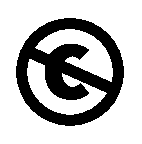
\includegraphics[scale=.25]{eps/Cc-public_domain_mark_white}\ \ 
Это произведение находится в общественном достоянии.

\ 

\noindent\texttt{https://anton-petrunin.github.io/kiselyov-2D/} 

\mainmatter

\subsection*{Предварительные понятия}

\paragraph{}\label{1938/s1}
В стереометрии изучаются геометрические тела и пространственные фигуры, не все точки которых лежат в одной плоскости.
Пространственные фигуры изображаются на плоскости по определенным правилам, основанным на геометрических свойствах, которые производят на глаз приблизительно такое же впечатление, как и сама фигура.

Один из способов изображения пространственных фигур на плоскости будет указан в дальнейшем (§§~\ref{1938/s54}---\ref{1938/s66}).


\chapter{Прямые и плоскости}

\section{Определение положения плоскости}


\begin{figure}[h!]
\centering
\includegraphics{ris/ris-1}
\caption{}
\end{figure} 

\paragraph{Изображение плоскости.}\label{1938/s2}
В обыденной жизни многие предметы, поверхность которых напоминает геометрическую плоскость, имеют форму прямоугольника: переплет книги, оконное стекло, поверхность письменного стола и т.~п.
При этом если смотреть на эти предметы под углом и с большего расстояния, то они представляются нам имеющими форму параллелограмма.
Поэтому принято изображать плоскость на рисунке в виде параллелограмма.%
\footnote{Наряду с указанным изображением плоскости возможно и такое, как на рис.~15---17 и др. (Прим. ред.)%??? не нужно этого
}
Эту плоскость обычно обозначают одной буквой, например «плоскость $M$» (рис.~1).

\paragraph{Основные свойства плоскости.}\label{1938/s3}
Укажем следующие свойства плоскости, которые принимаются без доказательства, т.~е. являются аксиомами:

1) \emph{Если две точки прямой принадлежат плоскости, то и каждая точка этой прямой принадлежит плоскости.}

2) \emph{Если две плоскости имеют общую точку, то они пересекаются по прямой, проходящей через эту точку.}

3) \emph{Через всякие три точки, не лежащие на одной прямой, можно провести плоскость, и притом только одну.}


\paragraph{} \label{1938/s4}
\so{Следствия}. Из последнего предложения можно вывести следствия:

1) \emph{Через прямую и точку вне ее можно провести плоскость (и только одну).} Действительно, точка вне прямой вместе с какими-нибудь двумя точками этой прямой составляют три точки, через которые можно провести плоскость (и притом одну). %???a почему прямая лежит на плоскости

2) \emph{Через две пересекающиеся прямые можно провести плоскость (и только одну).} Действительно, взяв точку пересечения и еще по одной точке на каждой прямой, мы будем иметь три точки, через которые можно провести плоскость (и притом одну). %???a почему прямая лежит на плоскости

3) \emph{Через две параллельные прямые можно провести только одну плоскость.} Действительно, параллельные прямые, по определению, лежат в одной плоскости;
эта плоскость единственная, так как через одну из параллельных и какую-нибудь точку другой можно провести не более одной плоскости.


\paragraph{Вращение плоскости вокруг прямой.}\label{1938/s5} 
\textbf{\emph{Через каждую прямую в пространстве можно провести бесчисленное множество плоскостей.}}

\begin{figure}[h!]
\centering
\includegraphics{ris/ris-2}
\caption{}
\end{figure} 

В самом деле, пусть дана прямая $a$ (рис.~2).
Возьмем какую-нибудь точку $A$ вне ее. 
Через точку $A$ и прямую $a$ проходит единственная плоскость (§~\ref{1938/s4}).
Назовем ее плоскостью $M$.
Возьмем новую точку $B$ вне плоскости $M$.
Через точку $B$ и прямую $a$ в свою очередь проходит плоскость.
Назовем ее плоскостью $N$. 
Она не может совпадать с $M$, так как в ней лежит точка $B$, которая не принадлежит плоскости $M$.
Мы можем далее взять в пространстве еще новую точку $C$ вне плоскостей $M$ и $N$.
Через точку $C$ и прямую $a$ проходит новая плоскость.
Назовем ее $P$.
Она не совпадает ни с $M$, ни с $N$, так как в ней находится точка $C$, не принадлежащая ни плоскости $M$, ни плоскости $N$.
Продолжая брать в пространстве все новые и новые точки, мы будем таким путем получать все новые и новые плоскости, проходящие через данную прямую $a$.
Таких плоскостей будет бесчисленное множество.

Все эти плоскости можно рассматривать как различные положения одной и той же плоскости, которая вращается вокруг прямой $a$.
Мы можем, следовательно, высказать еще одно свойство плоскости: {плоскость может вращаться вокруг всякой прямой, лежащей в этой плоскости.}

\paragraph{Задачи на построение в пространстве.}\label{1938/s6}
Все построения, которые делались в планиметрии, выполнялись в одной плоскости при помощи чертежных инструментов.
Для построений в пространстве чертежные инструменты становятся уже непригодными, так как чертить фигуры в пространстве невозможно.
Кроме того, при построениях в пространстве появляется еще новый элемент --- \textbf{плоскость}, построение которой в пространстве нельзя выполнять столь простыми средствами, как построение прямой на плоскости.

Поэтому при построениях в пространстве необходимо точно {определить, что значит выполнить то или иное построение} и, в частности, что значит построить плоскость в пространстве.
Во всех построениях в пространстве мы будем предполагать, что:

1) плоскость может быть построена, если найдены элементы, определяющие ее положение в пространстве (§§~\ref{1938/s3} и \ref{1938/s4}), т.~е. что мы умеем построить плоскость, проходящую через три данные точки, через прямую и точку вне ее, через две пересекающиеся или две параллельные прямые;

2) если даны две пересекающиеся плоскости, то дана и линия их пересечения, т.~е. мы умеем найти линию пересечения двух плоскостей;

3) если в пространстве дана плоскость, то мы можем выполнять в ней все построения, которые выполнялись в планиметрии.

{Выполнить какое-либо построение в пространстве --- это значит свести его к конечному числу только что указанных основных построений.}
При помощи этих основных задач можно решать и задачи более сложные.

В этих предложениях и решаются задачи на построение в стереометрии.

\paragraph{Пример задачи на построение в пространстве.}\label{1938/s7}\ 

\so{Задача}.
\emph{Найти точку пересечения данной прямой $a$ \emph{(рис.~3)} с данной плоскостью $P$.}

\begin{figure}[h!]
\centering
\includegraphics{ris/ris-3}
\caption{}
\end{figure} 

Возьмем на плоскости $P$ какую-либо точку $A$.
Через точку $A$ и прямую $a$ проводим плоскость $Q$.
Она пересекает плоскость $P$ по некоторой прямой $b$.
В плоскости $Q$ находим точку $C$ пересечения прямых $a$ и $b$.
Эта точка и будет искомой.
Если прямые $a$ и $b$ окажутся параллельными, то задача не будет иметь решения.



\section{Параллельные прямые и плоскости}

\subsection*{Параллельные прямые}

\paragraph{Предварительное замечание.}\label{1938/s8}
Две прямые могут быть расположены в пространстве так, что через них нельзя провести плоскость.
Возьмем, например (рис.~4), две такие прямые $AB$ и $DE$, из которых одна пересекает некоторую плоскость $P$, а другая лежит на ней, но не проходит через точку ($C$) пересечения первой прямой и плоскости $P$.
Через такие две прямые нельзя провести плоскость, потому что в противном случае через прямую $DE$ и точку $C$ проходили бы две различные плоскости:
одна $P$, пересекающая прямую $AB$, и другая, содержащая ее, а это невозможно (§~\ref{1938/s3}).

\begin{figure}[h!]
\centering
\includegraphics{ris/ris-4}
\caption{}
\end{figure}

Две прямые, не лежащие в одной плоскости, конечно, не пересекаются, сколько бы их ни продолжали;
однако их не называют параллельными, оставляя это название для таких прямых, которые, \so{находясь в одной плоскости}, не пересекаются, сколько бы их ни продолжали.

Две прямые, не лежащие в одной плоскости, называются \textbf{скрещивающимися}.

\subsection*{Прямая и плоскость, параллельные между собой}

\paragraph{}\label{1938/s9}
\so{Определение}. Плоскость и прямая, не лежащая в этой плоскости, называются \textbf{параллельными}, если они не пересекаются, сколько бы их ни продолжали.

\paragraph{}\label{1938/s10}
\so{Теорема}. \textbf{\emph{Если прямая}} ($AB$, рис.~5) \textbf{\emph{параллельна какой-нибудь прямой}} ($CD$), \textbf{\emph{расположенной в плоскости}} ($P$), \textbf{\emph{то она параллельна самой плоскости.}}

\begin{figure}[h!]
\centering
\includegraphics{ris/ris-5}
\caption{}
\end{figure}

Проведем через $AB$ и $CD$ плоскость $R$ и предположим, что прямая $AB$ где-нибудь пересекается с плоскостью $P$.
Тогда точка пересечения, находясь на прямой $AB$, должна принадлежать также и плоскости $R$, на которой лежит прямая $AB$, в то же время точка пересечения, конечно, должна принадлежать и плоскости $P$.
Значит, точка пересечения, находясь одновременно и на плоскости $R$, и на плоскости $P$, должна лежать на прямой $CD$, по которой пересекаются эти плоскости;
следовательно, прямая $AB$ пересекается с прямой $CD$.
Но это невозможно, так как по условию $AB\parallel CD$.
Значит, нельзя допустить, чтобы прямая $AB$ пересекалась с плоскостью $P$, и потому $AB\parallel P$.

\paragraph{}\label{1938/s11}
\so{Теорема}. \textbf{\emph{Если плоскость}} ($R$, рис.~5) \textbf{\emph{проходит через прямую}} ($AB$), \textbf{\emph{параллельную другой плоскости}} ($P$), \textbf{\emph{и пересекает эту плоскость, то линия пересечения}} ($CD$) \textbf{\emph{параллельна первой прямой}} ($AB$).

Действительно, во-первых, прямая $CD$ лежит в одной плоскости с прямой $AB$, во-вторых, эта прямая не может пересечься с прямой $AB$, потому что в противном случае прямая $AB$ пересекалась бы с плоскостью $P$, что невозможно.

\paragraph{}\label{1938/s12}
\so{Следствие} 1.
\emph{Если прямая} ($AB$, рис.~6) \emph{параллельна каждой из двух пересекающихся плоскостей} ($P$ и $Q$), \emph{то она параллельна линии их пересечения} ($CD$).

\begin{figure}[h!]
\centering
\includegraphics{ris/ris-6-7}
\caption{}
\end{figure}

Проведем плоскость через $AB$ и какую-нибудь точку $M$ прямой $CD$.
Эта плоскость должна пересечься с плоскостями $P$ и $Q$ по прямым, параллельным $AB$ и проходящим через точку $M$.
Но через точку $M$ можно провести только одну прямую, параллельную $AB$;
значит, две линии пересечения проведенной плоскости с плоскостями $P$ и $Q$ должны слиться в одну прямую.
Эта прямая, находясь одновременно на плоскости $P$ и на плоскости $Q$, должна совпадать с прямой $CD$, по которой плоскости $P$ и $Q$ пересекаются;
значит, $CD \parallel AB$.

\paragraph{}\label{1938/s13}
\so{Следствие} 2.
\emph{Если две прямые} ($AB$ и $CD$, рис.~7) \emph{параллельны третьей прямой} ($EF$), \emph{то они параллельны между собой.}

Проведем плоскость $M$ через параллельные прямые $AB$ и $EF$.
Так как $CD \parallel EF$, то $CD \parallel M$ (§10).

\begin{figure}[h!]
\centering
\includegraphics{ris/ris-8}
\caption{}
\end{figure}

Проведем также плоскость $N$ через $CD$ и некоторую точку $A$ прямой $AB$.
Так как $EF\parallel CD$, то $EF\parallel N$.
Значит, плоскость $N$ должна пересечься с плоскостью $M$ по прямой, параллельной $EF$ (§11) и в то же время проходящей через точку $A$.
Но в плоскости $M$ через $A$ проходит единственная прямая, параллельная $EF$, именно прямая $AB$.
Следовательно, плоскость $N$ пересекается с $M$ по прямой $AB$, значит, $CD \parallel AB$.


\subsection*{Параллельные плоскости}

\paragraph{}\label{1938/s14}
\so{Определение}. Две плоскости называются \textbf{параллельными}, если они не пересекаются, сколько бы их ни продолжали.

\paragraph{}\label{1938/s15}
\so{Теорема}. \textbf{\emph{Если две пересекающиеся прямые}} ($AB$ и $AC$, рис.~8) \textbf{\emph{одной плоскости}} ($P$) \textbf{\emph{соответственно параллельны двум прямым}} ($A_1B_1$ и $A_1C_1$) \textbf{\emph{другой плоскости}} ($Q$), \textbf{\emph{то эти плоскости параллельны}}.

Прямые $AB$ и $AC$ параллельны плоскости $Q$ (§~\ref{1938/s10}).

Допустим, что плоскости $P$ и $Q$ пересекаются по некоторой прямой $DE$ (рис.~8).
В таком случае $AB \parallel DE$ и $AC \parallel DE$ (§~\ref{1938/s11}).

Таким образом, в плоскости $P$ через точку $A$ проходят две прямые $AB$ и $AC$, параллельные прямой $DE$, что невозможно.
Значит, плоскости $P$ и $Q$ не пересекаются.

\paragraph{}\label{1938/s16}
\so{Теорема}. \textbf{\emph{Если две параллельные плоскости}} ($P$ и $Q$, рис.~9) \textbf{\emph{пересекаются третьей плоскостью}} ($R$), \textbf{\emph{то линии пересечения}} ($AB$ и $CD$) \textbf{\emph{параллельны.}}

Действительно, во-первых, прямые $AB$ и $CD$ находятся в одной плоскости ($R$);
во-вторых, они не могут пересечься, так как в противном случае пересекались бы плоскости $P$ и $Q$, что противоречит условию.

\paragraph{}\label{1938/s17}
\so{Теорема}. \textbf{\emph{Отрезки параллельных прямых}} ($AC$ и $BD$, рис.~9), \textbf{\emph{заключенные между параллельными плоскостями}} ($P$ и $Q$), \textbf{\emph{равны.}}

Через параллельные прямые $AC$ и $BD$ проведем плоскость $R$;
она пересечет плоскости $P$ и $Q$ по параллельным прямым $AB$ и $CD$;
следовательно, фигура $ABDC$ есть параллелограмм, и потому $AC = BD$.

\paragraph{}\label{1938/s18}
\so{Теорема}. \textbf{\emph{Два угла}} ($BAC$ и $B_1A_1C_1$, рис.~10) \textbf{\emph{с соответственно параллельными и одинаково направленными сторонами равны и лежат в параллельных плоскостях}} ($P$ и $Q$).

\begin{figure}[h!]
\centering
\includegraphics{ris/ris-9-10}
\caption{}
\end{figure}

Что плоскости $P$ и $Q$ параллельны, было доказано выше (§~\ref{1938/s15});
остается доказать, что углы $A$ и $A_1$ равны.

Отложим на сторонах углов произвольные, но равные отрезки $AB\z=A_1B_1$, $AC=A_1C_1$ и проведем прямые $AA_1$, $BB_1$, $CC_1$, $BC$ и $B_1C_1$.
Так как отрезки $AB$ и $A_1B_1$ равны и параллельны, то фигура $ABB_1A_1$ есть параллелограмм;
поэтому отрезки $AA_1$ и $BB_1$ равны и параллельны.
По той же причине равны и параллельны отрезки $AA_1$ и $CC_1$, следовательно, $BB_1\parallel CC_1$ и $BB_1=CC_1$.
Поэтому $BC=B_1C_1$ и $\triangle ABC=\triangle A_1B_1C_1$ (по трем сторонам);
значит, $\angle A=\angle A_1$.

\subsection*{Задачи на построение}

\paragraph{}\label{1938/s19}
\emph{Через точку} ($A$, рис.~11), \emph{расположенную вне данной прямой} ($a$), \emph{в пространстве провести прямую, параллельную данной прямой} ($a$).

\so{Решение}.
Через прямую $a$ и точку $A$ проводим плоскость $M$.
В этой плоскости строим прямую $b$, параллельную прямой $a$.

Задача имеет единственное решение.
В самом деле, искомая прямая должна лежать с прямой $a$ в одной плоскости.
В этой же плоскости должна находиться точка $A$, через которую проходит искомая прямая.
Значит, эта плоскость должна совпадать с $M$.
Но в плоскости $M$ через точку $A$ можно провести только одну прямую, параллельную прямой~$a$.

\begin{figure}[h!]
\centering
\includegraphics{ris/ris-11-12}
\caption{}
\end{figure}

\paragraph{}\label{1938/s20}
\emph{Через данную точку} ($A$, рис.~12) \emph{провести плоскость, параллельную данной плоскости} ($P$), \emph{не проходящей через точку} $A$.

\so{Решение}.
Проводим на плоскости $P$ через какую-либо точку $B$ две какие-либо прямые $BC$ и $BD$.
Построим две вспомогательные плоскости: плоскость $M$ --- через точку $A$ и прямую $BC$ и плоскость $N$ --- через точку $A$ и прямую $BD$.
Искомая плоскость, параллельная плоскости $P$, должна пересечь плоскость $M$ по прямой, параллельной $BC$, а плоскость $N$ --- по прямой, параллельной $BD$ (§~\ref{1938/s16}).
Отсюда вытекает такое построение: через точку $A$ проводим в плоскости $M$ прямую $AC_1\parallel BC$, а в плоскости $N$ прямую $AD_1\parallel BD$.

Через прямые $AC_1$ и $AD_1$ проводим плоскость $Q$.
Она и будет искомой.
В самом деле, стороны угла $D_1AC_1$, расположенного в плоскости $Q$, параллельны сторонам угла $DBC$, расположенного в плоскости $P$.
Следовательно, $Q\parallel P$.

Так как в плоскости $M$ через точку $A$ можно провести лишь одну прямую, параллельную $BC$, а в плоскости $N$ через точку $A$ лишь одну прямую, параллельную $BD$, то задача имеет единственное решение.
Следовательно, через каждую точку пространства можно провести единственную плоскость, параллельную данной плоскости.

\paragraph{}\label{1938/s21}
\emph{Через данную прямую} ($a$, рис.~13) \emph{провести плоскость, параллельную другой данной прямой} ($b$).

\begin{figure}[h!]
\centering
\includegraphics[scale=.7]{ris/ris-13-14}
\caption{}
\end{figure}

\so{Решение}.
1-й \so{случай}.
Прямые $a$ и $b$ не параллельны.
Через какую-нибудь точку $A$ прямой $a$ проводим прямую $b_1$, параллельную $b$;
через прямые $a$ и $b_1$ проводим плоскость.
Она и будет искомой (§~\ref{1938/s10}).
Задача имеет в этом случае единственное решение.

2-й \so{случай}.
Прямые $a$ и $b$ параллельны.
В этом случае задача неопределенна: всякая плоскость, проходящая через прямую $a$, будет параллельна прямой $b$.

\paragraph{Пример более сложной задачи на построение.}\label{1938/s22}
Даны две скрещивающиеся прямые ($a$ и $b$, рис.~14) и точка $A$, не лежащая ни на одной из данных прямых.
Провести через точку $A$ прямую, пересекающую обе данные прямые ($a$ и $b$).

\so{Решение}.
Так как искомая прямая должна проходить через точку $A$ и пересекать прямую $a$, то она должна лежать в плоскости, проходящей через прямую $a$ и точку $A$ (так как две ее точки должны лежать в этой плоскости: точка $A$ и точка пересечения с прямой $a$).
Совершенно так же убеждаемся, что искомая прямая должна лежать в плоскости, проходящей через точку $A$ и прямую $b$.
Следовательно, она должна служить линией пересечения этих двух плоскостей.
Отсюда такое построение.
Через точку $A$ и прямую $a$ проводим плоскость $M$;
через точку $A$ и прямую $b$ проводим плоскость $N$.
Берем прямую $c$ пересечения плоскостей $M$ и $N$.
Если прямая $c$ не параллельна ни одной из данных прямых, то она пересечется с каждой из данных прямых (так как с каждой из них она лежит в одной плоскости: $a$ и $c$ лежат в плоскости $M$, $b$ и $c$ --- в плоскости $N$).
Прямая $c$ будет в этом случае искомой.
Если же $a\parallel c$ или $b\parallel c$, то задача не имеет решения.

\section{Перпендикуляр и наклонные к плоскости}

Поставим задачу определить, в каком случае прямая может считаться перпендикулярной к плоскости.
Докажем предварительно следующее предложение:

\paragraph{}\label{1938/s23}
\so{Теорема}.
\textbf{\emph{Если прямая}} ($AA_1$, рис.~15), \textbf{\emph{пересекающаяся с плоскостью}} ($MN$), \textbf{\emph{перпендикулярна к каким-нибудь двум прямым}} ($OB$ и $OC$), \textbf{\emph{проведенным на этой плоскости через точку пересечения}} ($O$) \textbf{\emph{данной прямой и плоскости, то она перпендикулярна и ко всякой третьей прямой}} ($OD$), \textbf{\emph{проведенной на плоскости через ту же точку пересечения}} ($O$).

\begin{figure}[h!]
\centering
\includegraphics[scale=.7]{ris/ris-15}
\caption{}
\end{figure}

Отложим на прямой $AA_1$ произвольной длины, но равные отрезки $OA$ и $OA_1$ и проведем на плоскости какую-нибудь прямую, которая пересекала бы три прямые, исходящие из точки $O$, в каких-нибудь точках $C$, $D$ и $B$.
Эти точки соединим с точками $A$ и $A_1$.
Мы получим тогда несколько треугольников.
Рассмотрим их в такой последовательности.

Сначала возьмем треугольники $ACB$ и $A_1CB$;
они равны, так как у них $CB$ --- общая сторона, $AC=A_1C$ как наклонные к прямой $AA_1$, одинаково удаленные от основания $O$ перпендикуляра $OC$;
по той же причине $AB=A_1B$.
Из равенства этих треугольников следует, что $\angle ABC=\angle A_1BC$.

После этого перейдем к треугольникам $ADB$ и $A_1DB$;
они равны, так как у них $DB$ --- общая сторона, $AB=A_1B$ и $\angle ABD=\angle A_1BD$.
Из равенства этих треугольников выводим, что $AD=A_1D$.

Теперь возьмем треугольники $AOD$ и $A_1OD$;
они равны, так как имеют соответственно равные стороны.
Из их равенства выводим, что $\angle AOD=\angle A_1OD$;
а так как эти углы смежные, то, следовательно, $AA_1\perp OD$.

\paragraph{}\label{1938/s24}
\so{Определение}.
Прямая называется \textbf{перпендикулярной к плоскости}, если она, пересекаясь с этой плоскостью, образует прямой угол с каждой прямой, проведенной на плоскости через точку пересечения.
В этом случае говорят также, что плоскость перпендикулярна к прямой.

Из предыдущей теоремы (§~\ref{1938/s23}) следует, что прямая перпендикулярна к плоскости, если она перпендикулярна к двум прямым, лежащим в данной плоскости и проходящим через точку пересечения данной прямой и плоскости.

Прямая, пересекающая плоскость, но не перпендикулярная к ней, называется \textbf{наклонной} к этой плоскости.
Точка пересечения прямой с плоскостью называется \textbf{основанием}, перпендикуляра или наклонной.


\paragraph{Сравнительная длина перпендикуляра и наклонных.}\label{1938/s25}%
\footnote{Для краткости термины «перпендикуляр» и «наклонная» употребляются вместо «отрезок перпендикуляра, ограниченный данной точкой и основанием перпендикуляра», и «отрезок наклонной, ограниченный данной точкой и основанием наклонной».}
Когда из одной точки $A$ (рис.~16) проведены к плоскости перпендикуляр $AB$ и наклонная $AC$, условимся называть \textbf{проекцией} наклонной на плоскость $P$ отрезок $BC$, соединяющий основание перпендикуляра и основание наклонной.
Таким образом, отрезок $BC$ есть проекция наклонной $AC$, отрезок $BD$ есть проекция наклонной $AD$ и т.~д.

\paragraph{}\label{1938/s26}
\so{Теорема}.
\textbf{\emph{Если из одной и той же точки}} ($A$, рис.~16), \textbf{\emph{взятой вне плоскости}} ($P$), \textbf{\emph{проведены к этой плоскости перпендикуляр}} ($AB$) \textbf{\emph{и какие-нибудь наклонные}} ($AC$, $AD$, $AE$,\dots), \textbf{\emph{то:}}

1) \textbf{\emph{две наклонные, имеющие равные проекции, равны;}}

2) \textbf{\emph{из двух наклонных та больше, проекция которой больше.}} 

\begin{figure}[h!]
\centering
\includegraphics[scale=.7]{ris/ris-16}
\caption{}
\end{figure}

Вращая прямоугольные треугольники $ABC$ и $ABD$ вокруг катета $AB$, мы можем совместить их плоскости с плоскостью $\triangle ABE$.
Тогда все наклонные будут лежать в одной плоскости с перпендикуляром, а все проекции расположатся на одной прямой.
Таким образом, доказываемые теоремы приводятся к аналогичным теоремам планиметрии.

\so{Замечание}.
Так как $AB$ есть катет прямоугольного треугольника, а каждая из наклонных $AC, AD, AE,\dots$ есть гипотенуза, то перпендикуляр $AB$ меньше всякой наклонной;
значит, перпендикуляр, опущенный из точки на плоскость, есть наименьший из всех отрезков, соединяющих данную точку с любой точкой плоскости, и потому он принимается за меру расстояния точки $A$ от плоскости $P$.

\paragraph{}\label{1938/s27}
\so{Обратные теоремы}.
\textbf{\emph{Если из одной и той же точки, взятой вне плоскости, проведены перпендикуляр и какие-нибудь наклонные, то: 1) равные наклонные имеют равные проекции;
2) из двух проекций та больше, которая соответствует большей наклонной.}}

Доказательство (от противного) предоставляем самим учащимся.

\paragraph{Теорема о трех перпендикулярах.}\label{1938/s28}
Приведем еще следующую теорему о перпендикулярах, которая понадобится нам впоследствии.

 \so{Теорема}.
\textbf{\emph{Прямая}} ($DE$, рис.~17), \textbf{\emph{проведенная на плоскости}} ($P$) \textbf{\emph{через основание наклонной}} ($AC$) \textbf{\emph{перпендикулярно к ее проекции}} ($BC$), \textbf{\emph{перпендикулярна и к самой наклонной.}}

Отложим произвольные, но равные отрезки $CD$ и $CE$ и соединим прямолинейными отрезками точки $A$ и $B$ с точками $D$ и $E$.
Тогда будем иметь: $BD=BE$ как наклонные к прямой $DE$, одинаково удаленные от основания $C$ перпендикуляра $BC$;
$AD=AE$ как наклонные к плоскости $P$, имеющие равные проекции $BD$ и $BE$.
Вследствие этого $\triangle ADE$ равнобедренный, и потому его медиана $AC$ перпендикулярна к основанию $DE$.

Эта теорема носит название теоремы о трех перпендикулярах.
Действительно, в ней говорится о связи, соединяющей следующие три перпендикуляра: 1) $AB$ к плоскости $P$, 2) $BC$ к прямой $DE$ и 3) $AC$ к той же прямой $DE$.

\begin{figure}[h!]
\centering
\includegraphics[scale=.7]{ris/ris-17}
\caption{}
\end{figure}

\paragraph{}\label{1938/s29}
\so{Обратная теорема}.
\textbf{\emph{Прямая}} ($DE$, рис.~17), \textbf{\emph{проведенная на плоскости}} ($P$) \textbf{\emph{через основание наклонной}} ($AC$) \textbf{\emph{перпендикулярно к этой наклонной, перпендикулярна и к ее проекции.}}

Сделаем те же построения, что и при доказательстве прямой теоремы.
Отложим произвольные, но равные отрезки $CD$ и $CE$ и соединим прямолинейными отрезками точки $A$ и $B$ с точками $D$ и $E$, тогда будем иметь: $AD=AE$ как наклонные к прямой $DE$, одинаково удаленные от основания $C$ перпендикуляра $AC$;
$BD=BE$ как проекции равных наклонных $AD$ и $AE$.
Вследствие этого $\triangle BDE$ равнобедренный, и потому его медиана $BC$ перпендикулярна к основанию $DE$.



\section[Параллельность и перпендикулярность]{Параллельность и перпендикулярность\\ прямых и плоскостей}


\paragraph{Предварительное замечание.}\label{1938/s30}
Параллельность прямых и плоскостей в пространстве и перпендикулярность прямой к плоскости находятся в некоторой зависимости.
Именно наличие параллельности одних элементов влечет перпендикулярность других, и, обратно, из перпендикулярности одних элементов можно сделать заключение о параллельности других.
Эта связь между параллельностью и перпендикулярностью прямых и плоскостей в пространстве выражается следующими теоремами.

\paragraph{}\label{1938/s31}
\so{Теорема}.
\textbf{\emph{Если плоскость}} ($P$, рис.~18) \textbf{\emph{перпендикулярна к одной из параллельных прямых}} ($AB$), \textbf{\emph{то она перпендикулярна и к другой}} ($CD$).

Проведем через точку $B$ на плоскости $P$ две какие-нибудь прямые $BE$ и $BF$, а через точку $D$ проведем прямые $DG$ и $DH$, соответственно параллельные прямым $BE$ и $BF$.
Тогда будем иметь: $\angle ABE=\angle CDG$ и $\angle ABF = \angle CDH$ как углы с параллельными сторонами.
Но углы $ABE$ и $ABF$ прямые, так как $AB\perp P$, значит, углы $CDG$ и $CDH$ также прямые (§~\ref{1938/s18}).
Следовательно, $CD \perp P$ (§~\ref{1938/s24}).

\begin{figure}[h!]
\centering
\includegraphics[scale=.7]{ris/ris-18-19}
\caption{}
\end{figure}

\paragraph{}\label{1938/s32}
\so{Обратная теорема}.
\textbf{\emph{Если две прямые}} ($AB$ и $CD$, рис.~19) \textbf{\emph{перпендикулярны к одной и той же плоскости}} ($P$), \textbf{\emph{то они параллельны.}}

Предположим противное, т.~е. что прямые $AB$ и $CD$ не параллельны.
Проведем тогда через точку $D$ прямую, параллельную $AB$. %надо сказать, что D на P???
При нашем предположении это будет какая-нибудь прямая $DC_1$, не сливающаяся с $DC$.
Согласно прямой теореме прямая $DC$ будет перпендикулярна к плоскости $P$.
Проведем через $CD$ и $C_1D$ плоскость $Q$ и возьмем линию ее пересечения $DE$ с плоскостью $P$.
Так как (на основании предыдущей теоремы) $C_1D \perp P$, то $\angle C_1DE$ прямой, а так как по условию $CD \perp P$, то $\angle CDE$ также прямой.
Таким образом, окажется, что в плоскости $Q$ к прямой $DE$ из одной ее точки $D$ восставлены два перпендикуляра $DC$ и $DC_1$.
Так как это невозможно, то нельзя допустить, чтобы прямые $AB$ и $CD$ были не параллельны.

\paragraph{}\label{1938/s33}
\so{Теорема}.
\textbf{\emph{Если прямая}} ($BB_1$, рис.~20) \textbf{\emph{перпендикулярна к одной из параллельных плоскостей}} ($P$), \textbf{\emph{то она перпендикулярна и к другой}} ($Q$).

Проведем через прямую $BB_1$ какие-нибудь две плоскости $M$ и $N$, каждая из которых пересекается с $P$ и $Q$ по параллельным прямым: одна --- по параллельным прямым $BC$ и $B_1C_1$, другая --- по параллельным прямым $BD$ и $B_1D_1$.
Согласно условию прямая $BB_1$ перпендикулярна к прямым $BC$ и $BD$;
следовательно, она также перпендикулярна к параллельным им прямым $B_1C_1$ и $B_1D_1$, а потому перпендикулярна и к плоскости $Q$, на которой лежат прямые $B_1C_1$ и $B_1D_1$.

\begin{figure}[h!]
\centering
\includegraphics[scale=.7]{ris/ris-20-21}
\caption{}
\end{figure}

\paragraph{}\label{1938/s34}
\so{Обратная теорема}.
\textbf{\emph{Если две плоскости}} ($P$ и $Q$, рис.~21) \textbf{\emph{перпендикулярны к одной и той же прямой}} ($AB$), \textbf{\emph{то они параллельны.}}

Предположим противное, т.~е. что плоскости $P$ и $Q$ пересекаются.
Возьмем на линии их пересечения какую-нибудь точку $C$ и проведем плоскость $R$ через $C$ и прямую $AB$.
Плоскость $R$ пересечет плоскости $P$ и $Q$ соответственно по прямым $AC$ и $BC$.
Так как $AB\perp P$, то $AB\perp AC$, и так как $AB\perp Q$, то $AB\perp BC$.
Таким образом, в плоскости $R$ мы будем иметь два перпендикуляра к прямой $AB$, проходящих через одну и ту же точку $C$, перпендикуляры $AC$ и $BC$.
Так как это невозможно, то предположение, что плоскости $P$ и $Q$ пересекаются, неверно.
Значит, они параллельны.

\subsection*{Задачи на построение}

\paragraph{}\label{1938/s35}
\emph{Через данную точку в пространстве провести плоскость, перпендикулярную к данной прямой} ($AB$).

\so{Решение}.
1-й \so{случай}.
Данная точка $C$ лежит на прямой $AB$ (рис.~22).

Проведем через прямую $AB$ какие-нибудь две плоскости $P$ и $Q$.
Искомая плоскость должна пересекать эти плоскости по прямым, перпендикулярным к прямой $AB$ (§24).

Отсюда построение: через $AB$ проводим две произвольные плоскости $P$ и $Q$.
В каждой из этих плоскостей восставляем перпендикуляр к прямой $AB$ в точке $C$ (в плоскости $P$ --- перпендикуляр $CD$, в плоскости $Q$ --- перпендикуляр $CE$.
Плоскость, проходящая через прямые $CD$ и $CE$, есть искомая.

\begin{figure}[h!]
\centering
\includegraphics[scale=.7]{ris/ris-22}
\caption{}
\end{figure}

2-й \so{случай}.
Данная точка $D$ не лежит на прямой $AB$ (рис.~22).
Через точку $D$ и прямую $AB$ проводим плоскость $P$ и в этой плоскости строим прямую $DC$, перпендикулярную к $AB$.
Через прямую $AB$ проводим произвольно вторую плоскость $Q$ и в этой плоскости строим прямую $CE$, перпендикулярную к $AB$.
Искомая плоскость должна пересечь плоскости $P$ и $Q$ по прямым, перпендикулярным к $AB$.

Отсюда построение: через точку $D$ проводим в плоскости $P$ прямую $DC$, перпендикулярную к $AB$.
Прямая $DC$ пересечет прямую $AB$ в некоторой точке $C$.
Через точку $C$ проводим в плоскости $Q$ прямую $CE$ перпендикулярно к $AB$.
Плоскость, проходящая через прямые $CD$ и $CE$, --- искомая.

Так как в каждой из плоскостей $P$ и $Q$ через данную точку можно провести лишь одну прямую, перпендикулярную к данной, то задача в обоих случаях имеет одно решение, т.~е. через каждую точку в пространстве можно провести лишь одну плоскость, перпендикулярную к данной прямой.

\paragraph{}\label{1938/s36}
\emph{Через данную точку} ($O$) \emph{пространства провести прямую, перпендикулярную к данной плоскости} ($P$).

1-й \so{случай}.
Точка $O$ лежит на плоскости $P$ (рис.~23).
Проведем на плоскости $P$ через точку $O$ две какие-либо взаимно перпендикулярные прямые $OA$ и $OB$.
Проведем, далее, через прямую $OA$ какую-либо новую плоскость $Q$ и на этой плоскости $Q$ построим прямую $OC$, перпендикулярную к $OA$.
Через прямые $OB$ и $OC$ проведем новую плоскость $R$ и построим в ней прямую $OM$, перпендикулярную к $OB$.
Прямая $OM$ и будет искомым перпендикуляром к плоскости $P$.

Действительно, так как $OA \perp OB$ и $OA \perp OC$, то прямая $AO$ перпендикулярна к плоскости $R$ и, следовательно, $OA \perp OM$.
Таким образом, мы видим, что $OM\perp OA$ и $OM\perp OB$;
следовательно, $OM$ перпендикулярна к плоскости $P$.

\begin{figure}[h!]
\centering
\includegraphics[scale=.7]{ris/ris-23-24}
\caption{}
\end{figure}

2-й \so{случай}.
Точка $O$ не лежит на плоскости $P$ (рис.~24).
Возьмем на плоскости $P$ какую-нибудь точку $A$ и выполним для нее предыдущее построение.
Мы получим тогда прямую $AB$, перпендикулярную к плоскости $P$.
После этого через точку $O$ проводим прямую, параллельную $AB$.
Эта прямая и будет искомой (§31).

Задача в обоих случаях имеет одно решение.
В самом деле, так как два перпендикуляра к одной и той же плоскости параллельны, то через одну и ту же точку $O$ нельзя провести двух перпендикуляров к плоскости $P$.
Следовательно, через каждую точку в пространстве можно провести одну и только одну прямую, перпендикулярную к данной плоскости.

\paragraph{Пример более сложной задачи.}\label{1938/s37}
\emph{Даны две скрещивающиеся прямые} ($a$ и $b$, рис.~25).
\emph{Построить прямую, пересекающую обе данные прямые и перпендикулярную к ним обеим.}

\begin{figure}[h!]
\centering
\includegraphics[scale=.7]{ris/ris-25}
\caption{}
\end{figure}

\so{Решение}.
Проведем через прямую $a$ плоскость $M$, параллельную прямой $b$ (§21).
Из двух каких-нибудь точек прямой $b$ опустим перпендикуляры $AA_1$ и $BB_1$ на плоскость $M$.
Соединим точки $A_1$ и $B_1$ отрезком прямой и найдем точку $C_1$ пересечения прямых $A_1B_1$ и $a$.
Через точку $C_1$ проведем прямую, перпендикулярную к плоскости $M$.

Предоставляем самим учащимся доказать, что эта прямая 1) пересечется с прямой $b$ в некоторой точке $C$ и 2) будет перпендикулярна как к прямой $a$, так и к прямой $b$.
Прямая $CC_1$ будет, следовательно, искомой прямой.

Заметим, что отрезок $CC_1$ меньше всех других отрезков, которые можно получить, соединяя точки прямой $a$ с точками прямой $b$.
В самом деле, возьмем на прямой а какую-нибудь точку $E$ и на прямой $b$ какую-нибудь точку $F$, соединим эти точки отрезком прямой и докажем, что $EF>CC_1$.
Опустим из точки $F$ перпендикуляр $FF_1$ на плоскость $M$.
Тогда будем иметь: $EF>FF_1$ (§26).
Но $FF_1=CC_1$, следовательно $EF>CC_1$.
На этом основании длина отрезка $CC_1$ называется кратчайшим расстоянием между данными прямыми $a$ и $b$.

\section[Углы]{Двугранные углы,
угол прямой с плоскостью,
угол двух скрещивающихся прямых,
многогранные углы}

\subsection*{Двугранные углы}

\paragraph{}\label{1938/s38}
\so{Определения}.
Часть плоскости, лежащая по одну сторону от какой-либо прямой, лежащей в этой плоскости, называется полуплоскостью.
Фигура, образованная двумя полуплоскостями ($P$ и $Q$, рис.~26), исходящими из одной прямой ($AB$), называется \textbf{двугранным углом}.
Прямая $AB$ называется \textbf{ребром}, а полуплоскости $P$ и $Q$ --- сторонами или \textbf{гранями} двугранного угла.

\begin{figure}[h!]
\centering
\includegraphics[scale=.7]{ris/ris-26-28}
\caption{}
\end{figure}

Такой угол обозначается обыкновенно двумя буквами, поставленными у его ребра (двугранный угол $AB$).
Но если при одном ребре лежат несколько двугранных углов, то каждый на них обозначают четырьмя буквами, из которых две средние стоят при ребре, а две крайние --- у граней (например, двугранный угол $SCDR$, рис.~27).

Если из произвольной точки $D$ ребра $AB$ (рис.~28) проведем на каждой грани по перпендикуляру к ребру, то образованный ими угол $CDE$ называется \textbf{линейным углом} двугранного угла.

Величина линейного угла не зависит от положения его вершины на ребре.
Так, линейные углы $CDE$ и $C_1D_1E_1$ равны, потому что их стороны соответственно параллельны и одинаково направлены.

Плоскость линейного угла перпендикулярна к ребру, так как она содержит две прямые, перпендикулярные к нему.
Поэтому для получения линейного угла достаточно грани данного двугранного угла пересечь плоскостью, перпендикулярной к ребру, и рассмотреть получившийся в этой плоскости угол.

\paragraph{Равенство и неравенство двугранных углов.}\label{1938/s39}
Два двугранных угла считаются \textbf{равными}, если они при вложении могут совместиться;
в противном случае тот из двугранных углов считается меньшим, который составит часть другого угла.

Подобно углам в планиметрии двугранные углы могут быть \textbf{смежные}, \textbf{вертикальные} и прочие.

Если два смежных двугранных угла равны между собой, то каждый из них называется прямым двугранным углом.

\so{Теоремы}.
1) \textbf{\emph{Равным двугранным, углам, соответствуют равные линейные углы.}}

2) \textbf{\emph{Большему двугранному углу соответствует больший линейный угол.}}

Пусть $PABQ$ и $P_1A_1B_1Q_1$ (рис.~29) --- два двугранных угла.
Вложим угол $A_1B_1$ в угол $AB$ так, чтобы ребро $A_1B_1$ совпало с ребром $AB$ и грань $P_1$ с гранью $P$.
Тогда если эти двугранные углы равны, то грань $Q_1$ совпадет с гранью $Q$;
если же угол $A_1B_1$ меньше угла $AB$, то грань $Q_1$ займет некоторое положение внутри двугранного угла, например~$Q_2$.

\begin{figure}[h!]
\centering
\includegraphics[scale=.7]{ris/ris-29-30}
\caption{}
\end{figure}

Заметив это, возьмем на общем ребре какую-нибудь точку $B$ и проведем через нее плоскость $R$, перпендикулярную к ребру.
От пересечения этой плоскости с гранями двугранных углов получатся линейные углы.
Ясно, что если двугранные углы совпадут, то у них окажется один и тот же линейный угол $CBD$;
если же двугранные углы не совпадут, если, например, грань $Q_1$ займет положение $Q_2$, то у большего двугранного угла окажется больший линейный угол (именно: $\angle CBD > \angle C_2BD$).

\paragraph{}\label{1938/s40}
\so{Обратные теоремы}.
1) \textbf{\emph{Равным, линейным, углам, соответствуют равные двугранные углы.}}

2) \textbf{\emph{Большему линейному углу соответствует больший двугранный угол.}}

Эти теоремы легко доказываются от противного.

\paragraph{}\label{1938/s41}
\so{Следствия}. 1) \emph{Прямому двугранному углу соответствует прямой линейный угол, и обратно.}

Пусть (рис.~30) двугранный угол $PABQ$ прямой.
Это значит, что он равен смежному углу $QABP_1$.
Но в таком случае линейные углы $CDE$ и $CDE_1$ также равны;
а так как они смежные, то каждый из них должен быть прямой.

Обратно, если равны смежные линейные углы $CDE$ и $CDE_1$, то равны и смежные двугранные углы, т.~е. каждый из них должен быть прямой.

2) \emph{Все прямые двугранные углы равны, потому что у них равны линейные углы.}

Подобным же образом легко доказать, что:

3) \emph{Вертикальные двугранные углы равны.}

4) \emph{Двугранные углы с соответственно параллельными и одинаково} (или противоположно) \emph{направленными гранями равны.}

5) Если за единицу двугранных углов возьмем такой двугранный угол, который соответствует единице линейных углов, то можно сказать, что \emph{двугранный угол измеряется его линейным углом}.

\subsection*{Перпендикулярные плоскости}

\paragraph{}\label{1938/s42}
\so{Определение}.
Две плоскости называются \textbf{взаимно перпендикулярными}, если, пересекаясь, они образуют прямые двугранные углы.

\paragraph{}\label{1938/s43} \so{Теорема} (выражающая признак перпендикулярности двух плоскостей).
\textbf{\emph{Если плоскость}} ($P$, рис.~31) \textbf{\emph{проходит через перпендикуляр}} ($AB$) \textbf{\emph{к другой плоскости}} ($Q$), \textbf{\emph{то она перпендикулярна к этой плоскости.}}

\begin{figure}[h!]
\centering
\includegraphics[scale=.7]{ris/ris-31}
\caption{}
\end{figure}

Пусть $DE$ будет линия пересечения плоскостей $P$ и $Q$.
На плоскости $Q$ проведем $BC \perp DE$.
Тогда угол $ABC$ будет линейным углом двугранного угла $PDEQ$.
Так как прямая $AB$ по условию перпендикулярна к $Q$, то $AB\perp BC$;
значит, угол $ABC$ прямой, а потому и двугранный угол прямой, т.~е. плоскость $P$ перпендикулярна к плоскости~$Q$.

\paragraph{}\label{1938/s44}
\so{Теорема}.
\textbf{\emph{Если две плоскости}} ($P$ и $Q$, рис.~31) \textbf{\emph{взаимно перпендикулярны и к одной из них}} ($Q$) \textbf{\emph{проведен перпендикуляр}} ($AB$), \textbf{\emph{имеющий общую точку}} ($A$) \textbf{\emph{с другой плоскостью}} ($P$), \textbf{\emph{то этот перпендикуляр весь лежит в этой плоскости}}~($P$).

\begin{figure}[h!]
\centering
\includegraphics[scale=.7]{ris/ris-32}
\caption{}
\end{figure}

Предположим, что перпендикуляр $AB$ не лежит в плоскости $P$ (как изображено на рис.~32).
Пусть $DE$ будет линия пересечения плоскостей $P$ и $Q$.
На плоскости $P$ проведем прямую $AC \perp DE$, а на плоскости $Q$ проведем прямую $CF \perp DE$.
Тогда угол $ACF$, как линейный угол прямого двугранного угла, будет прямой.
Поэтому линия $AC$, образуя прямые углы с $DE$ и $CF$, будет перпендикуляром к плоскости $Q$.
Мы будем иметь тогда два перпендикуляра, опущенные из одной и той же точки $A$ на плоскость $Q$, именно $AB$ и $AC$.
Так как это невозможно (§36), то допущение неверно;
значит, перпендикуляр $AB$ лежит в плоскости $P$.

\paragraph{}\label{1938/s45}
\so{Следствие}.
\emph{Линия пересечения} ($AB$ рис.~33) \emph{двух плоскостей} ($P$ и $Q$), \emph{перпендикулярных к третьей плоскости} ($R$), \emph{есть перпендикуляр к этой плоскости}.

\begin{figure}[h!]
\centering
\includegraphics[scale=.7]{ris/ris-33-34}
\caption{}
\end{figure}

Действительно, если через какую-нибудь точку $A$ линии пересечения плоскостей $P$ и $Q$ проведем перпендикуляр к плоскости $R$, то этот перпендикуляр согласно предыдущей теореме должен лежать и в плоскости $Q$, и в плоскости $P$, значит, он сольется с $AB$.

\subsection*{Угол двух скрещивающихся прямых}

\paragraph{}\label{1938/s46}
\so{Определение}.
Углом двух скрещивающихся прямых ($AB$ и $CD$, рис.~34), для которых дано положение и направление, называется угол ($MON$), который получится, если из произвольной точки пространства ($O$) проведем полупрямые ($OM$ и $ON$), соответственно параллельные данным прямым ($AB$ и $CD$) и одинаково с ними направленные.

Величина этого угла не зависит от положения точки $O$, так как если построим указанным путем угол $M_1O_1N_1$ с вершиной в какой-нибудь другой точке $O_1$, то $\angle MON = \angle M_1O_1N_1$, потому что эти углы имеют соответственно параллельные и одинаково направленные стороны.

\subsection*{Угол, образуемый прямой с плоскостью}

\paragraph{Проекция точки и прямой на плоскость.}\label{1938/s47}
Мы говорили ранее (§25), что когда из одной точки проведены к плоскости перпендикуляр и наклонная, то проекцией этой наклонной на плоскость называется отрезок, соединяющий основание перпендикуляра с основанием наклонной.
Дадим теперь более общее определение проекции.

1) \textbf{Ортогональной} (или \textbf{прямоугольной}) \textbf{проекцией} какой-нибудь \textbf{точки} на данную плоскость (например, точки $M$ на плоскость $P$, рис.~35) называется основание ($m$) перпендикуляра, опущенного на эту плоскость из взятой точки.

2) \textbf{Ортогональной проекцией} какой-нибудь \textbf{линии} на плоскость называется геометрическое место проекций всех точек этой линии.

В частности, если проектируемая линия есть прямая (например, $AB$, рис.~35), не перпендикулярная к плоскости ($P$), то проекция ее на эту плоскость есть также прямая.
В самом деле, если мы через прямую $AB$ и перпендикуляр $Mm$, опущенный на плоскость проекций из какой-нибудь одной точки $M$ этой прямой, проведем плоскость $Q$, то эта плоскость должна быть перпендикулярна к плоскости $P$;
поэтому перпендикуляр, опущенный на плоскость $P$ из любой точки прямой $AB$ (например, из точки $N$), должен лежать в этой плоскости $Q$ (§~\ref{1938/s44}) и, следовательно, проекции всех точек прямой $AB$ должны лежать на прямой $ab$, по которой пересекаются плоскости $P$ и $Q$.

Обратно, всякая точка этой прямой $ab$ есть проекция какой-нибудь точки прямой $AB$, так как перпендикуляр, восставленный из любой точки прямой $ab$, лежит на плоскости $Q$ и, следовательно, пересекается с $AB$ в некоторой точке.
Таким образом, прямая $ab$ представляет собой геометрическое место проекций всех точек данной прямой $AB$ и, следовательно, есть ее проекция.

Для краткости вместо «ортогональная проекция» мы будем говорить просто «проекция».

\begin{figure}[h!]
\centering
\includegraphics[scale=.7]{ris/ris-35-36}
\caption{}
\end{figure}

\paragraph{Угол прямой с плоскостью.}\label{1938/s48}
Углом прямой ($AB$, рис.~36) с плоскостью ($P$) в том случае, когда прямая наклонна к плоскости, называется острый угол ($ABC$), составленный этой прямой с ее проекцией на плоскость. %??? прямой угол???

Угол этот обладает тем свойством, что он есть наименьший из всех углов, которые наклонная образует с прямыми, проведенными на плоскости $P$ через основание наклонной.
Докажем, например, что угол $ABC$ меньше угла $ABD$.
Для этого отложим отрезок $BD=BC$ и соединим $D$ с $A$.
У треугольников $ABC$ и $ABD$ две стороны одного равны соответственно двум сторонам другого, но третьи стороны не равны, а именно: $AD>AC$ (§~\ref{1938/s26}).
Вследствие этого угол $ABD$ больше угла $ABC$.

\subsection*{Многогранные углы}

\paragraph{}\label{1938/s49}
\so{Определения}.
Возьмем несколько углов (рис.~37): $ASB$, $BSD$, $CSD$, которые, примыкая последовательно один к другому, расположены в одной плоскости вокруг общей вершины $S$.
Повернем плоскость угла $ASB$ вокруг общей стороны $SB$ так, чтобы эта плоскость составила некоторый двугранный угол с плоскостью $BSD$.
Затем, не изменяя получившегося двугранного угла, повернем его вокруг прямой $SD$ так, чтобы плоскость $BSD$ составила некоторый двугранный угол с плоскостью $CSD$.
Продолжим такое последовательное вращение вокруг каждой общей стороны.
Если при этом последняя сторона $SF$ совместится с первой стороной $SA$, то образуется фигура (рис.~38), которая называется \textbf{многогранным углом}.
Углы $ASB, BSD,\dots$ называются \textbf{плоскими углами} или \textbf{гранями}, стороны их $SA, SB,\dots$ называются ребрами, а общая вершина $S$ --- \textbf{вершиной} многогранного угла.
Каждое ребро является вместе с тем ребром некоторого двугранного угла;
поэтому в многогранном угле столько двугранных углов и столько плоских, сколько в нем всех ребер. %???мутно
Наименьшее число граней в многогранном угле --- три;
такой угол называется \textbf{трехгранным}.
Могут быть углы четырехгранные, пятигранные и т.~д.

\begin{figure}[h!]
\centering
\includegraphics[scale=.7]{ris/ris-37-38}
\caption{}
\end{figure}

Многогранный угол обозначается или одной буквой $S$, поставленной у вершины, или же рядом букв $SABCDE$, из которых первая обозначает вершину, а прочие --- ребра по порядку их расположения.

Многогранный угол называется \textbf{выпуклым}, если он весь расположен по одну сторону от плоскости каждой из его граней, неограниченно продолженной.
Таков, например, угол, изображенный на рис.~38.
Наоборот, угол на рис.~39 нельзя назвать выпуклым, так как он расположен по обе стороны от грани $ASB$ или от грани $BSD$.
Если все грани многогранного угла пересечем плоскостью, то в сечении образуется многоугольник ($abcde$).
В выпуклом многогранном угле этот многоугольник тоже выпуклый.

Мы будем рассматривать \so{только выпуклые многогранные углы.}

\begin{figure}[h!]
\centering
\includegraphics[scale=.7]{ris/ris-39}
\caption{}
\end{figure}

\paragraph{}\label{1938/s50}
\so{Теорема}.
\textbf{\emph{В трехгранном угле каждый плоский угол меньше суммы двух других плоских углов.}}

Пусть в трехгранном угле $SABC$ (рис.~40) наибольший из плоских углов есть угол $ASC$.
Отложим на этом угле угол $ASD$, равный углу $ASB$, и проведем какую-нибудь прямую $AC$, пересекающую $SD$ в некоторой точке $D$.
Отложим $SB=SD$.

\begin{figure}[h!]
\centering
\includegraphics[scale=.7]{ris/ris-40}
\caption{}
\end{figure}

Соединив $B$ с $A$ и $C$, получим $\triangle ABC$, в котором
\[AD + DC < AB + BC.\]
Треугольники $ASD$ и $ASB$ равны, так как они содержат по равному углу, заключенному между равными сторонами;
следовательно, $AD \z=AB$.
Поэтому если в выведенном неравенстве отбросить равные слагаемые $AD$ и $AB$, получим, что $DC<BC$.
Теперь замечаем, что у треугольников $SCD$ и $SCB$ две стороны одного равны двум сторонам другого, а третьи стороны не равны;
в таком случае против большей из этих сторон лежит больший угол;
значит,
\[\angle CSD < \angle CSB.\]

Прибавив к левой части этого неравенства угол $ASD$, а к правой равный ему угол $ASB$, получим то неравенство, которое требовалось доказать:
\[\angle ASC < \angle CSB + \angle ASB.\]

Мы доказали, что даже наибольший плоский угол меньше суммы двух других углов.
Значит, теорема доказана.

\so{Следствие}.
Отнимем от обеих частей последнего неравенства по углу $ASB$ или по углу $CSB$;
получим:
\[\angle ASC - \angle ASB < \angle CSB;\]
\[\angle ASC - \angle CSB < \angle ASB.\]
Рассматривая эти неравенства справа налево и приняв во внимание, что угол $ASC$ как наибольший из трех углов больше разности двух других углов, мы приходим к заключению, что \so{в трехгранном угле каждый плоский угол больше разности двух других углов}.

\paragraph{}\label{1938/s51}
\so{Теорема}.
\textbf{\emph{В выпуклом, многогранном угле сумма всех плоских углов меньше $\bm{4d}$.}}

\begin{figure}[h!]
\centering
\includegraphics[scale=.7]{ris/ris-41}
\caption{}
\end{figure}

Пересечем грани (рис.~41) выпуклого угла $SABCDE$ какой-нибудь плоскостью;
от этого в сечении получим выпуклый $n$-угольник $ABCDE$.
Применяя теорему предыдущего параграфа к каждому из трехгранных углов, вершины которых находятся в точках $A$, $B$, $C$, $D$ и $E$, находим:
\begin{align*}
\angle ABC &< \angle ABS + \angle SBC,
\\
\angle BCD &< \angle BCS + \angle SCD
\\
&\text{и т.~д.}
\end{align*}
Сложим почленно все эти неравенства.
Тогда в левой части получим сумму всех углов многоугольника $ABCDE$, которая равна $2dn - 4d$, а в правой --- сумму углов треугольников $ABS$, $SBC$ и т.~д., кроме тех углов, которые лежат при вершине $S$.
Обозначив сумму этих последних углов буквой $x$, мы получим после сложения:
\[2dn - 4d < 2dn - x.\]

Так как в разностях $2dn-4d$ и $2dn-x$, уменьшаемые одинаковы, то, чтобы первая разность была меньше второй, необходимо, чтобы вычитаемое $4d$ было больше вычитаемого $x$;
значит, $4d > x$, т.~е. $x < 4d$.

\subsection*{Простейшие случаи равенства трехгранных углов}

\paragraph{}\label{1938/s52}
\so{Теоремы}.
\textbf{\emph{Трехгранные углы равны, если они имеют:}}

1) \textbf{\emph{по равному двугранному углу, заключенному между двумя соответственно равными и одинаково расположенными %??? это зачем???
плоскими углами,}} или

2) \textbf{\emph{по равному плоскому углу, заключенному между двумя соответственно равными и одинаково расположенными %??? это зачем???
двугранными углами.}}

\begin{figure}[h!]
\centering
\includegraphics[scale=.7]{ris/ris-42}
\caption{}
\end{figure}

1) Пусть $S$ и $S_1$ --- два трехгранных угла (рис.~42), у которых $\angle ASB\z=\angle A_1S_1B_1$,
$\angle ASC= \angle A_1S_1C_1$ (и эти равные углы одинаково расположены%??? это зачем???
) и двугранный угол $AS$ равен двугранному углу $A_1S_1$.
Вложим угол $S_1$ в угол $S$ так, чтобы у них совпали точки $S_1$ и $S$, прямые $S_1A_1$ и $SA$ и плоскости $A_1S_1B_1$ и $ASB$.
Тогда ребро $S_1B_1$ пойдет по $SB$ (в силу равенства углов $A_1S_1B_1$ и $ASB$), плоскость $A_1S_1C_1$ пойдет по $ASC$ (по равенству двугранных углов) и ребро $S_1C_1$ пойдет по ребру $SC$ (в силу равенства углов $A_1S_1C_1$ и $ASC$).
Таким образом, трехгранные углы совместятся всеми своими ребрами, т.~е. они будут равны.

2) Второй признак, подобно первому, доказывается вложением.

\paragraph{Симметричные многогранные углы.}\label{1938/s53}
Как известно, вертикальные углы равны, если речь идет об углах, образованных прямыми или плоскостями.
Посмотрим, справедливо ли это утверждение применительно к углам многогранным.

\begin{figure}[h!]
\centering
\includegraphics[scale=.7]{ris/ris-43}
\caption{}
\end{figure}

Продолжим (рис.~43) все ребра угла $SABCDE$ за вершину $S$, тогда образуется другой многогранный угол $SA_1B_1D_1E_1$, который можно назвать \textbf{вертикальным} по отношению к первому углу.
Нетрудно видеть, что у обоих углов равны соответственно и плоские углы, и двугранные, но те и другие расположены в обратном порядке.
Действительно, если мы вообразим наблюдателя, который смотрит извне многогранного угла на его вершину, то ребра $SA$, $SB$, $SC$, $SD$, $SE$ будут казаться ему расположенными в направлении против движения часовой стрелки, тогда как смотря на угол $SA_1B_1C_1D_1E_1$ он видит ребра $SA_1, SB_1,\dots$ расположенными по движению часовой стрелки.

Многогранные углы с соответственно равными плоскими и двугранными углами, но расположенными в обратном порядке, вообще не могут совместиться при вложении;
значит, они не равны.
Такие углы называются симметричными (относительно вершины S).
Подробнее о симметрии фигур в пространстве будет сказано ниже.

\subsection*{Упражнения}

\so{Доказать теоремы:}

\begin{enumerate}

\item
Две плоскости, параллельные третьей, параллельны между собой.

\item
Все прямые, параллельные данной плоскости и проходящие через одну точку, лежат в одной плоскости, параллельной данной.

\item Дана плоскость $P$ и параллельная ей прямая $a$.
Доказать, что все точки прямой $a$ находятся на одинаковом расстоянии от плоскости~$P$.

\item
Доказать, что все точки одной из двух параллельных плоскостей находятся на одинаковом расстоянии от другой плоскости.

\item
Две плоскости, проходящие через две данные параллельные прямые и не параллельные между собой, пересекаются по прямой, параллельной данным прямым.

\item
Если прямая $a$ параллельна какой-либо прямой $b$, лежащей на плоскости $M$, то всякая плоскость, проходящая через $a$, пересекает плоскость $M$ по прямой, параллельной $b$ (возможно сливающейся с $b$).

\item
Если прямая $a$ параллельна плоскости $M$, то всякая прямая, проходящая через точку, лежащую в плоскости $M$, и параллельная прямой $a$, лежит в плоскости $M$.

\item
Если даны две скрещивающиеся прямые $a$ и $b$ и через первую проведена плоскость, параллельная второй, а через вторую --- плоскость, параллельная первой, то эти две плоскости параллельны.

\item
Все прямые, проходящие через какую-нибудь точку на прямой $a$ и перпендикулярные к этой прямой, лежат в одной плоскости, перпендикулярной к $a$.

\item
Если плоскость и прямая перпендикулярны к одной прямой, то они параллельны.

\item
Если прямая $a$, параллельная плоскости $M$, пересекает прямую $b$, перпендикулярную этой плоскости, то прямые $a$ и $b$ перпендикулярны.
\end{enumerate}

\so{Задачи на построение}

\begin{enumerate}[resume]
\item
Через данную точку провести плоскость, параллельную двум данным прямым $a$ и $b$.

\item
Через данную точку провести прямую, параллельную данной плоскости и пересекающую данную прямую.

\item
Построить прямую, пересекающую две данные прямые и параллельную третьей данной прямой.

\item
Построить какую-либо прямую, пересекающую две данные прямые и параллельную данной плоскости (задача неопределенная).

\item
Построить какую-либо прямую, пересекающую три данные прямые (задача неопределенная). %???неопределенная

\item
Через данную точку провести прямую, перпендикулярную двум данным скрещивающимся прямым.

\item
Через данную прямую провести плоскость, перпендикулярную к данной плоскости.

\item
Даны плоскость $M$ и прямая $a\parallel M$.
Через прямую $a$ провести плоскость, пересекающую плоскость $M$ под данным углом.

\item
Дана плоскость $M$ и две точки $A$ и $B$ по одну сторону от нее.
Найти на плоскости $M$ такую точку $C$, чтобы сумма $AC$ + $BC$ была наименьшей.

\end{enumerate}

\chapter[Ортогональные проекции]{Ортогональные проекции точки, отрезка и фигуры}

\paragraph{Изображение точки при помощи проекции на две плоскости.}\label{1938/s54}
Вообразим плоскости проекций, горизонтальную $H$ и вертикальную $V$, пересекающиеся под прямым углом по прямой $xy$, которую мы будем называть осью \textbf{проекций} (рис.~44).

\begin{figure}[h!]
\centering
\includegraphics[scale=.7]{ris/ris-44}
\caption{}
\end{figure}

Плоскости эти образуют четыре двугранных угла, из которых мы для простоты будем рассматривать только один, именно передний верхний.
Положим, что внутри этого угла расположена какая-нибудь точка $A$.
Опустим из нее перпендикуляры на плоскости $H$ и $V$.
Тогда мы получим на этих плоскостях проекции точки $A$, именно: $a$ есть \textbf{горизонтальная} проекция, $a'$ --- \textbf{вертикальная} (проекции эти называются ортогональными, так как они получаются опусканием перпендикуляра на плоскость).
Обыкновенно каждая из этих проекций обозначается малой буквой одного наименования с той большой буквой, которая обозначает проектируемую точку, причем буква, обозначающая вертикальную проекцию, берется со знаком наверху. %???штрих-штоли
Перпендикуляры, с помощью которых получаются проекции точки, называются \textbf{проектирующими перпендикулярами}: $Aa$ --- горизонтально-проектирующий перпендикуляр, $Aa'$ --- вертикально-проектирующий перпендикуляр.

Если через эти перпендикуляры проведем плоскость, то она должна быть перпендикулярной к плоскости $H$ и к плоскости $V$ (§~\ref{1938/s43});
следовательно, должна быть перпендикулярна и к оси $xy$ (§~\ref{1938/s45}), и потому прямые $aa''$ и $a'a''$, по которым эта плоскость пересекается с плоскостями $H$ и $V$, будут перпендикулярны к оси $xy$;
следовательно, они образуют линейный угол двугранного угла, составленного плоскостями $H$ и $V$, и так как этот двугранный угол прямой, то и линейный его угол должен быть прямым.
Таким образом, четырехугольник $Aaa''a'$ будет прямоугольником, плоскость которого перпендикулярна к оси $xy$.

Заметив это, повернем горизонтальную полуплоскость $h$ вокруг оси $xy$ на $90\degree$ книзу;
тогда она совпадет с нижней вертикальной полуплоскостью, образуя с верхней вертикальной полуплоскостью одну вертикальную плоскость.
При этом точки $a''$ и $a'$ останутся на своих местах, а точка $a$ займет положение ниже оси $xy$ и расположится на продолжении перпендикуляра $a'a''$ на расстоянии $a''a$, равном $Aa'$.
Мы получим тогда развернутый рис.~45, который впредь будем называть \textbf{эпюром}. %рис???
Рисунок этот состоит из прямой $xy$, изображающей ось проекций, и двух точек, расположенных на одном перпендикуляре к оси $xy$;
нижняя точка есть горизонтальная проекция, а верхняя --- вертикальная проекция точки $A$.

\begin{figure}[h!]
\centering
\includegraphics[scale=.7]{ris/ris-45}
\caption{}
\end{figure}

Конечно, всякой точке $A$, взятой внутри двугранного угла (рис.~44), соответствуют на эпюре две вполне определенные точки $a$ и $a'$, расположенные на одном перпендикуляре к оси $xy$.
Обратно, всяким двум точкам эпюра $a$ и $a'$, расположенным на одном перпендикуляре к оси $xy$ (точка $a$ ниже $xy$, а точка $a'$ выше $xy$), соответствует одна определенная точка $A$ внутри а двугранного угла.
Чтобы получить эту точку, мы должны вообразить, что нижняя половина эпюра вращением вокруг оси $xy$ снова повернута на $90\degree$ кверху и затем из точек $a$ и $a'$ восстановлены перпендикуляры к плоскостям образовавшегося двугранного угла;
пересечение этих перпендикуляров и определит точку $A$.

\paragraph{Частные случаи.}\label{1938/s55}
Из рис.~46 и 47 видно, что если:

1) точка $A$ лежит на горизонтальной плоскости, то вертикальная проекция $a'$ лежит на оси $xy$, а горизонтальная совпадает с самой точкой;

\begin{figure}[h!]
\centering
\includegraphics[scale=.7]{ris/ris-46-47}
\caption{}
\end{figure}

2) точка $B$ расположена на вертикальной плоскости, то горизонтальная проекция лежит на оси $xy$, а вертикальная совпадает с самой точкой;

3) точка $C$ лежит на оси $xy$, то обе ее проекции совпадают с самой точкой.

\paragraph{Изображение прямой.}\label{1938/s56}
Мы уже видели (§47), что если проектируемая линия прямая, то и проекция ее должна быть прямой линией.
Значит, отрезок прямой, соединяющей точки $A$ и $B$ (рис.~48), изобразится на эпюре (рис.~49) отрезками $ab$ и $a'b'$, из которых первый есть горизонтальная проекция, а второй --- вертикальная проекция отрезка $AB$.
Таким образом, чтобы получить проекцию неограниченной прямой на какую-нибудь плоскость, достаточно найти проекцию на эту плоскость двух ее точек и через эти проекции провести прямую.

\begin{figure}[h!]
\centering
\includegraphics[scale=.7]{ris/ris-48-49}
\caption{}
\end{figure}

{\sloppy 
Проекции прямой можно получить еще иначе, а именно: мы можем провести через эту прямую две плоскости: одну --- перпендикулярную к горизонтальной плоскости проекций (она называется \textbf{горизонтально-проектирующей} плоскостью) и другую --- перпендикулярную к вертикальной плоскости проекций (она называется \textbf{вертикально-проектирующей} плоскостью).
Пересечение этих плоскостей с плоскостями проекции даст проекции $ab$ и $a'b'$.

}

\begin{figure}[h!]
\centering
\includegraphics[scale=.7]{ris/ris-50}
\caption{}
\end{figure}

Заметим, что если отрезок прямой обозначен буквами $AB$, то его проекции обозначаются $ab$ (горизонтальная) и $a'b'$ (вертикальная);
если неограниченная прямая обозначена одной буквой, например $K$, то проекции ее обозначаются тоже одной буквой (малой) $k$ (горизонтальная) и $k'$ (вертикальная).

\paragraph{Частные случаи.}\label{1938/s57}
1) Один конец отрезка $AB$ лежит на горизонтальной плоскости.

2) Один конец отрезка $CD$ лежит на вертикальной плоскости.

3) Отрезок $EF$ упирается своими концами в плоскости проекций.
Эти три случая изображены в перспективном виде на рис.~50 и проекциями на эпюре на рис.~51.

\begin{figure}[h!]
\centering
\includegraphics[scale=.7]{ris/ris-51}
\caption{}
\end{figure}

4) Отрезок $AB$ перпендикулярен к вертикальной плоскости проекций и упирается в нее (рис.~52 и 53).

5) Отрезок $CD$ перпендикулярен к горизонтальной плоскости и упирается в нее (рис.~52 и 53).

6) Отрезок $AB$ лежит в некоторой плоскости $P$, перпендикулярной к оси $xy$.
Тогда обе проектирующие плоскости совпадают с плоскостью $P$ и потому на эпюре $ab$, $a'b'$ расположены на одном перпендикуляре к оси $xy$ (рис.~54 и 55).

\begin{figure}[h!]
\centering
\includegraphics[scale=.7]{ris/ris-52-55}
\caption{}
\end{figure}

7) Отрезок $AB$ параллелен вертикальной плоскости.
Тогда его горизонтальная проекция параллельна оси $xy$ (рис.~56 и 57), а вертикальная проекция равна и параллельна $AB$.

8) Отрезок $AB$ параллелен горизонтальной плоскости (рис.~58 и 59);
тогда его вертикальная проекция параллельна оси $xy$, а горизонтальная проекция равна и параллельна самому отрезку $AB$.

\begin{figure}[h!]
\centering
\includegraphics[scale=.7]{ris/ris-56-59}
\caption{}
\end{figure}

\paragraph{Проекция пересекающихся прямых.}\label{1938/s58}
Очевидно, что если две прямые ($K$ и $L$) пересекаются, то пересекаются также и их одноименные проекции (рис.~60), причем точки пересечения $m$ и $m'$ лежат на одном перпендикуляре к оси $xy$.
Обратно, если одноименные проекции двух прямых пересекаются, причем точки пересечения лежат на одном перпендикуляре к оси $xy$, то и сами прямые пересекаются, так как точка ($m$, $m'$), определяемая точками пересечения проекций, принадлежит обеим прямым.

\paragraph{Проекции параллельных прямых параллельны.}\label{1938/s59} 
Действительно, если $AB \parallel CD$ (рис.~61), то стороны углов $BAa$ и $DCc$ параллельны и потому проектирующие плоскости также параллельны (§~\ref{1938/s15}), а параллельные плоскости пересекаются третьей плоскостью ($P$) по параллельным прямым ($ab$ и $cd$) (§~\ref{1938/s16}).

\paragraph{}\label{1938/s60}
Изображениями прямых с помощью двух ее проекций на две взаимно перпендикулярные плоскости можно пользоваться для решения различных задач, касающихся положения прямых в пространстве.

Рассмотрим несколько примеров таких задач.

\begin{figure}[h!]
\centering
\includegraphics[scale=.7]{ris/ris-60-61}
\caption{}
\end{figure}

\so{Задача} 1.
\emph{На эпюре даны проекции $ab$ и $a'b'$ некоторого отрезка $AB$} (рис.~62).
\emph{Определить действительную величину этого отрезка.}

\begin{figure}[h!]
\centering
\includegraphics[scale=.7]{ris/ris-62-63}
\caption{}
\end{figure}

\so{Первый способ решения}.
Чтобы легче было вообразить положение отрезка в пространстве, возьмем перспективное изображение отрезка $AB$ и его горизонтальной проекции $ab$ (рис.~63), т.~е. такое изображение, которым мы пользовались в гл. I.

Четырехугольник $ABba$ представляет собой прямоугольную трапецию с прямыми углами при точках $a$ и $b$. %???вершинах???
Проведя в этой трапеции прямую $AC$, параллельную $ab$, получим прямоугольный треугольник $ABC$.

В этом треугольнике отрезок $AB$ является гипотенузой, катет $AC$, очевидно, равен горизонтальной проекции $ab$ отрезка $AB$.
Эта проекция на эпюре задана.
Катет $BC$ равен разности отрезков $Bb$ и $Aa$.

Отрезки $Bb$ и $Aa$ на эпюре также даны;
именно они равны соответственно расстояниям точек $b'$ и $a'$ от оси $xy$, следовательно, и разность их также можно найти на эпюре. %???расстояниям ... от
Она равна разности расстояний точек $b'$ и $a'$ от оси $xy$.
Отсюда следует: чтобы найти действительную длину отрезка $AB$, нужно построить прямоугольный треугольник, одним из катетов которого служит горизонтальная проекция $ab$ искомого отрезка, а другим --- отрезок, равный разности расстояний вертикальных проекций $a'$ и $b'$ концов отрезка от оси $xy$.
Гипотенуза этого треугольника и дает действительную длину отрезка $AB$.

\so{Второй способ}.
Представим себе, что отрезок $AB$ в пространстве неизменно скреплен с прямой $Aa$, и будем вращать отрезок $AB$ около этой прямой до тех пор, пока он не станет параллелен вертикальной плоскости проекций (рис.~64). %???вращать...около

При этом его вертикальная проекция будет давать его действительную длину.

При таком вращении отрезка $AB$ его проекции $ab$ и $a'b'$ на эпюре будут меняться.
Но его угол наклона к прямой $Aa$ не будет меняться, а следовательно, не будет меняться и длина его горизонтальной проекции (меняется только ее направление).
Значит, при этом вращении отрезка его горизонтальная проекция изменится так, что точка $a$ на эпюре остается неподвижной, а точка $b$ перемещается по дуге окружности.
Когда отрезок $AB$ станет параллелен вертикальной плоскости, его горизонтальная проекция сделается параллельной оси $xy$.
Вертикальная проекция $a'b'$ при вращении также меняется, но так как расстояние точки $B$ от горизонтальной плоскости остается неизменным, то расстояние точки $b'$ от оси $xy$ также не будет меняться.
Отсюда следует, что точка $b'$ будет перемещаться по прямой, параллельной оси $xy$.
Из сказанного следует, что можно получить на эпюре проекции отрезка $AB$ после его поворота вокруг оси $Aa$, с помощью следующего построения (рис.~65);
описываем дугу окружности с центром в точке $a$ радиусом, равным $ab$, и находим точку ее пересечения $b_0$ с прямой, параллельной оси $xy$ и проходящей через точку $a$;
через $b'$ проводим прямую, параллельную оси $xy$, и продолжаем ее до пересечения в некоторой точке $b'_0$ с перпендикуляром к оси $xy$, проведенным через точку $b_0$.
Отрезки $ab_0$ и $a'b'_0$ будут проекциями отрезка $AB$ после поворота.
Его вертикальная проекция $a'b'_0$ будет при этом давать действительную длину отрезка $AB$.

\begin{figure}[h!]
\centering
\includegraphics[scale=.7]{ris/ris-64-65}
\caption{}
\end{figure}

\paragraph{}\label{1938/s61}
\so{Задача} 2.
\emph{На эпюре даны проекции $l$ и $l'$ некоторой прямой} (рис.~66).
\emph{Найти точки пересечения этой прямой с плоскостями проекций} (эти точки называются \so{следами} прямой на плоскостях проекций).

\begin{figure}[h!]
\centering
\includegraphics[scale=.7]{ris/ris-66}
\caption{}
\end{figure}


\so{Решение}.
Точка встречи данной прямой с вертикальной плоскостью имеет своей горизонтальной проекцией точку на оси $xy$. %??? Точка встречи
С другой стороны, горизонтальная проекция этой точки должна лежать на прямой $l$.
Следовательно, для нахождения на эпюре вертикального следа прямой продолжаем ее горизонтальную проекцию $l$ до встречи в точке $f$ с осью $xy$.
Точка $f$ будет горизонтальной проекцией искомого $x$ вертикального следа.
Чтобы найти его вертикальную проекцию, восставим в точке $f$ перпендикуляр к оси $xy$ и продолжим его до пересечения в точке $f'$ с прямой $l'$.
Эта точка $f'$ и будет искомой вертикальной проекцией вертикального следа, она, очевидно, совпадает с самим вертикальным следом.

Таким же путем найдем и горизонтальный след прямой: продолжаем $l'$ до встречи в точке $m'$ с осью $xy$, в точке $m'$ восставляем перпендикуляр к оси $xy$ до встречи в точке $m$ с прямой $l$;
точка $m$ искомая.

\paragraph{Проекция треугольника.}\label{1938/s62}
Если в пространстве дан треугольник, то можно построить горизонтальные и вертикальные проекции его вершин и сторон.
На эпюре получается, таким образом, два треугольника, которые служат горизонтальной и вертикальной проекциями данного треугольника в пространстве.

Если форма и положение треугольника в пространстве не указаны заранее, то проекции его вершин можно задавать произвольно, соблюдая лишь условие, чтобы вертикальная и горизонтальная проекции одной и той же вершины лежали на одном перпендикуляре к оси $xy$.
Действительно, положение плоскости в пространстве вполне определяется положением трех ее точек, которые можно брать в пространстве совершенно произвольно, лишь бы они не располагались на одной прямой.

На рис.~67 представлены проекции некоторого треугольника $ABC$.
Пользуясь этими проекциями, можно на эпюре решать различные задачи, касающиеся положения треугольника в пространстве.

\begin{figure}[h!]
\centering
\includegraphics[scale=.7]{ris/ris-67-68}
\caption{}
\end{figure}

\paragraph{}\label{1938/s63}
\so{Задача} 1.
\emph{Даны проекции $abc$ и $a'b'c'$ треугольника} (рис.~68).
\emph{Построить на эпюре вертикальную проекцию прямой, лежащей в плоскости этого треугольника, горизонтальная проекция которой задана.}

\so{Решение}.
Пусть прямая $e$ есть заданная горизонтальная проекция, она встречает прямые $ac$ и $bc$ соответственно в точках $p$ и $q$.

Так как эта прямая проведена в плоскости треугольника $ABC$, то она пересекается со сторонами $AC$ и $BC$ в точках, для которых $p$ и $q$ служат горизонтальными проекциями.
Для получения вертикальных проекций тех же точек, очевидно, следует из точек $p$ и $q$ опустить перпендикуляры на ось $xy$ и продолжить их до встречи в точках $p'$ и $q'$ соответственно с прямыми $a'c'$ и $b'c'$.
Прямая $p'q'$ есть искомая вертикальная проекция прямой, лежащей в плоскости данного треугольника.

\paragraph{}\label{1938/s64}
\so{Задача} 2.
На эпюре даны проекции $abc$ и $a'b'c'$ треугольника $ABC$ (рис.~69).
Кроме того, дана горизонтальная проекция $d$ точки $D$, лежащей в плоскости этого треугольника.
Построить вертикальную проекцию этой точки.

\begin{figure}[h!]
\centering
\includegraphics[scale=.7]{ris/ris-69-70}
\caption{}
\end{figure}

\so{Решение}.
Соединив точки $d$ и $a$, мы получим горизонтальную проекцию $ad$ прямой, лежащей в плоскости треугольника $ABC$ и соединяющей точку $D$ с вершиной $A$ (рис.~70).
Точка $p$, в которой прямая $ad$ встречает $bc$, есть горизонтальная проекция точки пересечения $P$ прямой $AD$ со стороной $BC$ (рис.~70).

На прямой $b'c'$ находим вертикальную проекцию $p'$ той же точки, опустив из $p$ перпендикуляр на ось.
Далее, проводим прямую $a'p'$ и на ней таким же способом находим искомую вертикальную проекцию $d'$ точки $D$ (рис.~69).

\paragraph{Проекции многоугольников.}\label{1938/s65}
При построении проекций многоугольника уже нельзя произвольно задавать проекции его вершин.
Если взять произвольные горизонтальные проекции вершин многоугольника, то из вертикальных их проекций произвольно (но на одном перпендикуляре с соответствующими горизонтальными проекциями) можно взять только три.
Действительно, эти три вертикальные проекции вместе с горизонтальными вполне определяют плоскость, в которой лежит многоугольник.

Поэтому вертикальные проекции остальных вершин следует брать так, чтобы они были проекциями точек, лежащих в этой плоскости.

На рис.~71 даны проекции прямоугольника, лежащего в плоскости, перпендикулярной к горизонтальной плоскости проекций, имеющего две вертикальные стороны.

На рис.~72 представлено построение проекций шестиугольника, причем горизонтальные проекции $a$, $b$, $c$, $d$, $f$ его вершин взяты произвольно.

\begin{figure}[h!]
\centering
\includegraphics[scale=.7]{ris/ris-71-72}
\caption{}
\end{figure}

Вертикальные проекции $a'$, $b'$, $c'$ выбраны на перпендикулярах к оси проекций, проведенных через точки $a$, $b$, $c$.
При этом точку $a'$ можно брать где угодно на перпендикуляре к оси проекций, проведенном через $a$, точку $b'$ --- где угодно на перпендикуляре к оси, проведенном через $b$, и точку $c'$ --- где угодно на перпендикуляре к оси, проведенном через $c$.
Вертикальные проекции остальных вершин можно построить, применяя способ, указанный в §~\ref{1938/s64}.

Соединив точки $a$, $b$ и $c$, получим горизонтальные проекции двух сторон шестиугольника ($ab$ и $bc$) и одной его диагонали ($ac$).
Соединив точки $a'$, $b'$ и $c'$, получим вертикальные проекции тех же сторон ($a'b'$ и $b'c'$) и той же диагонали ($a'c'$).
Соединим после этого точку $b$ с горизонтальными проекциями $d$, $e$ и $f$ остальных вершин шестиугольника.
Точки пересечения прямых $bd$, $be$ и $bf$ с прямой $ac$ обозначим соответственно через $p$, $q$ и $r$.
Проведя через точки $p$, $q$ и $r$ прямые, перпендикулярные к оси проекций, продолжим их до пересечения с прямой $a'c'$, тогда мы получим на этой прямой вертикальные проекции $p'$, $q'$ и $r'$ точек пересечения трех диагоналей шестиугольника с четвертой, для которой вертикальной проекцией служит прямая $a'c'$.
Вертикальные проекции этих трех диагоналей мы получим, соединяя точки $p'$, $q'$ и $r'$ с точкой $b$.
Если теперь продолжить прямую $b'p'$, а через точку $d$ провести прямую, перпендикулярную к оси проекций, до пересечения с прямой $b'p'$, то точка пересечения этих прямых $d'$ будет служить вертикальной проекцией четвертой вершины шестиугольника.

Таким же образом, продолжая прямые $b'q'$ и $b'r'$ и опуская из точек $e$ и $f$ перпендикуляры на ось проекций, найдем вертикальные проекции $e'$ и $f'$ пятой и шестой вершин шестиугольника.
Соединив последовательно точки $a'$, $b'$, $c'$, $d'$, $e'$, $f'$, получим искомую вертикальную проекцию шестиугольника.

\paragraph{}\label{1938/s66}
\so{Замечание}.
Метод изображения фигур и тел в ортогональных проекциях на две плоскости был разработан французским ученым Гаспаром Монжем (1745---1818).
Гаспар Монж был крупнейшим французским геометром конца XVIII и начала XIX в.
Во время французской революции был одним из основателей знаменитой политехнической школы, созданной конвентом.
Метод Монжа в настоящее время является одним из основных в той области геометрии, которая разрабатывает методы изображения геометрических тел на плоскости и носит название \textbf{начертательной геометрии}.
Метод Монжа имеет широкое применение в технике при вычерчивании проектов сооружений, планов зданий, частей у деталей машин и т.~д.
При этом методе построения на эпюре выполняются иногда по сложным правилам, пользоваться которыми можно, лишь хорошо усвоив главные факты и предложения стереометрии.
Поэтому в учебниках геометрии, как и в настоящей книге, при изображении геометрических фигур и тел применяются упрощенные рисунки.

Эти рисунки представляют собой проекции изучаемых фигур, но не на две плоскости, а лишь на одну, именно на плоскость рисунка.

Как следует из всего предыдущего, одна такая проекция еще не определяет ни положения фигуры в пространстве, ни ее точных размеров, но она дает ясное представление о виде изучаемой фигуры.
Этого представления достаточно, чтобы, основываясь на общих теоремах стереометрии, изучать свойства геометрических фигур и тел.

\chapter{Многогранники}


\section{Параллелепипед и пирамида}

\paragraph{Многогранник.}\label{1938/s67}
\so{Многогранником} называется тело, ограниченное плоскими многоугольниками.
Общие стороны смежных многоугольников называются ребрами многогранника.
Многоугольники, которые ограничивают многогранник, называются его \textbf{гранями}.
Грани многогранника, сходящиеся в одной точке, образуют многогранный угол;
вершины таких многогранных углов называются \textbf{вершинами многогранника}.
Прямые, соединяющие две какие-нибудь вершины, не лежащие на одной грани, называются диагоналями многогранника.

Мы будем рассматривать только \so{выпуклые} многогранники, т.~е. такие, которые расположены по одну сторону от плоскости каждой из его граней.

Наименьшее число граней в многограннике --- четыре;
такой многогранник получается от пересечения трехгранного угла какой-нибудь плоскостью. %??? может надо его назвать???

\paragraph{Призма.}\label{1938/s68}
\so{Призмой} называется многогранник, у которого две грани --- равные многоугольники с соответственно параллельными сторонами, а все остальные грани --- параллелограммы.

\begin{figure}[h!]
\centering
\includegraphics[scale=.7]{ris/ris-73}
\caption{}
\end{figure}

Чтобы показать возможность существования такого многогранника, возьмем (рис.~73) какой-нибудь многоугольник $ABCDE$ и через его вершины проведем ряд параллельных прямых, не лежащих в его плоскости.
Взяв затем на одной из этих прямых произвольную точку $A_1$, проведем через нее плоскость, параллельную плоскости $ABCDE$;
через каждые две соседние параллельные прямые также проведем плоскости. %??? по плоскости???
Пересечение всех этих плоскостей определит многогранник $ABCDEA_1B_1C_1D_1E_1$, удовлетворяющий определению призмы. %??? пересечение ничего не образует???
Действительно, параллельные плоскости $ABCDE$ и $A_1B_1C_1D_1E_1$ пересекаются боковыми плоскостями по параллельным прямым (§~\ref{1938/s16});
поэтому фигуры $AA_1E_1E$, $EE_1D_1D$ и т.~д. --- параллелограммы.
С другой стороны, у многоугольников $ABCDE$ и $A_1B_1C_1D_1E_1$ равны соответственно стороны (как противоположные стороны параллелограммов) и углы (как углы с параллельными и одинаково направленными сторонами);
следовательно, эти многоугольники равны. %??? не лишне здесь ничего???

Многоугольники $ABCDE$ и $A_1B_1C_1D_1E_1$, лежащие в параллельных плоскостях, называются \textbf{основаниями} призмы, перпендикуляр $OO_1$, опущенный из какой-нибудь точки одного основания на плоскость другого, называется \textbf{высотой} призмы.
Параллелограммы $AA_1B_1B$, $BB_1C_1C$ и т.~д. называются \textbf{боковыми гранями} призмы, а их стороны $AA_1$, $BB_1$ и т.~д., соединяющие соответственные вершины оснований, --- \textbf{боковыми ребрами}.
У призмы все боковые ребра равны как отрезки параллельных прямых, заключенные между параллельными плоскостями.

Отрезок прямой, соединяющий какие-нибудь две вершины, не прилежащие к одной грани, называется диагональю призмы.
Таков, например, отрезок $AD_1$ (рис.~73).

Плоскость, проведенная через какие-нибудь два боковых ребра, не прилежащих к одной боковой грани призмы (например, через ребра $AA_1$ и $CC_1$, рис.~73), называется диагональной плоскостью (на рисунке не показанной).

Призма называется \textbf{прямой} или \textbf{наклонной}, смотря по тому, будут ли ее боковые ребра перпендикулярны или наклонны к основаниям.
У прямой призмы боковые грани --- прямоугольники.
За высоту такой призмы можно принять боковое ребро.

Прямая призма называется \textbf{правильной}, если ее основания --- правильные многоугольники.
У такой призмы все боковые грани --- равные прямоугольники.

Призмы бывают треугольные, четырехугольные и т.~д., смотря по тому, что является основанием: треугольник, четырехугольник и т.~д.

\paragraph{Параллелепипед.}\label{1938/s69}
\so{Параллелепипедом} называют призму, у которой основаниями служат параллелограммы (рис.~74).
Параллелепипеды, как и всякие призмы, могут быть прямые и наклонные.
Прямой параллелепипед называется \textbf{прямоугольным}, если его основание --- прямоугольник (рис.~75).
Из этих определений следует:

\begin{figure}[h!]
\centering
\includegraphics[scale=.7]{ris/ris-74-75}
\caption{}
\end{figure}

1) у параллелепипеда все шесть граней --- параллелограммы;

2) у прямого параллелепипеда четыре боковые грани --- прямоугольники, а два основания --- параллелограммы;

3) у прямоугольного параллелепипеда все шесть граней --- прямоугольники.

Три ребра прямоугольного параллелепипеда, сходящиеся к одной вершине, называются его \textbf{измерениями};
одно из них можно рассматривать как длину, другое --- как ширину, а третье --- как высоту.

Прямоугольный параллелепипед, имеющий равные измерения, называется кубом.
У куба все грани --- квадраты.

\paragraph{Пирамида.}\label{1938/s70}
Пирамидой называется многогранник, у которого одна грань, называемая основанием, есть какой-нибудь многоугольник, а все остальные грани, называемые боковыми, --- треугольники, имеющие общую вершину.

\begin{figure}[h!]
\centering
\includegraphics[scale=.7]{ris/ris-76}
\caption{}
\end{figure}

Чтобы получить пирамиду, достаточно какой-нибудь многогранный угол $S$ (рис.~76) пересечь произвольной плоскостью $ABCD$ и взять отсеченную часть $SABCD$.

Общая вершина $S$ боковых треугольников называется \textbf{вершиной} пирамиды, а перпендикуляр $SO$, опущенный из вершины на плоскость основания, --- \textbf{высотой}.

Обыкновенно, обозначая пирамиду буквами, пишут сначала ту, которой обозначена вершина, например $SABCD$ (рис.~76).

Плоскость, проведенная через вершину пирамиды и через какую-нибудь диагональ основания (например, через диагональ $BD$, рис.~78), называется \textbf{диагональной плоскостью}.

\begin{figure}[h!]
\centering
\includegraphics[scale=.7]{ris/ris-77-78}
\caption{}
\end{figure}

Пирамиды бывают треугольные, четырехугольные и т.~д., смотря по тому, что является основанием --- треугольник, четырехугольник и т.~д.
Треугольная пирамида (рис.~77) называется иначе \textbf{тетраэдром};
все четыре грани у такой пирамиды --- треугольники. %???иначе=> также

Пирамида называется \textbf{правильной} (рис.~78), если, во-первых, ее основание есть правильный многоугольник и, во-вторых, высота проходит через центр этого многоугольника.
В правильной пирамиде все боковые ребра равны между собой (как наклонные с равными проекциями).

Поэтому все боковые грани правильной пирамиды суть равные равнобедренные треугольники. %???суть
Высота $SM$ (рис.~78) каждого из этих треугольников называется \textbf{апофемой}.
Все апофемы в правильной пирамиде равны.

\begin{figure}[h!]
\centering
\includegraphics[scale=.7]{ris/ris-79}
\caption{}
\end{figure}

\paragraph{Усеченная пирамида.}\label{1938/s71}
Часть пирамиды (рис.~79), заключенная между основанием ($ABCDE$) и секущей плоскостью ($A_1B_1C_1D_1E_1$), параллельной основанию, называется усеченной пирамидой.
Параллельные грани называются основаниями, а отрезок перпендикуляра $OO_1$, опущенного из какой-нибудь точки $O_1$ основания $A_1B_1C_1D_1E_1$ на другое основание, --- высотой усеченной пирамиды.
Усеченная пирамида называется правильной, если она составляет часть правильной пирамиды.

\subsection*{Свойства граней и диагоналей параллелепипеда}

\paragraph{}\label{1938/s72}
\so{Теорема}.
\textbf{\emph{В параллелепипеде:}}

1) \textbf{\emph{противоположные грани равны и параллельны;}}

2) \textbf{\emph{все четыре диагонали пересекаются в одной точке и делятся в ней пополам.}}

\begin{figure}[h!]
\centering
\includegraphics[scale=.7]{ris/ris-80-82}
\caption{}
\end{figure}

1) Грани (рис.~80) $BB_1C_1C$ и $AA_1D_1D$ параллельны, потому что две пересекающиеся прямые $BB_1$ и $B_1C_1$ одной грани параллельны двум пересекающимся прямым $AA_1$ и $A_1D_1$ другой (§~\ref{1938/s15});
эти грани и равны, так как $B_1C_1=A_1D_1$, $B_1B=A_1A$ (как противоположные стороны параллелограммов) и $\angle BB_1C_1=\angle AA_1D_1$.

2) Возьмем (рис.~81) какие-нибудь две диагонали, например $AC_1$ и $BD_1$, и проведем вспомогательные прямые $AD_1$ и $BC_1$.
Так как ребра $AB$ и $D_1C_1$ соответственно равны и параллельны ребру $DC$, то они равны и параллельны между собой;
вследствие этого фигура $AD_1C_1B$ есть параллелограмм, в котором прямые $C_1A$ и $BD_1$ --- диагонали, а в параллелограмме диагонали делятся в точке пересечения пополам. %??? пересекаются и ...
Возьмем теперь одну из этих диагоналей, например $AC_1$, с третьей диагональю, положим, с $B_1D$.
Совершенно так же мы можем доказать, что они делятся в точке пересечения пополам.
Следовательно, диагонали $B_1D$ и $AC_1$ и диагонали $AC_1$ и $BD_1$ (которые мы раньше брали) пересекаются в одной и той же точке, именно в середине диагонали $AC_1$. %??? а именно???
Наконец, взяв эту же диагональ $AC_1$ с четвертой диагональю $A_1C$, мы также докажем, что они делятся пополам.
Значит, точка пересечения и этой пары диагоналей лежит в середине диагонали $AC_1$.
Таким образом, все четыре диагонали параллелепипеда пересекаются в одной и той же точке и делятся этой точкой пополам.

\paragraph{}\label{1938/s73}
\so{Теорема}.
\textbf{\emph{В прямоугольном параллелепипеде квадрат любой диагонали}} ($AC_1$, рис.~82) \textbf{\emph{равен сумме квадратов трех его измерений.}}

Проведя диагональ основания $AC$, получим треугольники $AC_1C$ и $ACB$.
Оба они прямоугольные: первый потому, что параллелепипед прямой и, следовательно, ребро $CC_1$ перпендикулярно к основанию;
второй потому, что параллелепипед прямоугольный и, значит, в основании его лежит прямоугольник.
Из этих треугольников находим:
\[AC_1^2 = AC^2 + CC_1^2\quad\text{и}\quad AC^2 = AB^2 + BC^2.\]
Следовательно,
\[AC_1^2 = AB^2 + BC^2 + CC_1^2 = AB^2 + AD^2 + AA_1^2.\]


\so{Следствие}.
\emph{В прямоугольном параллелепипеде все диагонали равны.}

\subsection*{Свойства параллельных сечений в пирамиде}

\paragraph{}\label{1938/s74}
\so{Теоремы}.
\textbf{\emph{Если пирамида}} (рис.~83) \textbf{\emph{пересечена плоскостью, параллельной основанию, то:}}

1) \textbf{\emph{боковые ребра и высота делятся этой плоскостью на пропорциональные части;}}

2) \textbf{\emph{в сечении получается многоугольник}} ($abcde$), \textbf{\emph{подобный основанию;}}

3) \textbf{\emph{площади сечения и основания относятся, как квадраты их расстояний от вершины.}}

\begin{figure}[h!]
\centering
\includegraphics[scale=.7]{ris/ris-83}
\caption{}
\end{figure}

1) Прямые $ab$ и $AB$ можно рассматривать как линии пересечения двух параллельных плоскостей (основания и секущей) третьей плоскостью $ASB$;
поэтому $ab\parallel AB$ (§16).
По этой же причине $bc\parallel BC$, $cd\parallel CD\dots$.и $am\parallel AM$;
вследствие этого
\[\frac{Sa}{aA}=\frac{Sb}{bB}=\frac{Sc}{cC}=\dots=\frac{Sm}{mM}.\]


2) Из подобия треугольников $ASB$ и $aSb$, затем $BSC$ и $bSc$ и т.~д. выводим:
\[\frac{AB}{ab}=\frac{BS}{bS};\quad \frac{BS}{bS}=\frac{BC}{bc},\]
откуда
\[\frac{AB}{ab}=\frac{BC}{bc}.\]
Также
\[\frac{BC}{bc}=\frac{CS}{cS};\quad \frac{CS}{cS}=\frac{CD}{cd},\]
откуда
\[\frac{BC}{bc}=\frac{CD}{cd}.\]
Так же докажем пропорциональность остальных сторон многоугольников $ABCDE$ и $abcde$.
Так как, сверх того, у этих многоугольников равны соответственные углы (как образованные параллельными и одинаково направленными сторонами), то они подобны.
Площади подобных многоугольников относятся, как квадраты сходственных сторон;
поэтому
\[\frac{\text{площадь\,}ABCDE}{\text{площадь\,} abcde}=\frac{AB^2}{ab^2}=\left(\frac{AB}{ab}\right)^2.\]
но
\[\frac{AB}{ab}=\frac{AS}{aS}=\frac{MS}{mS},\]
значит
\[\frac{\text{площадь\,}ABCDE}{\text{площадь\,} abcde}=\frac{MS^2}{mS^2}=\left(\frac{MS}{mS}\right)^2.\]

\paragraph{}\label{1938/s75}
\so{Следствие}.
\emph{У правильной усеченной пирамиды верхнее основание есть правильный многоугольник, подобный нижнему основанию, а боковые грани суть равные и равнобочные трапеции} (рис.~83).
Высота любой из этих трапеций называется \textbf{апофемой} правильной усеченной пирамиды.

\paragraph{}\label{1938/s76}
\so{Теорема}.
\textbf{\emph{Если две пирамиды с равными высотами рассечены на одинаковом расстоянии от вершины плоскостями, параллельными основаниям, то площади сечений пропорциональны площадям оснований.}}

\begin{figure}[h!]
\centering
\includegraphics[scale=.7]{ris/ris-84}
\caption{}
\end{figure}

Пусть (рис.~84) $B$ и $B_1$ --- площади оснований двух пирамид, $H$ --- высота каждой из них, $b$ и $b_1$ --- площади сечений плоскостями, параллельными основаниям и удаленными от вершин на одно и то же расстояние $h$.

Согласно предыдущей теореме мы будем иметь:
\[\frac{b}{B}=\frac{h^2}{H^2}\quad\text{и}\quad\frac{b_1}{B_1}=\frac{h^2}{H^2},\]
откуда
\[\frac{b}{B}=\frac{b_1}{B_1}\quad\text{и}\quad\frac{b}{b_1}=\frac{B}{B_1}.\]
\paragraph{}\label{1938/s77}
\so{Следствие}.
\emph{Если $B=B_1$, то и $b=b_1$, т.~е. если у двух пирамид с равными высотами основания равновелики, то равновелики и сечения, равноотстоящие от вершины.}

\subsection*{Боковая поверхность призмы и пирамиды\footnote{В §§78---81, а также и в дальнейшем ради краткости термин «боковая поверхность» употребляется вместо «площадь боковой поверхности».}}

\paragraph{}\label{1938/s78}
\so{Теорема}.
\textbf{\emph{Боковая поверхность призмы равна произведению периметра перпендикулярного сечения на боковое ребро.}}

\textbf{Перпендикулярным сечением} (рис.~85) называется многоугольник $abcde$, получаемый от пересечения призмы плоскостью, перпендикулярной к боковому ребру.
Стороны этого многоугольника перпендикулярны к ребрам (§§~\ref{1938/s31}, \ref{1938/s24}). %а не лучше сначала дать определение???

Боковая поверхность призмы представляет собой сумму площадей параллелограммов;
в каждом из них за основание можно взять боковое ребро, а за высоту --- сторону перпендикулярного сечения.
Поэтому боковая поверхность призмы равна:
\[AA_1\cdot ab+ BB_1\cdot bc+CC_1\cdot cd+DD_1\cdot de+EE_1\cdot ea
=
(ab+ bc+ cd+ de+ ea)\cdot AA_1.\]

\begin{figure}[h!]
\centering
\includegraphics[scale=.7]{ris/ris-85-86}
\caption{}
\end{figure}

\paragraph{}\label{1938/s79}
\so{Следствие}.
\emph{Боковая поверхность прямой призмы равна произведению периметра основания на высоту} потому, что в такой призме за перпендикулярное сечение можно взять само основание, а боковое ребро ее равно высоте.

\paragraph{}\label{1938/s80}
\so{Теорема}.
\textbf{\emph{Боковая поверхность правильной пирамиды равна произведению периметра основания на половину апофемы.}}

Пусть (рис.~86) $SABCDE$ --- правильная пирамида и $SM$ --- ее апофема.
Боковая поверхность этой пирамиды есть сумма площадей равных равнобедренных треугольников.
Площадь одного из них, например $ASB$, равна $AB\cdot\tfrac12SM$.
Если всех треугольников $n$, то боковая поверхность равна %???всего треугольников $n$
\[AB\cdot\tfrac12SM\cdot n= AB\cdot n\cdot\tfrac12SM,\]
где $AB\cdot n$ есть периметр основания, a $SM$ --- апофема.

\paragraph{}\label{1938/s81}
\so{Теорема}.
\textbf{\emph{Боковая поверхность правильной усеченной пирамиды равна произведению полусуммы периметров обоих оснований на апофему.}}

Боковая поверхность правильной усеченной пирамиды есть сумма площадей равных трапеций.
Площадь одной трапеции, например $AabB$ (рис.~86), равна $\tfrac12(AB + ab)\cdot Mm$.
Если число всех трапеций есть $n$, то боковая поверхность равна:
\[\frac{AB+ab}{2}\cdot Mm\cdot n=\frac{AB\cdot n+ab\cdot n}{2}\cdot Mm\]
где $AB\cdot n$ и $ab\cdot n$ суть периметры нижнего и верхнего оснований. %???суть

УПРАЖНЕНИЯ

\subsection*{Упражнения}



\begin{enumerate}

\item
Высота прямой призмы, основание которой есть правильный треугольник, равна 12 м, сторона основания 3 м.
Вычислить полную поверхность призмы.

\item
Полная поверхность прямоугольного параллелепипеда равна 1714~м$^2$, а неравные стороны основания равны 25~м и 14~м.
Вычислить боковую поверхность и боковое ребро.

\item
В прямоугольном параллелепипеде с квадратным основанием и высотой $h$ проведена секущая плоскость через два противоположных боковых ребра.
Вычислить полную поверхность параллелепипеда, зная, что площадь сечения равна $S$.

\item
Правильная шестиугольная пирамида имеет сторону основания $a$ и высоту $h$.
Вычислить боковое ребро, апофему, боковую поверхность и полную поверхность.

\item
Вычислить полную поверхность и высоту треугольной пирамиды, у которой каждое ребро равно $a$.

\item
Правильная шестиугольная пирамида, у которой высота 25~см, а сторона основания 5~см, рассечена плоскостью, параллельной основанию.
Вычислить расстояние этой плоскости от вершины пирамиды, зная, что площадь сечения равна $\tfrac23\sqrt{3}$~см$^2$.

\item
Высота усеченной пирамиды с квадратным основанием равна $h$, сторона нижнего основания $a$, а верхнего $b$.
Найти полную поверхность усеченной пирамиды.

\item
Высота усеченной пирамиды равна 6, а площади оснований 18 и 8.
Пирамида рассечена плоскостью, параллельной основаниям и делящей высоту пополам.
Вычислить площадь сечения.
\end{enumerate}

\section{Объем призмы и пирамиды}

\paragraph{Основные допущения в объемах.}\label{1938/s82}
Величина части пространства, занимаемого геометрическим телом, называется \textbf{объемом} этого тела.

Мы ставим задачу --- найти для этой величины выражение в виде некоторого числа, измеряющего эту величину.
При этом мы будем руководствоваться следующими исходными положениями.

1) \emph{Равные тела имеют равные объемы.}

2) \emph{Объем какого-нибудь тела}
(например, каждого параллелепипеда, изображенного на рис.~87),
\emph{состоящего из частей}
($P$ и $Q$),
\emph{равен сумме объемов этих частей.}

\begin{figure}[h!]
\centering
\includegraphics[scale=.7]{ris/ris-87}
\caption{}
\end{figure}

Два тела, имеющие одинаковые объемы, называются \textbf{равновеликими}.

\paragraph{Единица объема.}\label{1938/s83}
За единицу объемов при измерении их берут объем такого куба, у которого каждое ребро равно линейной единице.
Так, употребительны кубические метры (м$^3$), кубические сантиметры (см$^3$) и т.~д.



\subsection*{Объем параллелепипеда}

\paragraph{}\label{1938/s84}
\so{Теорема}.
\textbf{\emph{Объем прямоугольного параллелепипеда равен произведению трех его измерений.}}

\begin{figure}[h!]
\centering
\includegraphics[scale=.7]{ris/ris-88}
\caption{}
\end{figure}

В таком кратком выражении теорему эту надо понимать так: число, выражающее объем прямоугольного параллелепипеда в кубической единице, равно произведению чисел, выражающих три его измерения в соответствующей линейной единице, т.~е. в единице, являющейся ребром куба, объем которого принят за кубическую единицу.
Так, если $x$ есть число, выражающее объем прямоугольного параллелепипеда в кубических сантиметрах, и $a$, $b$ и с --- числа, выражающие три его измерения в линейных сантиметрах, то теорема утверждает, что $x=abc$.
При доказательстве рассмотрим особо следующие три случая:

1) Измерения выражаются \so{целыми числами}.

Пусть, например, измерения, будут (рис.~88) $AB=a$, $BC=b$ и $BD=c$, где $a$, $b$ и $c$ --- какие-нибудь целые числа (например, как изображено у нас на рисунке: $a=4$, $b=2$ и $c=5$).
Тогда основание параллелепипеда содержит $ab$ таких квадратов, из которых каждый представляет собой соответствующую квадратную единицу.
На каждом из этих квадратов, очевидно, можно поместить по одной кубической единице.
Тогда получится слой (изображенный на рисунке), состоящий из $ab$ кубических единиц.
Так как высота этого слоя равна одной линейной единице, а высота всего параллелепипеда содержит $c$ таких единиц, то внутри параллелепипеда можно поместить $c$ таких слоев.
Следовательно, объем этого параллелепипеда равен $abc$ кубических единиц.

2) Измерения выражаются \so{дробными числами}.

Пусть измерения параллелепипеда будут:
\[\frac mn, \frac pq, \frac rs\]
(некоторые из этих дробей могут равняться целому числу).
Приведя дроби к одинаковому знаменателю, будем иметь:
\[\frac {mqs}{nqs}, \frac {pns}{qns}, \frac {rnq}{snq}.\]

Примем $\frac 1{nqs}$ долю линейной единицы за новую (вспомогательную) единицу длины.
Тогда в этой новой единице измерения данного параллелепипеда выразятся целыми числами, а именно: $mqs$, $pns$ и $rnq$
и потому по доказанному (в случае 1) объем параллелепипеда равен произведению
\[(mqs)\cdot (pns)\cdot (rnq),\]
 если измерять этот объем новой кубической единицей, соответствующей новой линейной единице.
Таких кубических единиц в одной кубической единице, соответствующей прежней линейной единице, содержится $(nqs)^3$; значит, новая кубическая единица составляет $\tfrac1{(nqs)^3}$ прежней.
Поэтому раллелепипеда, выраженный в прежних единицах равен
\[\frac1{(nqs)^3}\cdot(mqs)\cdot (pns)\cdot (rnq)=\frac{mqs}{nqs}\cdot \frac{pns}{nqs}\cdot \frac{rnq}{nqs}= \frac mn\cdot \frac pq\cdot \frac rs.\]

3) Измерения выражаются \so{иррациональными числами}.

Пусть у данного параллелепипеда (рис.~89), который для краткости мы обозначим одной буквой $Q$, измерения будут:
\[AB=\alpha,\quad AC=\beta,\quad AD=\gamma,\]
где все числа $\alpha$, $\beta$ и $\gamma$ или только некоторые из них иррациональные.

Каждое из чисел $a$, $\beta$ и $\gamma$ может быть представлено в виде бесконечной десятичной дроби.
Возьмем приближенные значения этих дробей с $n$ десятичными знаками сначала с недостатком, а затем с избытком.
Значения с недостатком обозначим $\alpha_n$, $\beta_n$, $\gamma_n$, значения с избытком $\alpha_n'$, $\beta_n'$, $\gamma_n'$.
Отложим на ребре $AB$, начиная от точки $A$, два отрезка $AB_1 = \alpha_n$ и $AB_2=\alpha_n'$.
На ребре $AC$ от той же точки $A$ отложим отрезки $AC_1=\beta_n$ и $AC_2=\beta_n'$ и на ребре $AD$ от той же точки --- отрезки $AD_1=\gamma_n$ и $AD_2=\gamma_n'$.
При этом мы будем иметь
\[AB_1<AB<AB_2;\quad AC_1<AC<AC_2;\quad AD_1<AD<AD_2.\]

\begin{figure}[h!]
\centering
\includegraphics[scale=.7]{ris/ris-89}
\caption{}
\end{figure}

Построим теперь два вспомогательных параллелепипеда: один (обозначим его $Q_1$) с измерениями $AB_1$, $AC_1$ и $AD_1$ и другой (обозначим его $Q_2$ с измерениями $AB_2$, $AC_2$ и $AD_2$.
Параллелепипед $Q_1$ будет весь помещаться внутри параллелепипеда $Q$, а параллелепипед $Q_2$ будет содержать внутри себя параллелепипед $Q$.

По доказанному (в случае 2) будем иметь:
\[\text{объем}\, Q_1 = \alpha_n\beta_n\gamma_n, \eqno(1)\]
\[\text{объем}\, Q_2 = \alpha_n'\beta_n'\gamma_n', \eqno(2)\]
причем $\text{объем}\, Q_1 < \text{объем}\, Q_2$. %%%??? почему???

Начнем теперь увеличивать число $n$.
Это значит, что мы берем приближенные значения чисел $\alpha$, $\beta$, $\gamma$ все с большей и большей степенью точности.
Посмотрим, как при этом изменяются объемы параллелепипедов $Q_1$ и $Q_2$.

При неограниченном возрастании $n$ объем $Q_1$, очевидно, увеличивается и в силу равенства (1) при беспредельном увеличении $n$ имеет своим пределом предел произведения ($\alpha_n\beta_n\gamma_n$).
Объем $Q_2$, очевидно, уменьшается и в силу равенства (2) имеет пределом предел произведения ($\alpha_n'\beta_n'\gamma_n'$).
Но из алгебры известно, что оба произведения $\alpha_n\beta_n\gamma_n$ и $\alpha_n'\beta\gamma_n'$ при неограниченном увеличении $n$ имеют общий предел, который является произведением иррациональных чисел $\alpha\beta\gamma$.

Этот предел мы и принимаем за меру объема параллелепипеда $Q$: $\text{объем}\,Q=\alpha\beta\gamma$.

\begin{figure}[h!]
\centering
\includegraphics[scale=.7]{ris/ris-90}
\caption{}
\end{figure}

Можно доказать, что определенный таким образом объем удовлетворяет тем условиям, которые установлены для объема (§~\ref{1938/s82}).
В самом деле, при таком определении объема равные параллелепипеды, очевидно, имеют равные объемы.
Следовательно, первое условие (§~\ref{1938/s82}) выполняется.
Разобьем теперь данный параллелепипед $Q$ плоскостью, параллельной его основанию, надвое: $Q_1$ и $Q_2$ (рис.~90).
Тогда будем иметь:
\begin{align*}
\text{объем}\,Q&=AB\cdot AC\cdot AD,
\\
\text{объем}\,Q_1&=AB\cdot AA_1\cdot AD,
\\
\text{объем}\,Q_2&=A_1B_1\cdot A_1C\cdot A_1D_1.
\end{align*}
Складывая почленно два последних равенства и замечая, что $A_1B_1 \z= AB$ и $A_1D_1 = AD$, получим:
\begin{align*}
 \text{объем}\,Q_1+\text{объем}\,Q_2
 &=AB\cdot AA_1\cdot AD+A_1B_1\cdot A_1C\cdot A_1D_1=
 \\
 &=AB\cdot AD\cdot (AA_1+A_1C)=
 \\
 &=AB\cdot AD\cdot AC=
 \\
 &=\text{объему}\,Q,
\intertext{отсюда получаем:}
\text{объем}\,Q_1+\text{объем}\,Q_2
 &=\text{объему}\,Q.
\end{align*}

Следовательно, и второе условие §~\ref{1938/s82} тоже выполняется, если параллелепипед складывать из двух частей, полученных разрезанием его плоскостью, параллельной одной из граней. %???вообще враньё

\paragraph{}\label{1938/s85}
\so{Следствие}.
Пусть измерения прямоугольного параллелепипеда, служащие сторонами его основания, выражаются числами $a$ и $b$, а третье измерение (высота) --- числом $c$.
Тогда, обозначая объем его в соответствующих кубических единицах буквой $V$, можем написать
\[V = abc.\]
Так как произведение $ab$ выражает площадь основания, то можно сказать, что \emph{объем, прямоугольного параллелепипеда равен произведению площади основания на высоту.}

\begin{figure}[h!]
\centering
\includegraphics[scale=.7]{ris/ris-91}
\caption{}
\end{figure}

\so{Замечание}.
Отношение двух кубических единиц разных названий равно третьей степени отношения тех линейных единиц, которые служат ребрами для этих кубических единиц.
Так, отношение кубического метра к кубическому дециметру равно $10^3$, т.~е. $1000$.
Поэтому, например, если мы имеем куб с ребром длиной $a$ линейных единиц и другой куб с ребром длиной $3a$ линейных единиц, то отношение их объемов будет равно $3^3$, т.~е. $27$, что ясно видно из рис.~91.

\paragraph{}\label{1938/s86}
\so{Лемма}.
\emph{Наклонная призма равновелика такой прямой призме, основание которой равно перпендикулярному сечению наклонной призмы, а высота --- ее боковому ребру.}

Пусть дана наклонная призма $ABCDEA_1B_1D_1E_1$ (рис.~92).
Продолжим все ее боковые ребра и боковые грани в одном направлении.

\begin{figure}[h!]
\centering
\includegraphics[scale=.7]{ris/ris-92}
\caption{}
\end{figure}

Возьмем на продолжении одного какого-нибудь ребра произвольную точку $a$ и проведем через нее перпендикулярное сечение $abcde$.
Затем, отложив $aa_1=AA_1$, проведем через $a_1$ перпендикулярное сечение $a_1b_1c_1d_1e_1$.
Так как плоскости обоих сечений параллельны, то 
\[bb_1=cc_1=dd_1=ee_1=aa_1=AA_1\]
(§~\ref{1938/s17}).
Вследствие этого многогранник $abcdea_1b_1c_1d_1e_1$, у которого за основания приняты проведенные нами сечения, есть прямая призма, о которой говорится в теореме.

Докажем, что данная наклонная призма равновелика этой прямой.
Для этого предварительно убедимся, что многогранники $abcdeABCDE$ и $a_1b_1c_1d_1e_1A_1B_1C_1D_1E_1$ равны.
Основания их $abcde$ и $a_1b_1c_1d_1e_1$ равны как основание призмы $abcdea_1b_1c_1d_1e_1$;
с другой стороны, прибавив к обеим частям равенства %???кокого равенства???
$A_1A=a_1a$ по одному и тому же отрезку прямой $A_1a$, получим $aA=a_1A_1$, подобно этому $bB=b_1B_1$, $cC=c_1C_1$ и т.~д.
Вообразим теперь, что многогранник $abcdeABCDE$ вложен в многогранник $a_1b_1c_1d_1e_1A_1B_1C_1D_1E_1$ так, что основания их совпали;
тогда боковые ребра, будучи перпендикулярны к основаниям и соответственно равны, также совпадут;
поэтому многогранник $abcdeABCDE$ совместится с многогранником $a_1b_1c_1d_1e_1A_1B_1C_1D_1E_1$;
значит, эти тела равны. %??? длинные назавния многогранников


Теперь заметим, что если к прямой призме $abcdea_1b_1c_1d_1e_1$ добавим многогранник $abcdeABCDE$ , a к наклонной призме $ABCDEA_1B_1D_1E_1$ добавим многогранник $a_1b_1c_1d_1e_1A_1B_1C_1D_1E_1$, равный $abcdeABCDE$, то получим один и тот же многогранник $a_1b_1c_1d_1e_1ABCDE$.
Из этого следует, что две призмы $ABCDEA_1B_1D_1E_1$ и $abcdea_1b_1c_1d_1e_1$ равновелики.

\paragraph{}\label{1938/s87}
\so{Теорема}.
\textbf{\emph{Объем, параллелепипеда равен произведению площади основания на высоту.}}

Ранее мы доказали эту теорему для параллелепипеда прямоугольного, теперь докажем ее для параллелепипеда прямого, а потом и наклонного.

1) Пусть (рис.~93) $AC_1$ --- прямой параллелепипед, т.~е. такой, у которого основание $ABCD$ --- какой-нибудь параллелограмм, а все боковые грани --- прямоугольники.
Возьмем в нем за основание боковую грань $AA_1B_1B$;
тогда параллелепипед будет наклонный.
Рассматривая его как частный случай наклонной призмы, мы на основании леммы предыдущего параграфа можем утверждать, что этот параллелепипед равновелик такому прямому параллелепипеду, у которого основание есть перпендикулярное сечение $MNPQ$, а высота $BC$.

Четырехугольник $MNPQ$ --- прямоугольник, потому что его углы служат линейными углами прямых двугранных углов;
поэтому прямой параллелепипед, имеющий основанием прямоугольник $MNPQ$, должен быть прямоугольным и, следовательно, его объем равен произведению трех его измерений, за которые можно принять отрезки $MN$, $MQ$ и $BC$.
Таким образом,
\[\text{объем}\, AC_1 = MN\cdot MQ\cdot BC = MN\cdot (MQ\cdot BC).\]
Но произведение $MQ\cdot BC$ выражает площадь параллелограмма $ABCD$, поэтому
\[
\text{объем}\, AC_1
= (\text{площади}\, ABCD)\cdot MN
= (\text{площади}\, ABCD)\cdot BB_1.
\]

\begin{figure}[h!]
\centering
\includegraphics[scale=.7]{ris/ris-93-94}
\caption{}
\end{figure}

2) Пусть (рис.~94) $AC_1$ --- наклонный параллелепипед.
Он равновелик такому прямому, у которого основанием служит перпендикулярное сечение $MNPQ$ (т.~е. перпендикулярное к ребрам $AD$, $BC,\dots$), а высотой --- ребро $BC$.
Но, по доказанному, объем прямого параллелепипеда равен произведению площади основания на высоту;
значит,
\[\text{объем}\, AC_1 = (\text{площади}\, MNPQ)\cdot BC.\]

Если $RS$ есть высота сечения $MNPQ$, то площадь $MNPQ$ равна $MQ\cdot RS$, поэтому
\[\text{объем}\, AC_1 = MQ\cdot RS\cdot BC = (BC\cdot MQ)\cdot RS.\]
Произведение $BC\cdot MQ$ выражает площадь параллелограмма $ABCD$;
следовательно, 
\[\text{объем}\, AC_1 =(площади ABCD) \cdot RS.\]

Остается теперь доказать, что отрезок $RS$ представляет собой высоту параллелепипеда. %???теперь сорное слово
Действительно, сечение $MNPQ$, будучи перпендикулярно к ребрам $BC$, $B_1C_1$\dots, должно быть перпендикулярно к граням $ABCD$, $BB_1C_1C,\dots$, проходящим через эти ребра (§~\ref{1938/s43}).
Поэтому если мы из точки $S$ восставим перпендикуляр к плоскости $ABCD$, то он должен лежать весь в плоскости $MNPQ$ (§~\ref{1938/s44}) и, следовательно, должен слиться с прямой $SR$, лежащей в этой плоскости и перпендикулярной к $MQ$.
Значит, отрезок $SR$ есть высота параллелепипеда.
Таким образом, объем и наклонного параллелепипеда равен произведению площади основания на высоту.

\so{Следствие}.
Если $V$, $B$ и $H$ суть числа, выражающие в соответствующих единицах объем, площадь основания и высоту параллелепипеда, то можно написать:
\[V = B\cdot H.\]

\subsection*{Объем призмы}

\paragraph{}\label{1938/s88}
\so{Теорема}.
\textbf{\emph{Объем, призмы равен произведению площади основания на высоту.}}

Сначала докажем эту теорему для треугольной призмы, а потом и для многоугольной.

1) Проведем через ребро $AA_1$ треугольной призмы $ABCA_1B_1C_1$ (рис.~95) плоскость, параллельную грани $BB_1C_1C$, а через ребро $CC_1$ --- плоскость, параллельную грани $AA_1B_1B$;
затем продолжим плоскости обоих оснований призмы до пересечения с проведенными плоскостями.
Тогда мы получим параллелепипед $BD_1$, который диагональной плоскостью $AA_1C_1C$ делится на две треугольные призмы (из них одна есть данная).

\begin{figure}[h!]
\centering
\includegraphics[scale=.7]{ris/ris-95}
\caption{}
\end{figure}

Докажем, что эти призмы равновелики.
Для этого проведем перпендикулярное сечение $abcd$.
В сечении получится параллелограмм, который диагональю $ac$ делится на два равных треугольника.
Данная призма равновелика такой прямой призме, у которой основание есть $\triangle abc$, а высота --- ребро $AA_1$ (§~\ref{1938/s86}).
Другая треугольная призма равновелика такой прямой, у которой основание есть $\triangle adc$, а высота --- ребро $AA_1$.
Но две прямые призмы с равными основаниями и равными высотами равны (потому что при вложении они совмещаются), значит, призмы $ABCA_1B_1C_1$ и $ADCA_1D_1C_1$ равновелики.
Из этого следует, что объем данной призмы составляет половину объема параллелепипеда $BD_1$;
поэтому, обозначив высоту призмы через $H$, получим:
\begin{align*}
\text{объем треугольной призмы}
&=
\frac{(\text{площади}\,ABCD)\cdot H}2=
\\
&=
\frac{(\text{площади}\,ABCD)}2\cdot H=
\\
&=
(\text{площади}\,ABC)\cdot H.
\end{align*}

\begin{figure}[h!]
\centering
\includegraphics[scale=.7]{ris/ris-96}
\caption{}
\end{figure}

2) Проведем через ребро $AA_1$ многоугольной призмы (рис.~96) диагональные плоскости $AA_1C_1C$ и $AA_1D_1D$.
Тогда данная призма рассечется на несколько треугольных призм.
Сумма объемов этих призм составляет искомый объем.
Если обозначим площади их оснований через $b_1,b_2,b_3$, а общую высоту через $H$, то получим: 
\begin{align*}
\text{объем многоугольной призмы} &= b_1\cdot H + b_2 \cdot H+ b_3\cdot H=
\\
&=(b_1+ b_2+b_3)\cdot H = 
\\
&=(\text{площади}\, ABCDE)\cdot H.
\end{align*}


\so{Следствие}.
Если $V$, $B$ и $H$ будут числа, выражающие в соответствующих единицах объем, площадь основания и высоту призмы, то, по доказанному, можно написать:
\[V = B\cdot H.\]

\paragraph{Принцип Кавальери.}\label{1938/s89} 
%???следует передвинуть после след. пар.
Итальянский математик XVII в. Кавальери высказал без доказательства следующее утверждение.
\emph{Если два тела} (ограниченные плоскостями или кривыми поверхностями --- все равно) \emph{могут быть помещены в такое положение, при котором всякая плоскость, параллельная какой-нибудь данной плоскости и пересекающая оба тела, дает в сечении с ними равновеликие фигуры, то объемы таких тел одинаковы.}
% ??? не вполне точно --- лучше пересекает поба тела по равновеликим фигурам

\begin{figure}[h!]
\centering
\includegraphics[scale=.7]{ris/ris-97}
\caption{}
\end{figure}

Это предложение может быть строго доказано, но доказательство его выходит за пределы элементарной математики, и потому мы ограничимся проверкой его на отдельных примерах.

Условиям принципа Кавальери удовлетворяют, например, две прямые призмы (треугольные или многоугольные --- все равно) с равновеликими основаниями и равными высотами (рис.~97).
Такие призмы, как мы знаем, равновелики.
Вместе с тем, если поставим такие призмы основаниями на какую-нибудь плоскость, то всякая плоскость, параллельная основаниям и пересекающая одну из призм, пересечет и другую, причем в сечениях получатся равновеликие фигуры, так как фигуры эти равны основаниям, а основания равновелики.
Значит, принцип Кавальери подтверждается в этом частном случае.

Принцип этот подтверждается также и в планиметрии в применении к площадям, а именно: 
\begin{figure}[h!]
\centering
\includegraphics[scale=.7]{ris/ris-98}
\caption{}
\end{figure}
\emph{если две фигуры могут быть помещены в такое положение, что всякая прямая, параллельная какой-нибудь данной прямой, пересекающая обе фигуры, дает в сечении с ними равные отрезки, то такие фигуры равновелики.}
Примером могут служить два параллелограмма или два треугольника с равными основаниями и равными высотами (рис.~98).

\subsection*{Объем пирамиды}

\paragraph{}\label{1938/s90}
\so{Лемма}.
\textbf{\emph{Треугольные пирамиды с равновеликими основаниями и равными высотами равновелики.}}

Доказательство наше будет состоять из трех частей.
В первой части мы докажем равновеликость не самих пирамид, а вспомогательных тел, составленных из ряда треугольных призм, поставленных друг на друга.
Во второй части мы докажем, что объемы этих вспомогательных тел при увеличении числа составляющих их призм приближаются к объемам пирамид как угодно близко.
Наконец, в третьей части мы убедимся, что сами пирамиды должны быть равновелики.

\begin{figure}[h!]
\centering
\includegraphics[scale=.7]{ris/ris-99}
\caption{}
\end{figure}

I.
Вообразим, что пирамиды поставлены основаниями на некоторую плоскость (как изображено на рис.~99), тогда их вершины будут находиться на одной прямой, параллельной плоскости оснований, и высота пирамид может быть изображена одним и тем же отрезком прямой $H$.
Разделим эту высоту на какое-нибудь целое число $n$ равных частей (например, на 4, как это указано на чертеже) и через точки деления проведем ряд плоскостей, параллельных плоскости оснований.
Плоскости эти, пересекаясь с пирамидами, дают в сечениях ряд треугольников, причем треугольники пирамиды $S$ будут равновелики соответствующим треугольникам пирамиды $S_1$ (§~\ref{1938/s77}).
Поставим внутри каждой пирамиды ряд таких призм, чтобы верхними основаниями у них были треугольники сечений, боковые ребра были параллельны ребру $SA$ в одной пирамиде и ребру $S_1A_1$ в другой, а высота каждой призмы равнялась бы $H/n$. %??? при этом ...
Таких призм в каждой пирамиде окажется $n-1$;
они образуют собой некоторое ступенчатое тело, объем которого, очевидно, меньше объема той пирамиды, в которой призмы построены.
Обозначим объемы призм пирамиды $S$ по порядку, начиная от вершины буквами $p_1,p_2,p_3,\dots,p_{n-1}$, а объемы призм пирамиды $S_1$ --- также по порядку от вершины буквами $q_1, q_2, q_3, \dots ,q_{n-1}$. Тогда, принимая во внимание, что у каждой пары соответствующих призм (у $p_1$ и $q_1$, у $p_2$ и $q_2$ и т.~д.) основания равновелики и высоты равны, мы можем написать ряд равенств: %???после у объёмы вместо самих пирамид
\[p_1=q_1,
\quad
p_2=q_2,
\quad
p_3=q_3,
\quad \dots,\quad p_{n-1}=q_{n-1}.
\]
Сложив все равенства почленно, найдем:
\[p_1+p_2+p_3+\dots+p_{n-1}=q_1+q_2+q_3+\dots+q_{n-1}\eqno(1)\]
Мы доказали, таким образом, что объемы построенных нами вспомогательных ступенчатых тел равны между собой (при всяком числе $n$, на которое мы делим высоту $H$).

II. Обозначив объемы пирамид $S$ и $S_1$ соответственно буквами $V$
и $V_1$, положим, что
\[V - (p_1+p_2+p_3 + \dots+ p_{n-1}) = x\] 
и
\[V - (q_1+q_2+q_3 + \dots+ q_{n-1}) = y,\] 
откуда
\[p_1+p_2+p_3 + \dots+ p_{n-1} = V - x\] 
и
\[q_1+q_2+q_3 + \dots+ q_{n-1} = V - y,\]

Тогда равенство (1) мы можем записать так:
\[V-x=V_1-y.\eqno(2)\]

\begin{figure}[h!]
\centering
\includegraphics[scale=.7]{ris/ris-100}
\caption{}
\end{figure}

Предположим теперь, что число $n$ равных частей, на которое мы делим высоту $H$, неограниченно возрастает;
например, предположим, что, вместо того чтобы делить высоту на 4 равные части, мы разделим ее на 8 равных частей, потом на 16, на 32 и т.~д., и пусть каждый раз мы строим указанным образом ступенчатые тела в обеих пирамидах.
Как бы ни возросло число призм, составляющих ступенчатые тела, равенство (1), а следовательно, и равенство (2) остаются в полной силе.
При этом объемы $V$ и $V_1$, конечно, не будут изменяться, тогда как величины $x$ и $y$, показывающие, на сколько объемы пирамид превосходят объемы соответствующих ступенчатых тел, будут, очевидно, все более и более уменьшаться.
Докажем, что величины $x$ и $y$ могут сделаться как угодно малы (другими словами, что они стремятся к нулю).
Это достаточно доказать для какой-нибудь одной из двух величин $x$ и $y$, например для $x$.

С этой целью построим для пирамиды $S$ (рис.~100) еще другой ряд призм, который составит тоже ступенчатое тело, но по объему большее пирамиды.
Призмы эти мы построим так же, как строили внутренние призмы, с той только разницей, что треугольники сечении мы теперь примем не за верхние основания призм, а за нижние.
Вследствие этого мы получим теперь ряд призм, которые некоторой своей частью будут выступать из пирамид наружу, и потому они образуют новое ступенчатое тело с объемом, б\'{о}льшим, чем объем пирамиды.
Таких призм будет теперь не $n-1$, как внутренних призм, а $n$.
Обозначим их объемы по порядку, начиная от вершины, буквами: $p_1',p_2',p_3',\dots,p_n'$.
Рассматривая чертеж;, мы легко заметим, что
\[p_1'=p_1,\quad p_2'=p_2,\quad p_3'=p_3,\quad\dots, \quad p_{n-1}'=p_{n-1}.\]
Поэтому
\[(p_1'+p_2'+p_3'+\dots+p_{n-1}'+p_n')-(p_1+p_2+p_3+\dots+p_{n-1})=p_n'\]
Так как
\[p_1'+p_2'+p_3'+\dots+p_{n-1}'+p_n'>V,\]
а
\[p_1+p_2+p_3+\dots+p_{n-1}<V,\]
то
\[V-(p_1+p_2+p_3+\dots+p_{n-1})<p_n'\]
т.~е.
\[x<p_n'.\]

Но $p_n'=\text{площади}\, ABC\cdot \frac Hn$ 
(если $ABC$ есть основание); поэтому
\[x<(\text{площади}\, ABC)\cdot \frac Hn.\]

При неограниченном возрастании числа $n$ величина $\frac Hn$, очевидно, может быть сделана как угодно малой (стремится к нулю).
Поэтому и произведение ($\text{площадь}\, ABC\cdot \frac Hn$), в котором множимое не изменяется, а множитель стремится к нулю, тоже стремится к нулю, и так как положительная величина $x$ меньше этого произведения, то она и подавно стремится к нулю.

То же самое рассуждение можно было бы повторить и о величине~$y$.

Мы доказали, таким образом, что при неограниченном увеличении числа призм объемы вспомогательных ступенчатых тел приближаются к объемам соответствующих пирамид как угодно близко.

III.
Заметив это, возьмем написанное выше равенство (2) и придадим ему такой вид: 
\[V - V_1 = x - y.\]
Докажем теперь, что это равенство возможно только тогда, когда $V\z=V_1$ и $x=y$.
Действительно, разность $V-V_1$, как всякая разность постоянных величин, должна равняться постоянной величине, разность же $x-y$, как всякая разность между переменными величинами, стремящимися к нулю, должна или равняться некоторой переменной величине (стремящейся к нулю), или равняться нулю.
Так как постоянная величина не может равняться переменной, то из двух возможностей надо оставить только одну: разность $x-y=0$;
но тогда $V=V_1$ и $x=y$.

Мы доказали, таким образом, что рассматриваемые пирамиды равновелики.%
\footnote{Необходимость столь сложного доказательства этой теоремы объясняется тем фактом, что два равновеликих тела нельзя так легко преобразовывать одно в другое, как это можно было делать с равновеликими многоугольниками на плоскости.
Именно, если даны два равновеликих многогранника, то в общем случае оказывается невозможным разбить один из них на такие части (даже при помощи дополнений), из которых можно было бы составить другой.
В частности, это невозможно для двух произвольных треугольных пирамид с равновеликими основаниями и равными высотами.} %%%??? оказывается???более подробно в 1914 и 1931.

Доказанная лемма очень просто выводится также из принципа Кава-льери.
Действительно, вообразим, что две пирамиды с равновеликими основаниями и разными высотами поставлены основаниями на какую-нибудь плоскость $P$ (рис.~101), тогда всякая секущая плоскость $Q$, параллельная $P$, дает в сечении с пирамидами треугольники равновеликие (§~\ref{1938/s77});
следовательно, пирамиды эти удовлетворяют условиям принципа Кавальери, и потому объемы их должны быть одинаковы.
Но это доказательство нельзя считать строгим, так как принцип Кавальери нами не был доказан.

\paragraph{}\label{1938/s91}
\so{Теорема}.
\textbf{\emph{Объем пирамиды равен произведению площади ее основания на треть ее высоты.}}

Сначала докажем эту теорему для пирамиды треугольной, а затем и многоугольной.

\begin{figure}[h!]
\centering
\includegraphics[scale=.7]{ris/ris-101-102}
\caption{}
\end{figure}

1) На основании треугольной пирамиды $SABC$ (рис.~102) построим такую призму $ABCDES$, у которой высота равна высоте пирамиды, а одно боковое ребро совпадает с ребром $SB$.
Докажем, что объем пирамиды составляет третью часть объема этой призмы.
Отделим от призмы данную пирамиду.
Тогда останется четырехугольная пирамида $SADEC$ (которая для ясности изображена отдельно).
Проведем в ней секущую плоскость через вершину $S$ и диагональ основания $DC$.
Получившиеся от этого две треугольные пирамиды имеют общую вершину $S$ и равные основания $\triangle DEC$ и $\triangle DAC$, лежащие в одной плоскости;
значит, согласно доказанной выше лемме пирамиды эти равновелики.
Сравним одну из них, именно $SDEC$, с данной пирамидой.
За основание пирамиды $SDEC$ можно взять $\triangle SDE$;
тогда вершина ее будет в точке $C$ и высота равна высоте данной пирамиды.
Так как $\triangle SDE=\triangle ABC$, то согласно той же лемме пирамиды $SDEC$ и $SABC$ равновелики.

Призма $ABCDES$ нами разбита на три равновеликие пирамиды: $SABC$, $SDEC$ и $SDAC$.
(Такому разбиению, очевидно, можно подвергнуть всякую треугольную призму.
Это является одним из важных свойств треугольной призмы.) Таким образом, сумма объемов трех пирамид, равновеликих данной, составляет объем призмы;
следовательно,
\begin{align*}
\text{объем}\,SABCDE &= \frac13 \text{объема}\, SDEABC =
\\
&=\frac{(\text{площади}\,ABC)\cdot H}3=
\\
&=(\text{площади}\,ABCDE)\cdot \frac{H}3,
\end{align*}
где $H$ есть высота пирамиды.

2) Через какую-нибудь вершину $E$ (рис.~103) основания многоугольной пирамиды $SABCDE$ проведем диагонали $EB$ и $EC$.
Затем через ребро $SE$ и каждую из этих диагоналей проведем секущие плоскости.
Тогда многоугольная пирамида разобьется на несколько треугольных, имеющих высоту, общую с данной пирамидой.
Обозначив площади оснований треугольных пирамид через $b_1$, $b_2$, $b_3$, высоту через $H$, будем иметь:
\begin{align*}
\text{объем}\,SABCDE &= \tfrac13b_1\cdot H + \tfrac13b_2\cdot H + \tfrac13b_3 \cdot H =
\\
&=(b_1+b_2+b_3)\cdot \frac H3=
\\
&=(\text{площади}\,ABCDE)\cdot \frac H3
\end{align*}
\so{Следствие}.
Если $V$, $B$ и $H$ означают числа, выражающие в соответствующих единицах объем, площадь основания и высоту какой угодно пирамиды, то
\[V = \tfrac13 B\cdot H.\]

\begin{figure}[h!]
\centering
\includegraphics[scale=.7]{ris/ris-103-104}
\caption{}
\end{figure}

\paragraph{}\label{1938/s92}
\so{Теорема}.
\textbf{\emph{Объем, усеченной пирамиды равен сумме объемов трех пирамид, имеющих высоту, одинаковую с высотой усеченной пирамиды, а основаниями: одна --- нижнее основание данной пирамиды, другая --- верхнее основание, а площадь основания третьей пирамиды равна среднему геометрическому площадей верхнего и нижнего оснований.}}%??? про египед???

Пусть площади оснований усеченной пирамиды (рис.~104) будут $B$ и $b$, высота $H$ и объем $V$ (усеченная пирамида может быть треугольная или многоугольная --- все равно).
Требуется доказать, что
\[V = \tfrac13B\cdot H + \tfrac13 b \cdot H + \tfrac13 H\cdot \sqrt{Bb} = \tfrac13 H(B + b + \sqrt{Bb}),\]
где $\sqrt{Bb}$ есть среднее геометрическое между $B$ и $b$.
Для доказательства на меньшем основании поместим малую пирамиду, дополняющую данную усеченную пирамиду до полной.
Тогда объем усеченной пирамиды $V$ мы можем рассматривать как разность двух объемов полной пирамиды и верхней дополнительной.

Обозначив высоту дополнительной пирамиды буквой $x$, мы найдем, что
\[V = \tfrac13B(H + x)- \tfrac13bx = \tfrac13(BH + Bx-bx) = \tfrac13 [BH + (B - b)x].\]

Для нахождения высоты $x$ воспользуемся теоремой §~\ref{1938/s74}, согласно которой мы можем написать уравнение:
\[\frac Bb=\frac{(H+x)^2}{x^2}.\]

Для упрощения этого уравнения извлечем из обеих частей его арифметический квадратный корень:
\[\frac {\sqrt{B}}{\sqrt{b}}=\frac{H+x}{x}.\]

Из этого уравнения (которое можно рассматривать как пропорцию) получим:
\[x\sqrt{B}=(H+x)\sqrt{b},\]
откуда
\[x(\sqrt{B}-\sqrt{b})=H\sqrt{b}\]
и, следовательно,
\[x=\frac{H\sqrt{b}}{\sqrt{B}-\sqrt{b}}.\]
Подставив это выражение в формулу, выведенную нами для объема $V$, найдем:
\[V=\frac13\left[BH+\frac{(B-b)H\sqrt{b}}{\sqrt{B}-\sqrt{b}}\right].\]
Так как $B - b= (\sqrt{B} + \sqrt{b})(\sqrt{B} - \sqrt{b})$, то по сокращении дроби на разность $\sqrt{B} - \sqrt{b}$ получим:
\begin{align*}
V&=\frac13\left[BH+(\sqrt{B}+\sqrt{b})H\sqrt{b}\right]=
\\
&=\frac13\left[BH+H\sqrt{Bb}+bH\right]=
\\
&=\frac13 H\left[B+\sqrt{Bb}+b\right],
\end{align*}
т.~е. получим ту формулу, которую требовалось доказать.

\section{Подобие многогранников}

\paragraph{}\label{1938/s93}
\so{Определение}.
Два многогранника называются \textbf{подобными}, если они имеют соответственно равные многогранные углы и соответственно подобные грани.
Соответственные элементы подобных многогранников называются \textbf{сходственными}.

Из этого определения следует, что в подобных многогранниках:

1) двугранные углы соответственно равны и одинаково расположены, потому что многогранные углы равны;

2) сходственные ребра пропорциональны, потому что в каждых двух подобных гранях отношение сходственных ребер одно и то же и в каждом многограннике соседние грани имеют по общему ребру.

Возможность существования подобных многогранников доказывается следующей теоремой. %???Возможность

\paragraph{}\label{1938/s94}
\so{Теорема}.
\textbf{\emph{Если в пирамиде проведем}} (рис.~105) \textbf{\emph{секущую плоскость}} ($A_1B_1C_1D_1E_1$) \textbf{\emph{параллельно основанию, то отсечем от нее другую пирамиду}} ($SA_1B_1C_1D_1E_1$), \textbf{\emph{подобную данной.}}

Так как $A_1B_1 \parallel AB$, $B_1C \parallel BC$ и т.~д. то боковые грани двух пирамид подобны;
основания их также подобны (§~\ref{1938/s74}).
Остается доказать равенство многогранных углов.

\begin{figure}[h!]
\centering
\includegraphics[scale=.7]{ris/ris-105}
\caption{}
\end{figure}

Угол $S$ у обеих пирамид общий;
трехгранные углы $A_1, B_1, C_1,\dots$ равны соответственно углам $A, B, C,\dots$, потому что у каждой пары этих углов имеется по одному и тому же двугранному углу, расположенному между двумя соответственно равными и одинаково расположенными плоскими углами;
так, у углов $A$ и $A_1$ один и тот же двугранный угол (с ребром $AS$) лежит между равными плоскими углами: $\angle SA_1E_1 = \angle SAE$ и $\angle SA_1B_1 = \angle SAB$.

\paragraph{}\label{1938/s95}
\so{Теорема}.
\textbf{\emph{Поверхности подобных многогранников относятся, как квадраты сходственных ребер.}}

Пусть $P_1, P_2, P_3,\dots,P_n$ означают площади отдельных граней одного из подобных многогранников, а $p_1, p_2, p_3,\dots,p_n$ --- площади сходственных граней другого;
положим еще, что $L$ и $l$ будут длины двух каких-нибудь сходственных ребер.
Тогда вследствие подобия сходственных граней и пропорциональности всех сходственных ребер будем иметь:
\[
\frac{P_1}{p_1}=\frac{L^2}{l^2};
\quad 
\frac{P_2}{p_2}=\frac{L^2}{l^2};
\quad
\frac{P_3}{p_3}=\frac{L^2}{l^2};
\quad
\dots;
\quad
\frac{P_n}{p_n}=\frac{L^2}{l^2},
\] %???; или ,
откуда по свойству ряда равных отношений получим:
\[
\frac{P_1+P_2+P_3+\dots+P_n}{p_1+p_2+p_3+\dots+p_n}=\frac{L^2}{l^2}.
\]

\begin{figure}[h!]
\centering
\includegraphics[scale=.7]{ris/ris-106}
\caption{}
\end{figure}

\paragraph{}\label{1938/s96}
\so{Теорема}.
\textbf{\emph{Объемы подобных многогранников относятся, как кубы сходственных ребер.}}

Ограничимся доказательством этой теоремы только для подобных пирамид. %чё, правда???
Пусть (рис.~106) пирамиды $SABCDE$ и $S_1A_1B_1C_1D_1E_1$ подобны.
Вложим вторую пирамиду в первую так, чтобы у них совпали равные многогранные углы $S$ и $S_1$.

Тогда основани $A_1B_1C_1D_1E_1$ займет некоторое положение $abcde$, причем стороны будут соответственно параллельны сторонам $AB, BC,\dots$ (вследствие того, что соответствующие плоские углы трехгранных углов $A$ и $A_1$, $B$ и $B_1$ и т.~д. равны).
Поэтому плоскость $abcde$ параллельна $ABCDE$.
Пусть $SO$ и $So$ --- высоты двух пирамид.
Тогда 
\[\text{объем}\,SABCDE = (\text{площади}\,ABCDE)\cdot SO;\]
\[\text{объем}\,Sabcde = (\text{площади}\,abcde)\cdot So.\]

Следовательно,
\[\frac{\text{объем}\, SABCDE}{\text{объем}\, Sabcde} 
= \frac{\text{площадь}\, ABCDE}{\text{площадь}\, abcde}\cdot\frac{SO}{So},
\]
но
\[\frac{\text{площадь}\, ABCDE}{\text{площадь}\, abcde}=\frac{SO}{So},
\]
поэтому
\[\frac{\text{объем}\, SABCDE}{\text{объем}\, Sabcde} 
= \frac{SO^3}{So^3}=\frac{SA^3}{Sa^3},
\] %???почему и почему не SA_1

\section{Понятие о правильных многогранниках}

Многогранник называется правильным, если все его грани --- равные правильные многоугольники и все многогранные углы равны (таков, например, куб).
Из этого определения следует, что в правильных многогранниках равны все плоские углы, все двугранные углы и все ребра.

\paragraph{Перечисление правильных многогранников.}\label{1938/s97}
Примем во внимание, что в многогранном угле наименьшее число граней три, и что сумма плоских углов выпуклого многогранного угла меньше $4d$ (§~\ref{1938/s51}).

Каждый угол правильного треугольника равен $\tfrac23d$.
Если повторим  $\tfrac23d$ слагаемым 3, 4 и 5 раз, то получим суммы, меньшие $4d$, а если повторим  $\tfrac23d$ слагаемым 6 раз или более, то получим в сумме $4d$ или более.
Поэтому из плоских углов, равных углам правильного треугольника, можно образовать выпуклые многогранные углы только трех видов: трехгранные, четырехгранные и пятигранные.
Следовательно, если гранями правильного многогранника служат правильные треугольники, то в вершине многогранника могут сходиться или 3 ребра, или 4 ребра, или 5 ребер.
Соответственно с этим имеется три вида правильных многогранников с треугольными гранями:

1) Правильный четырехгранник, или \textbf{тетраэдр}, поверхность которого составлена из четырех правильных треугольников (рис.~107).
Он имеет 4 грани, 4 вершины и 6 ребер.

2) Правильный восьмигранник, или \textbf{октаэдр}, поверхность которого составлена из восьми правильных треугольников (рис.~108).
Он имеет 8 граней, 6 вершин и 12 ребер.

3) Правильный 20-гранник, или \textbf{икосаэдр}, образованный двадцатью правильными треугольниками (рис.~109).
Он имеет 20 граней, 12 вершин и 30 ребер.

\begin{figure}[h!]
\centering
\includegraphics[scale=.7]{ris/ris-107-110}
\caption{}
\end{figure}

Угол квадрата равен $d$, а угол правильного пятиугольника равен  $\tfrac65d$, повторяя эти углы слагаемым 3 раза, получаем суммы, меньшие $4d$, а повторяя их 4 раза или более, получаем $4d$ или более.
Поэтому из плоских углов, равных углам квадрата или правильного пятиугольника, можно образовать только трехгранные углы.

А поэтому, если гранями многогранника служат квадраты, то в каждой вершине могут сходиться лишь 3 ребра.
Имеется единственный правильный многогранник этого рода --- это правильный шестигранник, или \textbf{гексаэдр}, или куб (рис.~110).
Он имеет 6 граней, 8 вершин и 12 ребер.

\begin{figure}[h!]
\centering
\includegraphics[scale=.7]{ris/ris-111}
\caption{}
\end{figure}

Если гранями правильного многогранника служат правильные пятиугольники, то в каждой вершине могут сходиться лишь 3 ребра.

Существует единственный правильный многогранник этого рода --- правильный 12-гранник, или \textbf{додекаэдр}.
Он имеет 12 граней, 20 вершин и 30 ребер (рис.~111).

Угол правильного шестиугольника равен  $\tfrac43d$, поэтому из таких углов нельзя образовать даже трехгранного угла.
Из углов правильных многоугольников, имеющих более 6 сторон, подавно нельзя образовать никакого выпуклого многогранного угла.

Отсюда следует, что гранями правильного многогранника могут служить лишь правильные треугольники, квадраты и правильные пятиугольники.

Таким образом, всего может существовать лишь пять видов правильных многогранников, указанных выше.

\begin{figure}[h!]
\centering
\includegraphics[scale=.7]{ris/ris-112-113}
\caption{}
\end{figure}

\paragraph{Построение правильных многогранников.}\label{1938/s98}
Изложенные выше рассуждения о возможных видах правильных многогранников доказывают, что может существовать не более пяти видов правильных многогранников.

Но из этих рассуждений еще не вытекает, что все эти пять видов правильных многогранников действительно существуют, т.~е. что можно проведением плоскостей в пространстве осуществить построение каждого из этих пяти возможных правильных многогранников.
Чтобы убедиться в существовании всех правильных многогранников, достаточно указать способ построения каждого из них.

Способ построения куба указать весьма легко.
Действительно, берем произвольную плоскость $P$ и в ней какой-либо квадрат;
через стороны этого квадрата проводим плоскости, перпендикулярные к плоскости $P$.
Таких плоскостей будет четыре.
Далее проводим плоскость $Q$, параллельную $P$ и отстоящую от нее на расстоянии, равном стороне квадрата.
Шесть полученных плоскостей образуют грани куба;
двенадцать прямых --- пересечения каждой пары пересекающихся плоскостей --- являются ребрами куба, а восемь точек пересечения каждой тройки пересекающихся плоскостей служат вершинами куба.
В этом легко убедиться, непосредственно рассматривая полученную совокупность точек, прямых и плоскостей. %???обман???

Умея построить куб, легко найти способ построения всех других правильных многогранников.

\textbf{Построение правильного тетраэдра.}
Пусть дан куб (рис.~112).
Возьмем какую-нибудь его вершину, например $A$.
В ней сходятся три грани куба, имеющие форму квадратов.
В каждом из этих квадратов берем вершину, противоположную точке $A$.
Пусть это будут вершины куба $B$, $C$ и $D$.
Точки $A$, $B$, $C$ и $D$ служат вершинами правильного тетраэдра.
Действительно, каждый из отрезков $AB$, $BC$, $CD$, $AD$, $BD$ и $AC$, очевидно, служит диагональю одной из граней куба.
А потому все эти отрезки равны между собой.
Отсюда следует, что в треугольной пирамиде с вершиной $A$ и основанием $BCD$ все грани --- правильные треугольники, следовательно, эта пирамида --- правильный тетраэдр.
Этот тетраэдр вписан в данный куб.

Полезно заметить, что оставшиеся четыре вершины куба служат вершинами второго правильного тетраэдра, равного первому и также вписанного в данный куб.

\textbf{Построение октаэдра.}
Если в данном кубе построить центры всех его граней, то шесть полученных точек служат вершинами октаэдра.
В этом легко убедиться, рассматривая рис.~113. %???

\textbf{Построение додекаэдра и икосаэдра.}
Если через каждое из 12 ребер куба провести плоскость, не имеющую с поверхностью куба других общих точек, кроме точек того ребра, через которое она проведена, то полученные 12 плоскостей образуют грани некоторого 12-гранника.
Более подробное изучение формы этого многогранника показывает, что можно так подобрать наклон этих плоскостей к граням куба, что полученный 12-гранник будет додекаэдром.

Наконец, если мы умеем построить додекаэдр, то построение икосаэдра не представляет затруднений: центры граней додекаэдра служат вершинами икосаэдра.

\section{Понятие о симметрии пространственных фигур}

\paragraph{Центральная симметрия.}\label{1938/s99}
Две фигуры называются симметричными относительно какой-либо точки $O$ пространства, если каждой точке $A$ одной фигуры соответствует в другой фигуре точка $A'$, расположенная на прямой $OA$ по другую сторону от точки $O$, на расстоянии, равном расстоянию точки $A$ от точки $O$ (рис.~114).
Точка $O$ называется центром симметрии фигур.

\begin{figure}[h!]
\centering
\includegraphics[scale=.7]{ris/ris-114-115}
\caption{}
\end{figure}

Пример таких симметричных фигур в пространстве мы уже встречали (§~\ref{1938/s53}), когда, продолжая за вершину ребра и грани многогранного угла, получали многогранный угол, симметричный данному.
Соответственные отрезки и углы, входящие в состав двух симметричных фигур, равны между собой.
Тем не менее фигуры в целом не могут быть названы равными: их нельзя совместить одну с другой вследствие того, что порядок расположения частей в одной фигуре иной, чем в другой, как это мы видели на примере симметричных многогранных углов.

В отдельных случаях симметричные фигуры могут совмещаться, но при этом будут совпадать несоответственные их части.

Например, возьмем прямой трехгранный угол (рис.~115) с вершиной в точке $O$ и ребрами $OX$, $OY$, $OZ$.
Построим ему симметричный угол $OX'Y'Z'$.
Угол $OXYZ$ можно совместить с $OX'Y'Z'$ так, чтобы ребро $OX$ совпало с $OY'$, а ребро $OY$ с $OX'$.
Если же совместить соответственные ребра $OX$ с $OX'$ и $OY$ с $OY'$, то ребра $OZ$ и $OZ'$ окажутся направленными в противоположные стороны.

Если симметричные фигуры составляют в совокупности одно геометрическое тело, то говорят, что это геометрическое тело имеет центр симметрии.
Таким образом, если данное тело имеет центр симметрии, то всякой точке, принадлежащей этому телу, соответствует симметричная точка, тоже принадлежащая данному телу.
Из рассмотренных нами геометрических тел центр симметрии имеют, например: 1) параллелепипед, 2) призма, имеющая в основании правильный многоугольник с четным числом сторон.

Правильный тетраэдр не имеет центра симметрии.

\paragraph{Симметрия относительно плоскости.}\label{1938/s100}
Две пространственные фигуры называются симметричными относительно плоскости $P$, если каждой точке $A$ в одной фигуре соответствует в другой точка $A'$, причем отрезок $AA'$ перпендикулярен к плоскости $P$ и в точке пересечения с этой плоскостью делится пополам.

\so{Теорема}.
\textbf{\emph{Всякие два соответственных отрезка в двух симметричных фигурах равны между собой.}}

Пусть даны две фигуры, симметричные относительно плоскости $P$.
Выделим две какие-нибудь точки $A$ и $B$ первой фигуры, пусть $A'$ и $B'$ --- соответствующие им точки второй фигуры (рис.~116, на рисунке фигуры не изображены).
Пусть далее $C$ --- точка пересечения отрезка $AA'$ с плоскостью $P$, $D$ --- точка пересечения отрезка $BB'$ с той же плоскостью.
Соединив прямолинейным отрезком точки $C$ и $D$, получим два четырехугольника $ABDC$ и $A'B'DC$.
Так как $AC = A'C$, $BD = B'D$ и $\angle ACD = \angle A'CD$, $\angle BBC = \angle B'DC$ прямые углы, то эти четырехугольники равны (в чем легко убеждаемся наложением).
Следовательно, $AB=A'B'$.
Из этой теоремы непосредственно вытекает, что соответствующие плоские и двугранные углы двух фигур, симметричных относительно плоскости, равны между собой.
Тем не менее совместить эти две фигуры одну с другой так, чтобы совместились их соответственные части, невозможно, так как порядок расположения частей в одной фигуре обратный тому, который имеет место в другой (это будет доказано ниже, §~\ref{1938/s102}).
Простейшим примером двух фигур, симметричных относительно плоскости, являются: любой предмет и его отражение в плоском зеркале;
всякая фигура, симметричная со своим зеркальным отражением относительно плоскости зеркала.

Если какое-либо геометрическое тело можно разбить на две части, симметричные относительно некоторой плоскости, то эта плоскость называется плоскостью симметрии данного тела.

Геометрические тела, имеющие плоскость симметрии, чрезвычайно распространены в природе и в обыденной жизни.
Тело человека и животного имеет плоскость симметрии, разделяющую его на правую и левую части.

\begin{figure}[h!]
\centering
\includegraphics[scale=.7]{ris/ris-117}
\caption{}
\end{figure}

На этом примере особенно ясно видно, что симметричные фигуры нельзя совместить.
Так, кисти правой и левой рук симметричны, но совместить их нельзя, что можно видеть хотя бы из того, что одна и та же перчатка не может подходить и к правой и к левой руке.
Большое число предметов домашнего обихода имеет плоскость симметрии: стул, обеденный стол, книжный шкаф, диван и др.
Некоторые, как например обеденный стол, имеют даже не одну, а две плоскости симметрии (рис.~117).

Обычно, рассматривая предмет, имеющий плоскость симметрии, мы стремимся занять по отношению к нему такое положение, чтобы плоскость симметрии нашего тела, или по крайней мере нашей головы, совпала с плоскостью симметрии самого предмета. %???зачем мы стремимся???
В этом случае симметричная форма предмета становится особенно заметной.

\paragraph{Симметрия относительно оси.}\label{1938/s101}
Ось симметрии второго порядка.
Две фигуры называются симметричными относительно оси $l$ (ось --- прямая линия), если каждой точке впервой фигуры соответствует точка $A'$ второй фигуры, так что отрезок $AA'$ перпендикулярен к оси, пересекается с нею и в точке пересечения делится пополам.
Сама ось $l$ называется осью симметрии второго порядка.

Из этого определения непосредственно следует, что если два геометрических тела, симметричных относительно какой-либо оси, пересечь плоскостью, перпендикулярной к этой оси, то в сечении получатся две плоские фигуры, симметричные относительно точки пересечения плоскости с осью симметрии тел.

Отсюда далее легко вывести, что два тела, симметричных относительно оси, можно совместить одно с другим, вращая одно из них на $180\degree$ вокруг оси симметрии.
В самом деле, вообразим все возможные плоскости, перпендикулярные к оси симметрии.

Каждая такая плоскость, пересекающая оба тела, содержит две фигуры, симметричные относительно точки встречи плоскости с осью симметрии тел.
Если заставить скользить секущую плоскость саму по себе, вращая ее вокруг оси симметрии тела на $180\degree$, то первая фигура совпадает со второй.
Это справедливо для любой секущей плоскости.
Вращение же всех сечений тела на $180\degree$ равносильно повороту всего тела на $180\degree$ вокруг оси симметрии.
Отсюда и вытекает справедливость нашего утверждения.

Если после вращения пространственной фигуры вокруг некоторой прямой на $180\degree$ она совпадает сама с собой, то говорят, что фигура имеет эту прямую своею осью симметрии второго порядка.

Название «ось симметрии второго порядка» объясняется тем, что при полном обороте вокруг этой оси тело будет в процессе вращения дважды принимать положение, совпадающее с исходным (считая и исходное). %повторное ???
Примерами геометрических тел, имеющих ось симметрии второго порядка, могут служить:

1) правильная пирамида с четным числом боковых граней;
осью ее симметрии служит ее высота;

2) прямоугольный параллелепипед;
он имеет три оси симметрии: прямые, соединяющие центры его противоположных граней;

3) правильная призма с четным числом боковых граней.
Осью ее симметрии служит каждая прямая, соединяющая центры любой пары противоположных граней (боковых граней и двух оснований призмы).
Если число боковых граней призмы равно $2k$, то число таких осей симметрии будет $k+1$.
Кроме того, осью симметрии для такой призмы служит каждая прямая, соединяющая середины ее противоположных боковых ребер.
Таких осей симметрии призма имеет $k$.

Таким образом, правильная $2k$-гранная призма имеет $2k+1$ осей симметрии.

\paragraph{Зависимость между различными видами симметрии в пространстве.}\label{1938/s102}
Между различными видами симметрии в пространстве --- осевой, плоскостной и центральной --- существует зависимость, выражаемая следующей теоремой.

\so{Теорема}.
\textbf{\emph{Если фигура $F$ симметрична с фигурой $F'$ относительно плоскости $P$ и в то же время симметрична с фигурой $F''$ относительно точки $O$, лежащей в плоскости $P$, то фигуры $F'$ и $F''$ симметричны относительно оси, проходящей через точку $O$ и перпендикулярной к плоскости $P$.}}

\begin{figure}[h!]
\centering
\includegraphics[scale=.7]{ris/ris-118}
\caption{}
\end{figure}

Возьмем какую-нибудь точку $A$ фигуры $F$ (рис.~118).
Ей соответствует точка $A'$ фигуры $F'$ и точка $A''$ фигуры $F''$ (сами фигуры $F$, $F'$ и $F''$ на чертеже не изображены).

Пусть $B$ --- точка пересечения отрезка $AA'$ с плоскостью $P$.
Проведем плоскость через точки $A$, $A'$ и $O$.
Эта плоскость будет перпендикулярна к плоскости $P$, так как проходит через прямую $AA'$, перпендикулярную к этой плоскости.
В плоскости $AA'O$ проведем прямую $OH$, перпендикулярную к $OB$.
Эта прямая $OH$ будет перпендикулярна и к плоскости $P$.
Пусть далее $C$ --- точка пересечения прямых $AA''$ и $OH$.

В треугольнике $AA'A''$ отрезок $BO$ соединяет середины сторон $AA'$ и $AA''$, следовательно, $BO\parallel A'A''$, но $BO\perp OH$, значит, $A'A''\perp OH$.
Далее, так как $O$ --- середина стороны $AA''$ и $CO\parallel AA'$, то $A'C = A''C$.
Отсюда заключаем, что точки $A'$ и $A''$ симметричны относительно оси $OH$.
То же самое справедливо и для всех других точек фигуры.
Значит, наша теорема доказана.

Из этой теоремы непосредственно следует, что две фигуры, симметричные относительно плоскости, не могут быть совмещены так, чтобы совместились их соответственные части.
В самом деле, фигура $F'$ совмещается с $F''$ путем вращения вокруг оси $OH$ на $180\degree$.
Но фигуры $F''$ и $F$ на могут быть совмещены как симметричные относительно точки, следовательно, фигуры $F$ и $F'$ также не могут быть совмещены. %???не нравистя мне это

\paragraph{Оси симметрии высших порядков.}\label{1938/s103}
Фигура, имеющая ось симметрии, совмещается сама с собой после поворота вокруг оси симметрии на угол в $180\degree$.
Но возможны случаи, когда фигура приходит к совмещению с исходным положением после поворота вокруг некоторой оси на угол, меньший $180\degree$.
Таким образом, если тело сделает полный оборот вокруг этой оси, то в процессе вращения оно несколько раз совместится со своим первоначальным положением.
Такая ось вращения называется осью симметрии высшего порядка, причем число положений тела, совпадающих с первоначальным, называется порядком оси симметрии.
Эта ось может и не совпадать с осью симметрии второго порядка.
Так, правильная треугольная пирамида не имеет оси симметрии второго порядка, но ее высота служит для нее осью симметрии третьего порядка.
В самом деле, после поворота этой пирамиды вокруг высоты на угол в $120\degree$ она совмещается сама с собой (рис.~119).
При вращении пирамиды вокруг высоты она может занимать три положения, совпадающие с исходным, считая и исходное.
Легко заметить, что всякая ось симметрии четного порядка есть в то же время ось симметрии второго порядка.

\begin{figure}[h!]
\centering
\includegraphics[scale=.7]{ris/ris-119}
\caption{}
\end{figure}

Примеры осей симметрии высших порядков:

1) Правильная $n$-угольная пирамида имеет ось симметрии $n$-го порядка.
Этой осью служит высота пирамиды.

2) Правильная $n$-угольная призма имеет ось симметрии $n$-го порядка.
Этой осью служит прямая, соединяющая центры оснований призмы.

\paragraph{Симметрия куба.}\label{1938/s104}
Как и для всякого параллелепипеда, точка пересечения диагоналей куба есть центр его симметрии.

Куб имеет девять плоскостей симметрии: шесть диагональных плоскостей и три плоскости, проходящие через середины каждой четверки его параллельных ребер.

\begin{figure}[h!]
\centering
\includegraphics[scale=.7]{ris/ris-120}
\caption{}
\end{figure}

Куб имеет девять осей симметрии второго порядка: шесть прямых, соединяющих середины его противоположных ребер, и три прямые, соединяющие центры противоположных граней (рис.~120).
Эти последние прямые являются осями симметрии четвертого порядка. %также???
Кроме того, куб имеет четыре оси симметрии третьего порядка, которые являются его диагоналями.
В самом деле, диагональ куба AG, очевидно, одинаково наклонена к ребрам $AB$, $AD$ и $AE$, а эти ребра одинаково наклонены одно к другому.
Если соединить точки $B$, $D$ и $E$, то получим правильную треугольную пирамиду $ADBE$, для которой диагональ куба AG служит высотой.
Когда при вращении вокруг высоты эта пирамида будет совмещаться сама с собой, весь куб будет совмещаться со своим исходным положением.
Других осей симметрии, как нетрудно убедиться, куб не имеет.

Посмотрим, сколькими различными способами куб может быть совмещен сам с собой.
Вращение вокруг обыкновенной оси симметрии дает одно положение куба, отличное от исходного, при котором куб в целом совмещается сам с собой.

Вращение вокруг оси третьего порядка дает два таких положения, и вращение вокруг оси четвертого порядка --- три таких положения.
Так как куб имеет шесть осей второго порядка (это обыкновенные оси симметрии), четыре оси третьего порядка и три оси четвертого порядка, то имеются $6\cdot 1 + 4\cdot 2 + 3\cdot 3 = 23$ положения куба, отличные от исходного, при которых он совмещается сам с собой.

Легко убедиться непосредственно, что все эти положения отличны одно от другого, а также и от исходного положения куба.
Вместе с исходным положением они составляют 24 способа совмещения куба с самим собой. %???посчитать подругому???

\subsection*{Упражнения}

\begin{enumerate}

\item
Ребро данного куба равно $a$.
Найти ребро другого куба, объем которого вдвое более объема данного куба.

\so{Замечание}.
Эта задача об удвоении куба, известная с древних времен, легко решается вычислением (именно: $x=\sqrt[3]{2a^3}=a\cdot\sqrt[3]{2}=a\cdot1{,}26992 \dots $), но построением (с помощью циркуля и линейки) она решена быть не может, так как формула для неизвестного содержит радикал третьей степени из числа, не являющегося кубом рационального числа. %???

\item
Вычислить поверхность и объем прямой призмы, у которой основание --- правильный треугольник, вписанный в круг радиуса $r$ = 2 м, а высота равна стороне правильного шестиугольника, описанного около того же круга.

\item
Определить поверхность и объем правильной восьмиугольной призмы, у которой высота $h$ = 6 м, а сторона основания $a$ = 8 см.

\item
Определить боковую поверхность и объем правильной шестиугольной пирамиды, у которой высота равна 1 м, а апофема составляет с высотой угол в $30\degree$.

\item
Вычислить объем треугольной пирамиды, у которой каждое боковое ребро равно $l$, а стороны основания суть $a$, $b$ и $c$.

\item
Дан трехгранный угол $SABC$, у которого все три плоских угла прямые.
На его ребрах отложены длины: $SA = a$;
$SB = b$ и $SC=c$.
Через точки $A$, $B$ и $C$ проведена плоскость.
Определить объем пирамиды $SABC$.

\item
Высота пирамиды равна $h$, а основание --- правильный шестиугольник со стороной $a$.
На каком расстоянии $x$ от вершины пирамиды следует провести плоскость, параллельную основанию, чтобы объем образовавшейся усеченной пирамиды равнялся $V$?

\item
Определить объем правильного тетраэдра с ребром $a$.

\item
Определить объем октаэдра с ребром $a$.

\item
Усеченная пирамида, объем которой $V = 1465 \text{см}^3$, имеет основаниями правильные шестиугольники со сторонами: $a = 23 \text{см}$ и $b = 17 \text{см}$.
Вычислить высоту этой пирамиды.

\item
Объем $V$ усеченной пирамиды равен $10{,}5\text{м}^3$, высота $h = \sqrt{3}\text{м}$ и сторона $a$ правильного шестиугольника, служащего нижним основанием, равна 2 м.
Вычислить сторону правильного шестиугольника, служащего верхним основанием.

\item
На каком расстоянии от вершины $S$ пирамиды $SABC$ надо провести плоскость, параллельную основанию, чтобы отношение объемов частей, на которые рассекается этой плоскостью пирамида, равнялось $m$?

\item
Пирамида с высотой $h$ разделена плоскостями, параллельными основанию, на три части, причем объемы этих частей находятся в отношении $m : n : p$.
Определить расстояние этих плоскостей до вершины пирамиды.

\item
Сумма объемов двух подобных многогранников равна $V$, а отношение сходственных ребер равно $m:n$. %???находятся в отношении???
Определить их объемы.

\item
Разделить усеченную пирамиду плоскостью, параллельной основаниям $B$ и $b$, на две части, чтобы объемы находились в отношении $m:n$.

\item
Найти центр, оси и плоскости симметрии фигуры, состоящей из плоскости и пересекающей ее прямой, не перпендикулярной к этой плоскости.

\so{Ответ}: центр симметрии --- точка пересечения прямой с плоскостью;
плоскость симметрии --- плоскость, перпендикулярная данной, проходящая через данную прямую;
осью симметрии служит прямая, лежащая в данной плоскости и перпендикулярная к данной прямой.

\item
Найти центр, оси и плоскости симметрии фигуры, состоящей из двух пересекающихся прямых.

\so{Ответ}: фигура имеет две плоскости симметрии и три оси симметрии (указать какие). %??? ответ неверный
\end{enumerate}
\chapter{Круглые тела}


\section{Цилиндр и конус}

\paragraph{Поверхность вращения.}\label{1938/s105}
Поверхностью вращения называется поверхность, которая получается от вращения какой-нибудь линии ($MN$, рис.~121), называемой образующей, вокруг неподвижной прямой ($AB$), называемой осью, при этом предполагается, что образующая ($MN$) при своем вращении неизменно связана с осью ($AB$).

Возьмем на образующей какую-нибудь точку $P$ и опустим из нее на ось перпендикуляр $PO$.
Очевидно, что при вращении не изменяются ни длина этого перпендикуляра, ни величина угла $AOP$, ни положение точки $O$.
Поэтому каждая точка образующей описывает окружность, плоскость которой перпендикулярна к оси $AB$ и центр которой лежит на пересечении этой плоскости с осью.
Отсюда следует:

\emph{Плоскость, перпендикулярная к оси, пересекаясь с поверхностью вращения, дает в сечении окружность.}

Всякая секущая плоскость, проходящая через ось, называется \textbf{меридиональной} плоскостью, а линия ее пересечения с поверхностью вращения --- \textbf{меридианом}.
Все меридианы равны между собой, потому что при вращении каждый из них проходит через то положение, в котором ранее был всякий другой меридиан.
\begin{figure}[h!]
\centering
\includegraphics[scale=.7]{ris/ris-121-124}
\caption{}
\end{figure}

\paragraph{Цилиндрическая поверхность.}\label{1938/s106}
Цилиндрической поверхностью называется поверхность, производимая движением прямой ($AB$, рис.~122), перемещающейся в пространстве параллельно данной прямой и пересекающей при этом данную линию ($MN$).
Прямая $AB$ называется \textbf{образующей}, а линия $MN$ --- \textbf{направляющей}.

\paragraph{Цилиндр.}\label{1938/s107}
Цилиндром называется тело, ограниченное цилиндрической поверхностью и двумя параллельными плоскостями (рис.~123).

Часть цилиндрической поверхности, заключенная между плоскостями, называется \textbf{боковой поверхностью}, а части плоскостей, отсекаемые этой поверхностью, --- \textbf{основаниями} цилиндра.
Расстояние между плоскостями оснований есть \textbf{высота} цилиндра.
Цилиндр называется \textbf{прямым} или \textbf{наклонным}, смотря по тому, перпендикулярны или наклонны к основаниям его образующие.

Прямой цилиндр (рис.~124) называется круговым, если его основания --- круги.
Такой цилиндр можно рассматривать как тело, происходящее от вращения прямоугольника $OAA_1O_1$ вокруг стороны $OO_1$ как оси;
при этом сторона $AA_1$ описывает боковую поверхность, а стороны $OA$ и $O_1A_1$ --- круги оснований.
Всякий отрезок $BC$, параллельный $OA$, описывает также круг, плоскость которого перпендикулярна к оси.
Отсюда следует:

\emph{Сечение прямого кругового цилиндра плоскостью, параллельной основаниям, есть круг.}

В элементарной геометрии рассматривается только прямой круговой цилиндр;
для краткости его называют просто цилиндром.
Иногда приходится рассматривать такие призмы, основания которых --- многоугольники, вписанные в основания цилиндра или описанные около них, а высоты равны высоте цилиндра;
такие призмы называются \textbf{вписанными} в цилиндр или \textbf{описанными} около него. %???Иногда

\begin{figure}[h!]
\centering
\includegraphics[scale=.7]{ris/ris-125}
\caption{}
\end{figure}

\paragraph{Коническая поверхность.}\label{1938/s108}
Конической поверхностью называется поверхность, производимая движением прямой ($AB$, рис.~125), перемещающейся в пространстве так, что она при этом постоянно проходит через неподвижную точку ($S$) и пересекает данную линию ($MN$).
Прямая $AB$ называется \textbf{образующей}, линия $MN$ --- \textbf{направляющей}, а точка $S$ --- \textbf{вершиной конической поверхности}.

\paragraph{Конус.}\label{1938/s109}
Конусом называется тело, ограниченное частью конической поверхности, расположенной по одну сторону от вершины, и плоскостью, пересекающей все образующие по ту же сторону от вершины (рис.~126).
Часть конической поверхности, ограниченная этой плоскостью, называется \textbf{боковой поверхностью}, а часть плоскости, отсекаемая боковой поверхностью, --- основанием конуса.
Перпендикуляр, опущенный из вершины на плоскость основания, называется \textbf{высотой конуса}.

\begin{figure}[h!]
\centering
\includegraphics[scale=.7]{ris/ris-126-128}
\caption{}
\end{figure}

Конус называется \textbf{прямым круговым}, если его основание есть круг, а высота проходит через центр основания (рис.~127).
Такой конус можно рассматривать как тело, происходящее от вращения прямоугольного треугольника $SOA$ вокруг катета $SO$ как оси.
При этом гипотенуза $SA$ описывает боковую поверхность, а катет $OA$ --- основание конуса.
Всякий отрезок $BO$\, параллельный $OA$, описывает при вращении круг, плоскость которого перпендикулярна к оси.
Отсюда следует:

\emph{Сечение прямого кругового конуса плоскостью, параллельной основанию, есть круг.}

В элементарной геометрии рассматривается только прямой круговой конус, который для краткости называется просто конусом.

Иногда приходится рассматривать такие пирамиды, основания которых суть многоугольники, вписанные в основание конуса или описанные около него, а вершина совпадает с вершиной конуса.
Такие пирамиды называются \textbf{вписанными} в конус или \textbf{описанными} около него.

\paragraph{Усеченный конус.}\label{1938/s110}
Так называется часть полного конуса, заключенная между основанием и секущей плоскостью, \so{параллельной основанию}.

Круги, по которым параллельные плоскости пересекают конус, называются \textbf{основаниями} усеченного конуса.

Усеченный конус (рис.~128) можно рассматривать как тело, происходящее от вращения прямоугольной трапеции $OAA_1O_1$ вокруг стороны $OO_1$, перпендикулярной к основаниям трапеции.

\subsection*{Поверхность цилиндра и конуса}

\paragraph{}\label{1938/s111}
\so{Определения}.
Боковые поверхности цилиндра и конуса принадлежат к поверхностям \textbf{кривым}, т.~е. к таким, никакая часть которых не может совместиться с плоскостью.
Поэтому мы должны особо определить, что надо разуметь под величиной боковой поверхности цилиндра или конуса, когда сравнивают эти поверхности с \so{плоской} единицей площади.
Мы будем придерживаться следующих \so{определений}:

\begin{figure}[h!]
\centering
\includegraphics[scale=.7]{ris/ris-129}
\caption{}
\end{figure}

1) За величину боковой поверхности цилиндра принимают предел, к которому стремится боковая поверхность вписанной в этот цилиндр правильной призмы, когда число сторон правильного многоугольника, вписанного в основание, неограниченно удваивается (и, следовательно, площадь каждой боковой грани неограниченно убывает).

2) За величину боковой поверхности конуса (полного или усеченного) принимается предел, к которому стремится боковая поверхность вписанной в этот конус правильной пирамиды (полной или усеченной), когда число сторон правильного многоугольника, вписанного в основание, неограниченно удваивается (и, следовательно, площадь каждой боковой грани неограниченно убывает). %???маловато

\paragraph{}\label{1938/s112}
\so{Теорема}.
\textbf{\emph{Боковая поверхность цилиндра равна произведению длины окружности основания на высоту.}}

Впишем в цилиндр (рис.~129) какую-нибудь правильную призму.
Обозначим буквами $p$ и $H$ числа, выражающие длины периметра основания и высоты этой призмы.
Тогда боковая поверхность ее выразится произведением $p\cdot H$.
Предположим теперь, что число сторон вписанного в основание многоугольника неограниченно возрастает.

Тогда периметр $p$ будет стремиться к пределу, принимаемому за длину $C$ окружности основания, а высота $H$ останется без изменения;
следовательно, боковая поверхность призмы, равная всегда произведению $p\cdot H$, будет стремиться к пределу $C\cdot H$.
Этот предел и принимается за величину боковой поверхности цилиндра.
Обозначив боковую поверхность цилиндра буквой $S$, можем написать:
\[S = C\cdot H.\]

\paragraph{}\label{1938/s113}
\so{Следствия}. 1) Если $R$ обозначает радиус основания цилиндра, то $C= 2\pi R$, поэтому боковая поверхность цилиндра выразится формулой:
\[S = 2\pi R \cdot H.\]

2) Чтобы получить полную поверхность цилиндра, достаточно приложить к боковой поверхности сумму площадей двух оснований, поэтому, обозначая полную поверхность через $T$, будем иметь:
\[T= 2\pi RH + \pi R^2 + \pi R^2 = 2\pi R(H + R).\]

\paragraph{}\label{1938/s114}
\so{Теорема}.
\textbf{\emph{Боковая поверхность конуса равна произведению длины окружности основания на половину образующей.}}

\begin{figure}[h!]
\centering
\includegraphics[scale=.7]{ris/ris-130}
\caption{}
\end{figure}

Впишем в конус (рис.~130) какую-нибудь правильную пирамиду и обозначим буквами $p$ и $l$ числа, выражающие длины периметра основания и апофемы этой пирамиды.
Тогда боковая поверхность ее выразится произведением $\tfrac12 p\cdot l$.

Предположим теперь, что число сторон вписанного в основание многоугольника неограниченно возрастает.
Тогда периметр $p$ будет стремиться к пределу, принимаемому за длину $C$ окружности основания, а апофема $l$ будет иметь пределом образующую конуса (так как из $\triangle SAK$ следует, что $SA -  SK < AK$, значит, если образующую конуса обозначим буквой $L$, то боковая поверхность вписанной пирамиды, постоянно равная $\tfrac12 p\cdot l$, будет стремиться к пределу $\tfrac12 C\cdot L$. %постоянно???

Этот предел и принимается за величину боковой поверхности конуса.
Обозначив боковую поверхность конуса буквой $S$, можем написать:
\[S = \tfrac12 C\cdot L.\]

\paragraph{}\label{1938/s115}
\so{Следствия}. 1) Так как $C= 2\pi R$, то боковая поверхность конуса выразится формулой:
\[S
= \tfrac12 \cdot 2\pi R \cdot L
=\pi RL.\]

2) Полную поверхность конуса получим, если боковую поверхность сложим с площадью основания;
поэтому, обозначая полную поверхность через $T$:
\[T= \pi RL + \pi R^2 = \pi R(L + R).\]

\paragraph{}\label{1938/s116}
\so{Теорема}.
\textbf{\emph{Боковая поверхность усеченного конуса равна произведению полусуммы длин окружностей оснований на образующую.}}

Впишем в усеченный конус (рис.~131) какую-нибудь правильную усеченную пирамиду и обозначим буквами $p$, $p_1$ и $l$ числа, выражающие в одинаковых линейных единицах длины периметров нижнего и верхнего оснований и апофемы этой пирамиды.
Тогда боковая поверхность вписанной пирамиды равна $\tfrac12 (p+p_1)l$.

\begin{figure}[h!]
\centering
\includegraphics[scale=.7]{ris/ris-131}
\caption{}
\end{figure}

При неограниченном возрастании числа боковых граней вписанной пирамиды периметры $p$ и $p_1$ стремятся к пределам, принимаемым за длины $C$ и $C_1$ окружностей оснований, а апофема $l$ имеет пределом образующую $L$ усеченного конуса.
Следовательно, величина боковой поверхности вписанной пирамиды стремится при этом к пределу, равному $\tfrac12(C + C_1)L$.
Этот предел и принимается за величину боковой поверхности усеченного конуса.
Обозначив боковую поверхность усеченного конуса буквой $S$, будем иметь:
\[S=\tfrac12 (C+C_1)L.\]

\paragraph{}\label{1938/s117}
\so{Следствия}. 1) Если $R$ и $R_1$ означают радиусы окружностей нижнего и верхнего оснований, то боковая поверхность усеченного конуса будет:
\[S = \tfrac12(2\pi R + 2\pi R_1)L = \pi (R + R_1)L.\]

2) Если в трапеции $OO_1A_1A$ (рис.~131), от вращения которой получается усеченный конус, проведем среднюю линию $BC$, то получим:
\[BC = \tfrac12(OA + O_1A_1) = \tfrac12(R + R_1),\]
откуда
\[R + R_1=2\cdot BC\]
Следовательно,
\[S = 2\pi\cdot BC\cdot L,\]
т.~е. боковая поверхность усеченного конуса равна произведению длины окружности среднего сечения на образующую.

3) Полная поверхность $T$ усеченного конуса выразится так:
\[T = \pi (R^2 + R_1^2 + RL + R_1L).\]

\paragraph{Развертка цилиндра и конуса.}\label{1938/s118}
Впишем в цилиндр (рис.~132) какую-нибудь правильную призму и затем вообразим, что боковая ее поверхность разрезана вдоль бокового ребра.
Очевидно, что, вращая ее грани вокруг ребер, мы можем \so{развернуть} эту поверхность в плоскую фигуру без разрыва и без складок.
Тогда получится то, что называется \textbf{разверткой} боковой поверхности призмы.
Она представляет собой прямоугольник $KLMN$, составленный из стольких отдельных прямоугольников, сколько в призме боковых граней.
Основание его $MN$ равно периметру основания призмы, а высота $KN$ есть высота призмы.

\begin{figure}[h!]
\centering
\includegraphics[scale=.7]{ris/ris-132}
\caption{}
\end{figure}

Вообразим теперь, что число боковых граней вписанной призмы неограниченно удваивается;
тогда ее развертка будет все удлиняться, приближаясь к предельному прямоугольнику $KPQN$, у которого длина основания равна длине окружности основания цилиндра, а высота есть высота цилиндра.
Этот прямоугольник называется \textbf{разверткой} боковой поверхности цилиндра.

\begin{figure}[h!]
\centering
\includegraphics[scale=.7]{ris/ris-133}
\caption{}
\end{figure}

Подобно этому вообразим, что в конус вписана какая-нибудь правильная пирамида (рис.~133).
Мы можем разрезать ее боковую поверхность по одному из ребер и затем, повертывая грани вокруг ребер, получить ее плоскую развертку в виде многоугольного сектора $SKL$, составленного из стольких равнобедренных треугольников, сколько в пирамиде боковых граней.
Отрезки $SK$, $Sa$, $Sb,\dots$ равны боковому ребру пирамиды (или образующей конуса), а длина ломаной $Kab\dots L$ равна периметру основания пирамиды.
При неограниченном удвоении числа боковых граней вписанной пирамиды развертка ее увеличивается, приближаясь к предельному сектору $SKM$, у которого длина дуги $KM$ равна длине окружности основания, а радиус $SK$ равен образующей конуса.
Этот сектор называется \textbf{разверткой} боковой поверхности конуса.

Подобно этому можно получить развертку боковой поверхности усеченного конуса (рис.~133) в виде части кругового кольца $KMNP$.
Легко видеть, что боковая поверхность цилиндра или конуса равна площади соответствующей развертки.

\subsection*{Объем цилиндра и конуса}

\paragraph{}\label{1938/s119}
\so{Определения}.
\emph{За величину объема цилиндра принимается предел, к которому стремится объем правильной призмы, вписанной в цилиндр, когда число боковых граней этой призмы неограниченно удваивается.}

2) \emph{За величину объема конуса} (полного или усеченного) \emph{принимается предел, к которому стремится объем правильной пирамиды} (полной или усеченной), \emph{когда число боковых граней пирамиды неограниченно удваивается.}

\paragraph{}\label{1938/s120}
\so{Теоремы}.
1) \textbf{\emph{Объем цилиндра равен произведению площади основания на высоту.}}

2) \textbf{\emph{Объем конуса равен произведению площади основания на треть высоты.}}

Впишем в цилиндр какую-нибудь правильную призму, а в конус --- какую-нибудь правильную пирамиду;
тогда, обозначив площадь основания призмы или пирамиды буквой $B_1$, высоту их буквой $H$ и объем --- $V_1$, получим:
\[
\text{для призмы}\  V_1 = B_1\cdot H;\quad
\text{для пирамиды}\  V_1= \tfrac13 B_1\cdot H.
\]

Вообразим теперь, что число боковых граней призмы и пирамиды неограниченно удваивается.
Тогда $B_1$ будет иметь пределом площадь $B$ основания цилиндра или конуса, а высота $H$ остается без изменения;
значит, произведения $B_1H$ и $\tfrac13B_1H$ будут стремиться к пределам $BH$ и $\tfrac13BH$, и потому объем $V$ цилиндра или конуса будет:
\[
\text{для цилиндра}\  V = B H;\quad
\text{для конуса}\  V= \tfrac13 B H.
\]

\paragraph{}\label{1938/s121}
\so{Следствие}.
Если радиус основания цилиндра или конуса обозначим через $R$, то $B= \pi R^2$, поэтому 
\[
\text{объем цилиндра}\ V = \pi R^2H;
\quad
\text{объем конуса}\ V = \tfrac13\pi R^2H.\]

\paragraph{}\label{1938/s122}
\so{Теорема}.
\textbf{\emph{Объем, усеченного конуса равен сумме объемов трех конусов, имеющих одинаковую высоту с усеченным конусом, а основаниями: один --- нижнее основание этого конуса, другой --- верхнее, третий --- круг, площадь которого есть среднее геометрическое между площадями верхнего и нижнего оснований.}}

\begin{figure}[h!]
\centering
\includegraphics[scale=.7]{ris/ris-134}
\caption{}
\end{figure}

Теорему эту докажем совершенно так же, как раньше мы доказали теорему для объема усеченной пирамиды (§~\ref{1938/s92}). Рис~134

На верхнем основании усеченного конуса (рис.~134) поместим такой малый конус (с высотой $h$), который дополняет данный усеченный конус до полного.
Тогда объем $V$ усеченного конуса можно рассматривать как разность объемов полного конуса и дополнительного.
Поэтому
\[V =\tfrac13 \pi R^2(H + h)-\tfrac13 \pi r^2h=\tfrac13 \pi [R^2H+(R^2-r^2)h].\]
Из подобия треугольников находим:
\[\frac Rr=\frac{H+h}h\]
откуда получаем:
\[Rh = rH + rh;
\quad
(R-r)h = rH;
\quad
h= \frac{rH}{R-r}
\]
Поскольку $R^2-r^2=(R+r)(R-r)$, получаем
\begin{align*}
V &= \tfrac13 \pi [R^2H+(R^2-r^2)h]=
\\
&= \tfrac13\pi  [R^2H + (R +r)rH]=
\\
&=
\tfrac13\pi H(R^2 + Rr + r^2)
= 
\\
&=\tfrac13\pi R^2 H+\tfrac13\pi Rr H+\tfrac13\pi r^2 H.
\end{align*}

Так как $\pi R^2$ выражает площадь нижнего основания, $\pi r^2$ --- площадь верхнего основания и $\pi Rr = \sqrt{\pi R^2\cdot \pi r^2}$ есть среднее геометрическое между площадями верхнего и нижнего оснований, то полученная нами формула вполне подтверждает теорему.

\subsection*{Подобные цилиндры и конусы}

\paragraph{}\label{1938/s123}
\so{Определение}.
Два цилиндра или конуса называются подобными, если они произошли от вращения подобных прямоугольников или прямоугольных треугольников вокруг сходственных сторон.

\begin{figure}[h!]
\centering
\includegraphics[scale=.7]{ris/ris-135-136}
\caption{}
\end{figure}

Пусть (рис.~135 и 136) $h$ и $h_1$ будут высоты двух подобных цилиндров или конусов, $r$ и $r_1$ --- радиусы их оснований, $l$ и $l_1$ --- образующие;
тогда согласно определению
\[\frac r{r_1}=\frac h{h_1}\quad\text{и}\quad\frac r{r_1}=\frac l{l_1}\]
откуда (по свойству равных отношений) находим: %???свойству
\[\frac {r+h}{r_1+h_1}=\frac r{r_1}
\quad\text{и}\quad
\frac {r+l}{r_1+l_1}=\frac r{r_1}\]


Заметив эти пропорции, докажем следующую теорему:

\paragraph{}\label{1938/s124}
\so{Теорема}.
\textbf{\emph{Боковые и полные поверхности подобных цилиндров или конусов относятся, как квадраты радиусов или высот;
объемы --- как кубы радиусов или высот.}}

Пусть $S$, $T$ и $V$ будут соответственно боковая поверхность, полная поверхность и объем одного цилиндра или конуса;
$S_1$, $T_1$ и $V_1$ --- те же величины для другого цилиндра или конуса, подобного первому.
Тогда будем иметь для цилиндров:
\begin{align*}
\frac S{S_1}&=
\frac{2\pi rh}{2\pi r_1h_1}=
\frac{rh}{r_1h_1}=
\frac{r}{r_1}\cdot \frac{h}{h_1}=
\frac{r^2}{r_1^2}=
\frac{h^2}{h_1^2};
\\
\frac T{T_1}&=
\frac{2\pi r(r+h)}{2\pi r_1(r_1+h_1)}=
\frac{r}{r_1}\cdot\frac{r+h}{r_1+h_1}=
\frac{r^2}{r_1^2}=
\frac{h^2}{h_1^2};
\\
\frac V{V_1}&=
\frac{\pi r^2h}{\pi r_1^2h_1}=
\frac{r^2}{r_1^2}\cdot \frac{h}{h_1}=
\frac{r^3}{r_1^3}=
\frac{h^3}{h_1^3};
\end{align*}
для конусов
\begin{align*}
\frac S{S_1}&=
\frac{\pi rl}{\pi r_1l_1}=
\frac{rl}{r_1l_1}=
\frac{r}{r_1}\cdot \frac{l}{l_1}=
\frac{r^2}{r_1^2}=
\frac{l^2}{l_1^2};
\\
\frac T{T_1}&=
\frac{\pi r(r+l)}{\pi r_1(r_1+l_1)}=
\frac{r}{r_1}\cdot\frac{r+l}{r_1+l_1}=
\frac{r^2}{r_1^2}=
\frac{l^2}{l_1^2};
\\
\frac V{V_1}&=
\frac{\frac13\pi r^2h}{\frac13\pi r_1^2h_1}=
\frac{r^2}{r_1^2}\cdot \frac{h}{h_1}=
\frac{r^3}{r_1^3}=
\frac{h^3}{h_1^3};
\end{align*}

\section{Шар}

\subsection*{Сечение шара плоскостью}

\paragraph{}\label{1938/s125}
\so{Определение}.
Тело, происходящее от вращения полукруга вокруг диаметра, называется \textbf{шаром}, а поверхность, образуемая при этом полуокружностью, называется \textbf{шаровой} или \textbf{сферической} поверхностью. %???сферой
Можно также сказать, что эта поверхность есть геометрическое место точек, одинаково удаленных от одной и той же точки (называемой \textbf{центром} шара).

Отрезок, соединяющий центр с какой-нибудь точкой поверхности, называется \textbf{радиусом}, а отрезок, соединяющий две точки поверхности и проходящий через центр, называется \textbf{диаметром} шара.
Все радиусы одного шара равны между собой;
всякий диаметр равен двум радиусам.

Два шара одинакового радиуса равны, потому что при вложении они совмещаются.

\paragraph{}\label{1938/s126}
\so{Теорема}.
\textbf{\emph{Всякое сечение шара плоскостью есть круг.}}

1) Предположим сначала, что (рис.~137) секущая плоскость $AB$ проходит через центр $O$ шара.
Все точки линии пересечения принадлежат шаровой поверхности и поэтому одинаково удалены от точки $O$, лежащей в секущей плоскости;
следовательно, сечение есть круг с центром в точке $O$.

\begin{figure}[h!]
\centering
\includegraphics[scale=.7]{ris/ris-137}
\caption{}
\end{figure}

2) Положим теперь, что секущая плоскость $CD$ не проходит через центр.
Опустим на нее из центра перпендикуляр $OK$ и возьмем на линии пересечения какую-нибудь точку $M$.
Соединив ее с $O$ и $K$, получим прямоугольный треугольник $MOK$, из которого находим:
\[MK = \sqrt{OM^2 - OK^2}. \eqno(1)\]

Так как длины отрезков $OM$ и $OK$ не изменяются при изменении положений точки $M$ на линии пересечения, то расстояние $MK$ есть величина постоянная для данного сечения;
значит, линия пересечения есть окружность, центр которой есть точка $K$.

\paragraph{}\label{1938/s127}
\so{Следствие}.
Пусть $R$ и $r$ будут длины радиуса шара и радиуса круга сечения, a $d$ --- расстояние секущей плоскости от центра, тогда равенство (1) примет вид: 
\[r= \sqrt{R^2 - d^2}.\]

Из этой формулы выводим:

1) \emph{Наибольший радиус сечения получается при $d=0$, т.~е. когда секущая плоскость проходит через центр шара.}
В этом случае $r=R$.
Круг, получаемый в этом случае, называется \textbf{большим кругом}.

2) \emph{Наименьший радиус сечения получается при $d=R$.}
В этом случае $r=0$, т.~е. круг сечения обращается в точку.

3) \emph{Сечения, равноотстоящие от центра шара, равны.}

4) \emph{Из двух сечений, неодинаково удаленных от центра шара, то, которое ближе к центру, имеет больший радиус.}

\paragraph{}\label{1938/s128}
\so{Теорема}.
\textbf{\emph{Всякая плоскость}} ($P$, рис.~138), \textbf{\emph{проходящая через центр шара, делит его поверхность на две симметричные и равные части.}}

\begin{figure}[h!]
\centering
\includegraphics[scale=.7]{ris/ris-138}
\caption{}
\end{figure}

Возьмем на поверхности шара какую-нибудь точку $A$;
пусть $AB$ есть перпендикуляр, опущенный из точки $A$ на плоскость $P$.
Продолжим $AB$ до пересечения с поверхностью шара в точке $C$.
Проведя $BO$, мы получим два равных прямоугольных треугольника $AOB$ и $BOC$ (общий катет $BO$, а гипотенузы равны, как радиусы шара);
следовательно, $AB=BC$, таким образом, всякой точке $A$ поверхности шара соответствует другая точка $C$ этой поверхности, симметричная относительно плоскости $P$ с точкой $A$.
Значит, плоскость $P$ делит поверхность шара на две симметричные части.

Эти части не только симметричны, но и равны, так как, разрезав шар по плоскости $P$, мы можем вложить одну из двух частей в другую и совместить эти части. %???невнятно

\paragraph{}\label{1938/s129}
\so{Теорема}.
\textbf{\emph{Через две точки шаровой поверхности, не лежащие на концах одного диаметра, можно провести окружность большого круга и только одну.}}

\begin{figure}[h!]
\centering
\includegraphics[scale=.7]{ris/ris-139}
\caption{}
\end{figure}

Пусть на шаровой поверхности (рис.~139), имеющей центр $O$, взяты какие-нибудь две точки, например $C$ и $N$, не лежащие на одной прямой с точкой $O$.
Тогда через точки $C$, $O$ и $N$ можно провести плоскость.
Эта плоскость, проходя через центр $O$, даст в пересечении с шаровой поверхностью окружность большого круга.

Другой окружности большого круга через те же две точки $C$ и $N$ провести нельзя.

Действительно, всякая окружность большого круга должна, по определению, лежать в плоскости, проходящей через центр шара;
следовательно, если бы через $C$ и $N$ можно было провести еще другую окружность большого круга, тогда выходило бы, что через три точки $C$, $N$ и $O$, не лежащие на одной прямой, можно провести две различные плоскости, что невозможно.

\paragraph{}\label{1938/s130}
\so{Теорема}.
\textbf{\emph{Окружности двух больших кругов при пересечении делятся пополам.}}

Центр $O$ (рис.~139), находясь на плоскостях обоих больших кругов, лежит на прямой, по которой эти круги пересекаются;
значит, эта прямая есть диаметр того и другого круга, а диаметр делит окружность пополам.

\subsection*{Плоскость, касательная к шару}

\paragraph{}\label{1938/s131}
\so{Определение}.
Плоскость, имеющая с шаровой поверхностью только одну общую точку, называется касательной плоскостью.
Возможность существования такой плоскости доказывается следующей теоремой.

\paragraph{}\label{1938/s132}
\so{Теорема}.
\textbf{\emph{Плоскость}} ($P$, рис.~140), \textbf{\emph{перпендикулярная к радиусу}} ($AO$) \textbf{\emph{в конце его, лежащем на поверхности шара, есть касательная плоскость.}} %???конце его

\begin{figure}[h!]
\centering
\includegraphics[scale=.7]{ris/ris-140}
\caption{}
\end{figure}

Возьмем на плоскости $P$ произвольную точку $B$ и проведем прямую $OB$.
Так как $OB$ --- наклонная, а $OA$ --- перпендикуляр к плоскости $P$, то $OB>OA$.
Поэтому точка $B$ лежит вне шаровой поверхности; %??? вне шаровой поверхности --- не определялось
следовательно, у плоскости $P$ есть только одна общая точка $A$ с шаровой поверхностью;
значит, эта плоскость касательная.

\paragraph{}\label{1938/s133}
\so{Обратная теорема}.
\textbf{\emph{Касательная плоскость}} ($P$, рис. 140) \textbf{\emph{перпендикулярна к радиусу}} ($OA$), \textbf{\emph{проведенному в точку касания.}}

Так как, по определению, точка $A$ есть единственная общая точка у плоскости с шаровой поверхностью, то всякая другая точка плоскости лежит вне шаровой поверхности и, следовательно, отстоит от центра на большее расстояние, чем $A$;
таким образом, отрезок $OA$ есть кратчайшее расстояние точки $O$ от плоскости, т.~е. $OA$ есть перпендикуляр к $P$.

Прямая, имеющая одну общую точку с шаровой поверхностью, называется касательной к шару.
Легко видеть, что существует бесчисленное множество прямых, касающихся шара в данной точке.
Действительно, всякая прямая ($AC$, рис.~140), лежащая в плоскости, касательной к шару, в данной точке ($A$) и проходящая через точку касания ($A$), есть касательная к шару в этой точке.

\subsection*{Поверхность шара и его частей}

\paragraph{}\label{1938/s134}
\so{Определения}.
1) Часть шаровой поверхности (рис.~141), отсекаемая от нее какой-нибудь плоскостью ($AA_1$), называется \textbf{сегментной поверхностью}.

\begin{figure}[h!]
\centering
\includegraphics[scale=.7]{ris/ris-141}
\caption{}
\end{figure}

Окружность $AA_1$ называется \textbf{основанием}, а отрезок $KM$ радиуса, перпендикулярного к плоскости сечения, --- \textbf{высотой} сегментной поверхности.

2) Часть шаровой поверхности, заключенная между двумя параллельными секущими плоскостями ($AA_1$ и $BB_1$), называется \textbf{шаровым поясом} или \textbf{зоной}. %зачем здесь зона???

Окружности сечения $AA_1$ и $BB_1$ называются \textbf{основаниями}, а расстояние $KL$ между параллельными плоскостями --- \textbf{высотой пояса}.

Шаровой пояс и сегментную поверхность можно рассматривать как поверхность вращения, в то время как полуокружность $MABN$, вращаясь вокруг диаметра $MN$, описывает шаровую поверхность, часть ее $AB$ описывает пояс, а часть $MA$ --- сегментную поверхность. %шаровую поверхность/сфера???

Для нахождения величины шаровой поверхности и ее частей мы докажем следующую лемму: %площади???

\paragraph{}\label{1938/s135}
\so{Лемма}.
\textbf{\emph{Боковая поверхность каждого из трех тел: конуса, усеченного конуса и цилиндра --- равна произведению высоты тела на длину окружности, у которой радиус есть перпендикуляр, восставленный к образующей из ее середины до пересечения с осью.}} %срединный перепендикуляр???

1) Пусть конус образуется (рис.~142) вращением треугольника $ABC$ вокруг катета $AC$.
Если $D$ есть середина образующей $AB$, то (§~\ref{1938/s115})
\[\text{боковая поверхность конуса} = 2\pi \cdot BC\cdot AD. \eqno(1)\]

Проведя $DE\perp AB$, получим два подобных треугольника $ABC$ и $AED$ (они прямоугольные и имеют общий угол $A$);
из их подобия выводим:
\[BC : ED = AC:AD,\] %???дробь???
откуда
\[BC\cdot AD = ED\cdot AC,\]
и равенство (1) дает:
\[\text{боковая поверхность конуса} = 2\pi \cdot ED\cdot AC,\]
что и требовалось доказать.

\begin{figure}[h!]
\centering
\includegraphics[scale=.7]{ris/ris-142-143}
\caption{}
\end{figure}

2) Пусть усеченный конус (рис.~143) образуется вращением трапеции $ABCD$ вокруг стороны $AD$.

Проведя среднюю линию $EF$, будем иметь (§~\ref{1938/s117}):
\[\text{боковая поверхность усеченного конуса} = 2\pi \cdot EF\cdot BC. \eqno(2)\]

Проведем $EG\perp BC$ и $BH\perp DC$.
Тогда получим два подобных треугольника $EFG$ и $BCH$ (стороны одного перпендикулярны к сторонам другого);
из их подобия выводим:
\[EF : BH = EG : BC,\]
откуда
\[EF\cdot BC = BH\cdot EG = AD \cdot EG.\]
Поэтому равенство (2) можно записать так:
\[\text{боковая поверхность усеченного конуса} = 2\pi \cdot EG\cdot AD,\]
что и требовалось доказать.

3) Теорема остается верной и в применении к цилиндру, так как окружность, о которой говорится в теореме, равна окружности основания цилиндра.

\paragraph{}\label{1938/s136}
\so{Определение}.
За величину поверхности шарового пояса, образуемого вращением (рис.~144) какой-нибудь части ($BE$) полуокружности вокруг диаметра ($AF$), принимают предел, к которому стремится поверхность, образуемая вращением вокруг того же диаметра правильной вписанной ломаной линии ($BCDE$), когда ее стороны неограниченно уменьшаются (и, следовательно, число сторон неограниченно увеличивается).

Это определение распространяется и на сегментную поверхность, и на шаровую поверхность;
в последнем случае ломаная линия вписывается в целую полуокружность.

\begin{figure}[h!]
\centering
\includegraphics[scale=.7]{ris/ris-144-145}
\caption{}
\end{figure}

\paragraph{}\label{1938/s137}
\so{Теоремы}.
1) \textbf{\emph{Сегментная поверхность равна произведению ее высоты на длину окружности большого круга.}}

2) \textbf{\emph{Поверхность шарового пояса равна произведению его высоты на длину окружности большого круга.}}

Впишем в дугу $AF$ (рис.~145), образующую при вращении сегментную поверхность, правильную ломаную линию $ACDEF$ с произвольным числом сторон.

Поверхность, получающаяся от вращения этой ломаной, состоит из частей, образуемых вращением сторон $AC$, $CD$, $DE$ и т.~д.
Эти части представляют собой боковые поверхности или полного конуса (от вращения $AC$), или усеченного конуса (от вращения $CD$, $EF$,\dots), или цилиндра (от вращения $DE$), если $DE\parallel AB$.
Поэтому мы можем применить к ним лемму §~\ref{1938/s135}.
При этом заметим, что каждый из перпендикуляров, восставленных из середин образующих до пересечения с осью, равен апофеме ломаной линии.
Обозначив эту апофему буквой $a$, получим:
\begin{align*}
\text{поверхность, образованная вращением}&\ AC = Ac \cdot 2\pi a;
\\
\text{—\textquotedbl—\qquad\qquad —\textquotedbl—\qquad\qquad —\textquotedbl—\qquad}&\ CD = cd \cdot 2\pi a;
\\
\text{—\textquotedbl—\qquad\qquad —\textquotedbl—\qquad\qquad —\textquotedbl—\qquad}&\ DE = de \cdot 2\pi a;
\\
\text{и т.~д.\qquad\qquad}&
\end{align*}

Сложив эти равенства почленно, найдем: %???найдем->получим???
\[\text{поверхность, образованная вращением}\ ACDEF = Af \cdot 2\pi a.\]

При неограниченном увеличении числа сторон вписанной ломаной апофема $a$ стремится к пределу, равному радиусу шара $R$, а отрезок $A$ остается без изменения;
следовательно, предел поверхности, образованной вращением $ACDEF$ равен $Af\cdot 2\pi R$.
Но предел поверхности, образованной вращением $ACDEF$, принимают за величину сегментной поверхности, а отрезок $Af$ есть высота $H$ сегментной поверхности;
поэтому
\[\text{сегментная поверхность} = H\cdot 2\pi R = 2\pi RH.\]

2) Предположим, что правильная ломаная линия вписана не в дугу $AF$, образующую сегментную поверхность, а в какую-нибудь дугу $CF$, образующую шаровой пояс (рис.~145).
Это изменение, как легко видеть, нисколько не влияет на ход предыдущих рассуждений, поэтому и вывод остается тот же, т.~е. что
\[\text{поверхность шарового пояса} = H \cdot 2\pi R = 2\pi RH,\]
где буквой $H$ обозначена высота $cf$ шарового пояса.

\paragraph{}\label{1938/s138}
\so{Теорема}.
\textbf{\emph{Поверхность шара равна произведению длины окружности большого круга на диаметр,}} или: \textbf{\emph{поверхность шара равна учетверенной площади большого круга.}}

Поверхность шара, образуемую вращением полуокружности $ADB$ (рис.~145), можно рассматривать как сумму поверхностей, образуемых вращением дуг $AD$ и $DB$.
Поэтому согласно предыдущей теореме можно написать:
\begin{align*}
\text{поверхность шара} &= 2\pi R\cdot Ad + 2\pi R\cdot dB =
\\
&=2\pi R(Ad + dB) =
\\
&= 2\pi R\cdot 2R = 
\\
&=4\pi R^2.
\end{align*}

\paragraph{}\label{1938/s139}
\so{Следствие}.
Поверхности шаров относятся, как квадраты их радиусов или диаметров, потому что, обозначая через $R$ и $R_1$ радиусы, а через $S$ и $S_1$ поверхности двух шаров, будем иметь:
\[S : S_1 = 4\pi R^2 : 4\pi R^2_1 = R^2 : R^2_1 = 4R^2 : 4R^2 = (2R)^2 : (2R_1)^2.\] %???:->/

\subsection*{Объем шара и его частей}

\paragraph{}\label{1938/s140}
\so{Определение}.
Тело, получаемое от вращения (рис.~146) кругового сектора ($COD$) вокруг диаметра ($AB$), не пересекающего ограничивающую его дугу, называется \textbf{шаровым сектором}.
Это тело ограничено боковыми поверхностями двух конусов и поверхностью шарового пояса;
последняя называется \textbf{основанием} шарового сектора.
Один из радиусов кругового сектора может совпадать с осью вращения;
например, сектор $AOC$, вращаясь вокруг $AO$, производит шаровой сектор $OCAC_1$, ограниченный боковой поверхностью конуса и сегментной поверхностью.

Для нахождения объема шарового сектора и целого шара мы предварительно докажем следующую лемму.

\begin{figure}[h!]
\centering
\includegraphics[scale=.7]{ris/ris-146-147}
\caption{}
\end{figure}

\paragraph{}\label{1938/s141}
\so{Лемма}.
\textbf{\emph{Если $\triangle ABC$}} (рис.~147) \textbf{\emph{вращается вокруг оси $xy$, которая лежит в плоскости треугольника, проходит через его вершину $A$, но не пересекает стороны $BC$, то объем тела, получаемого при этом вращении, равен произведению поверхности, образуемой противоположной стороной $BC$, на одну треть высоты $h$, опущенной на эту сторону.}}

При доказательстве рассмотрим три случая:

1) Ось совпадает со стороной $AB$ (рис.~148).
В этом случае искомый объем равен сумме объемов двух конусов, получаемых вращением прямоугольных треугольников $BCD$ и $DCA$.
Первый объем равен $\tfrac13 \pi CD^2\cdot DB$, а второй $\tfrac13\pi CD^2\cdot DA$;
поэтому объем, образованный вращением $ABC$, равен 
\[\tfrac13\pi CD^2(DB + DA) = \tfrac13\pi CD\cdot CD\cdot BA.\]

Произведение $CD\cdot BA$ равно $BC\cdot h$, так как каждое из этих произведений выражает двойную площадь $\triangle ABC$; %???=
поэтому
\[\text{объем}\, ABC = \tfrac13\pi CD\cdot BC\cdot h.\]

Но произведение $\pi CD\cdot BC$ равно боковой поверхности конуса $BDC$;
значит,
\[\text{объем}\, ABC = (\text{поверхность}\, BC)\cdot h.\]

\begin{figure}[h!]
\centering
\includegraphics[scale=.7]{ris/ris-148-149}
\caption{}
\end{figure}

2) Ось не совпадает с $AB$ и не параллельна $BC$ (рис.~149).
В этом случае искомый объем равен разности объемов тел, производимых вращением треугольников $AMC$ и $AMB$.
По доказанному в первом случае
\begin{align*}
\text{объем}\, AMC&= h\cdot (\text{поверхность}\, MC),
\\
\text{объем}\, AMB &= h\cdot (\text{поверхность}\, MB),
\intertext{следовательно,}
\text{объем}\, ABC &= h\cdot (\text{поверхность}\, MC-\text{поверхность}\, MB)=
\\&=h\cdot (\text{поверхность}\, BC).
\end{align*}
%???нет M на картинке

\begin{figure}[h!]
\centering
\includegraphics[scale=.7]{ris/ris-150}
\caption{}
\end{figure}

3) Ось параллельна стороне $BC$ (рис.~150).
Тогда искомый объем равен объему, производимому вращением прямоугольника $DEBC$ без суммы объемов, производимых вращением треугольников $AEB$ и $ACD$;
первый из них равен $\pi DC^2\cdot ED$;
второй --- $\pi EB^2\cdot EA$ 
и третий --- $\pi DC^2\cdot AD$.
Приняв теперь во внимание, что $EB=DC$, получим:
\begin{align*}
\text{объем}\,ABC &= \pi DC^2[ED-\tfrac13(EA + AD)]=
\\
&=\pi DC^2[ED-\tfrac13 ED]=
\\
&= \tfrac23\pi DC^2\cdot ED.
\end{align*}
Произведение $2\pi DC\cdot ED$ выражает боковую поверхность цилиндра, образуемую стороной $BC$;
поэтому
\begin{align*}
\text{объем}\, ABC&= (\text{поверхность}\, BC)\cdot \tfrac13 DC
\\&=(\text{поверхность}\, BC)\cdot \tfrac13 h.
\end{align*}

\paragraph{}\label{1938/s142}
\so{Определение}.
За величину объема шарового сектора, получаемого вращением вокруг диаметра ($EF$, рис.~151) кругового сектора ($AOD$), принимается предел, к которому стремится объем тела, образуемого вращением многоугольного сектора, который ограничен крайними радиусами ($OA$ и $OD$) и правильной ломаной линией ($ABCD$), вписанной в дугу кругового сектора, когда число сторон ее неограниченно увеличивается.

\paragraph{}\label{1938/s143}
\so{Теорема}.
\textbf{\emph{Объем шарового сектора равен произведению поверхности соответствующего шарового пояса (или соответствующей сегментной поверхности) на треть радиуса.}}

\begin{figure}[h!]
\centering
\includegraphics[scale=.7]{ris/ris-151}
\caption{}
\end{figure}

Пусть шаровой сектор производится вращением вокруг диаметра $EF$ (рис.~151) сектора $AOD$.

Определим его объем $V$.
Для этого впишем в дугу $AD$ правильную ломаную линию $ABCD$ с произвольным числом сторон.
Многоугольный сектор $OABCD$ образует при вращении некоторое тело, объем которого обозначим буквой $V_1$.
Объем этот есть сумма объемов тел, получаемых вращением треугольников $OAB$, $OBC$, $OCD$ вокруг оси $EF$.

Применим к этим объемам лемму, доказанную в §~\ref{1938/s141}, причем заметим, что высоты треугольников равны апофеме $a$ вписанной ломаной.

Согласно этой лемме будем иметь:
\begin{align*}
V_1&=
(\text{поверхность}\, AB)\cdot\tfrac a3
+
(\text{поверхность}\, BC)\cdot\tfrac a3
+
\dots=
\\
&=
(\text{поверхность}\, ABCD)\cdot \tfrac a3.
\end{align*}

Вообразим теперь, что число сторон ломаной линии неограниченно увеличивается.
При этом условии поверхность $ABCD$ стремится к пределу, именно к поверхности шарового пояса $AD$, а апофема $a$ имеет пределом радиус $R$;
следовательно,
\begin{align*}
V&=\text{пределу}\, V_1=
\\
&=
(\text{поверхность пояса}\, AD)\cdot \frac R3.
\end{align*}
\so{Замечание}.
Теорема и ее доказательство не зависят от того, будет ли один из радиусов кругового сектора совпадать с осью вращения или нет.

\paragraph{}\label{1938/s144}
\so{Теорема}.
\textbf{\emph{Объем шара равняется произведению его поверхности на треть радиуса.}}

Разбив полукруг $ABCD$ (рис.~152), производящий шар, на какие-нибудь круговые секторы $AOB$, $BOC$, $COD$, мы заметим, что объем шара можно рассматривать как сумму объемов шаровых секторов, производимых вращением этих круговых секторов.
Так как согласно предыдущей теореме
\begin{align*}
\text{объем}\, AOB &= (\text{поверхность}\,  AB)\cdot \tfrac13 R,
\\
\text{объем}\, BOC &= (\text{поверхность}\,  BC) \cdot \tfrac13 R,
\\
\text{объем}\, COD &= (\text{поверхность}\,  CD)\cdot \tfrac13 R,
\intertext{то}
\text{объем шара} &= (\text{поверхность}\,  AB+\text{поверхность}\,  BC+
\\
&\qquad+\text{поверхность}\,  CD)\cdot \tfrac13 R=
\\
&=(\text{поверхность}\,  ABCD)\cdot \tfrac13 R.
\end{align*}


\begin{figure}[h!]
\centering
\includegraphics[scale=.7]{ris/ris-152}
\caption{}
\end{figure}

\so{Замечание}.
Можно и непосредственно рассматривать объем шара как объем тела, образованного вращением вокруг диаметра кругового сектора, центральный угол которого равен $180\degree$.

В таком случае объем шара можно получить как частный случай объема шарового сектора, у которого шаровой пояс составляет всю поверхность шара.

В силу предыдущей теоремы \emph{объем шара будет при этом равен его поверхности, умноженной на одну треть радиуса.}

\paragraph{}\label{1938/s145}
\so{Следствие} 1 .
Обозначим высоту шарового пояса или сегментной поверхности через $H$, радиус шара --- через $R$, а диаметр --- через $D$;
тогда поверхность пояса или сегментная поверхность выразится, как мы видели (§~\ref{1938/s137}), формулой $2\pi RH$, а поверхность шара (§~\ref{1938/s138}) --- формулой $4\pi R^2$;
поэтому

\begin{align*}
\text{объем шарового сектора}&= 2\pi RH\cdot \tfrac13 R =
\\
&= \tfrac23 \pi R^2 H;
\\
\text{объем шара} &= 4\pi R\cdot \tfrac13 R = 
\\
&=\tfrac43\pi R^3=
\\
&= \tfrac43\pi\left(\frac D2\right)^3=
\\
&= \tfrac16\pi D^3.
\end{align*}
Отсюда видно, что объемы шаров относятся, как кубы их радиусов или диаметров.%
\footnote{Объем шара может быть выведен (не вполне, впрочем, строго) следующим простым рассуждением.
Вообразим, что вся поверхность шара разбита на очень малые участки и что все точки контура каждого участка соединены радиусами с центром шара.
Тогда шар разделится на очень большое число маленьких тел, из которых каждое можно рассматривать как пирамиду с вершиной в центре шара.
Так как объем пирамиды равен произведению поверхности основания на третью часть высоты (которую можно принять равной радиусу шара), то объем шара, равный, очевидно, сумме объемов всех пирамид, выразится так:
\[\text{объем шара} = S \cdot \tfrac13 R,\]
где $S$ --- сумма поверхностей оснований всех пирамид.
Но эта сумма поверхностей оснований должна составить поверхность шара, и, значит,
\[\text{объем шара} = 4\pi R^2\cdot \tfrac13  R = \tfrac13  \pi R^3.\]
Таким образом, объем шара может быть найден посредством формулы его поверхности.
Обратно, поверхность шара может быть найдена с помощью формулы его объема из равенства:
\[S\cdot \tfrac13 R = \tfrac43 \pi R^3,\quad\text{откуда}\quad S = 4\pi R^2.\]
}

\paragraph{}\label{1938/s146}
\so{Следствие} 2.
\emph{Поверхность и объем шара соответственно составляют $\tfrac23$ полной поверхности и объема цилиндра, описанного около шара.}

Действительно, у цилиндра, описанного около шара, радиус основания равен радиусу шара, а высота равна диаметру шара;
поэтому для такого цилиндра
\begin{align*}
\text{полная поверхность описанного цилиндра} &= 2\pi R \cdot 2R + 2\pi R = 6\pi R,
\\
\text{объем описанного цилиндра} &= \pi R^2\cdot 2R = 2\pi R^3.
\end{align*}
Отсюда видно, что $\tfrac23$ полной поверхности этого цилиндра равны $4\pi R^2$, т.~е. равны поверхности шара, а $\tfrac23$ объема цилиндра составляют $\tfrac43\pi R^3$, т.~е. объем шара.

Это предложение было доказано Архимедом (в III в. до начала нашей эры).
Архимед выразил желание, чтобы чертеж;
этой теоремы был изображен на его гробнице, что и было исполнено римским военачальником Марцеллом (Ф . Кэджори.
История элементарной математики).

Предлагаем учащимся как полезное упражнение доказать, что поверхность и объем шара составляют $\tfrac49$ соответственно полной поверхности и объема описанного конуса, у которого образующая равна диаметру основания.
Соединяя это предложение с указанным в следствии 2, мы можем написать такое равенство, где $Q$ обозначает поверхность или объем:
\[\frac{Q_{\text{шара}}}4
=\frac{Q_{\text{цилиндра}}}6
=\frac{Q_{\text{конуса}}}9.
\]

\paragraph{}\label{1938/s147}
\so{Замечание}.
Формулу для объема шара можно весьма просто получить, основываясь на принципе Кавальери (§~\ref{1938/s89}), следующим образом.

\begin{figure}[h!]
\centering
\includegraphics[scale=.7]{ris/ris-153}
\caption{}
\end{figure}

Пусть на одной и той же плоскости $H$ (рис.~153) помещены шар радиуса $R$ и цилиндр, радиус основания которого равен $R$, а высота $2R$ (значит, это такой цилиндр, который может быть описан около шара радиуса $R$).
Вообразим далее, что из цилиндра вырезаны и удалены два конуса, имеющие общую вершину на середине $a$ оси цилиндра, и основания --- у одного верхнее основание цилиндра, у другого нижнее.
От цилиндра останется тогда некоторое тело, объем которого, как мы сейчас увидим, равен объему нашего шара.

Проведем какую-нибудь плоскость, параллельную плоскости $H$ и которая пересекалась бы с обоими телами.
Пусть расстояние этой плоскости от центра шара будет $d$, а радиус круга, полученного в сечении плоскости с шаром, пусть будет $r$.
Тогда площадь этого круга окажется равной 
\[\pi r^2 = \pi (R^2 - d^2).\]
Та же секущая плоскость даст в сечении с телом, оставшимся от цилиндра, круговое кольцо (оно на чертеже покрыто штрихами), у которого радиус внешнего круга равен $R$, а внутреннего $d$ (прямоугольный треугольник, образованный этим радиусом и отрезком $am$, равнобедренный, так как каждый острый угол его равен $45\degree$).
Значит, площадь этого кольца равна 
\[\pi R^2 - \pi d^2 = \pi(R^2 - d^2).\]
Мы видим, таким образом, что секущая плоскость, параллельная плоскости $H$, дает в сечении с шаром и телом, оставшимся от цилиндра, фигуры одинаковой площади, следовательно, согласно принципу Кавальери, объемы этих тел равны.
Но объем тела, оставшегося от цилиндра, равен объему цилиндра без удвоенного объема конуса, т.~е. он равен
\[\pi R^2\cdot 2R - 2 \cdot \tfrac13\pi R^2\cdot R = 2\pi R^3 - \tfrac23\pi R^3 = \tfrac43\pi R^3,\]
значит, это и будет объем шара.

\paragraph{}\label{1938/s148}
\so{Определения}.
1) Часть шара ($ACC'$, рис.~154), отсекаемая от него какой-нибудь плоскостью ($CC'$), называется \textbf{шаровым сегментом}.
Круг сечения называется \textbf{основанием сегмента}, а отрезок $Am$ радиуса, перпендикулярного к основанию, --- высотой сегмента.

2) Часть шара, заключенная между двумя параллельными секущими плоскостями ($CC'$ и $DD'$), называется \textbf{шаровым слоем}.
Круги параллельных сечений называются основаниями слоя, а расстояние $mn$ между ними --- его \textbf{высотой}.

Оба эти тела можно рассматривать как происходящие от вращения вокруг диаметра $AB$ части круга $AmC$ или части $CmnD$.

\paragraph{}\label{1938/s149}
\so{Теорема}.
\textbf{\emph{Объем шарового сегмента равен объему цилиндра, у которого радиус основания есть высота сегмента, а высота равна радиусу шара, уменьшенному на треть высоты сегмента,}} т.~е.
\[ V = \pi H^2(R-\tfrac13 H)\]
где $H$ есть высота сегмента, a $R$ --- радиус шара.

\begin{figure}[h!]
\centering
\includegraphics[scale=.7]{ris/ris-154-155}
\caption{}
\end{figure}

Объем шарового сегмента, получаемого вращением вокруг диаметра $AD$ (рис.~155) части круга $ACB$, найдется, если из объема шарового сектора, получаемого вращением кругового сектора $AOB$, вычтем объем конуса, получаемого вращением $ACOB$.
Первый из них равен $\tfrac23\pi R^2H$, а второй $\tfrac13\pi CB^2\cdot CO$.
Так как $CB$ есть средняя пропорциональная между $AC$ и $CD$, то $CB^2 = H(2R - H)$, поэтому
\begin{align*}
CB^2\cdot CO &= H(2R - H)(R - H)=
\\
&=2R^2H - RH^2 - 2RH^2 + H^3 =
\\
&= 2R^2H-3H^2R + H^3;
\end{align*}
следовательно, 
\begin{align*}
\text{объём}\, ABB_1
&= \text{объёму}\, OBAB_1- \text{объём}\, OBB_1=
\\
&=\tfrac23\pi R^2H -\tfrac13 \pi CB^2\cdot CO = 
\\
&=\tfrac23 R^2H - \tfrac23\pi R^2H + \pi RH^2 - \tfrac13\pi H^3 = 
\\
&= \pi H^2(R-\tfrac13H). 
\end{align*}

\subsection*{Упражнения}

\begin{enumerate}

\item 
Объем цилиндра, у которого высота вдвое более диаметра основания, равен 1 м$^2$.
Вычислить его высоту.

\item
Вычислить боковую поверхность и объем усеченного конуса, у которого радиусы оснований равны 27 см и 18 см, а образующая равна 21см.

\item
На каком расстоянии от центра шара, радиус которого равен 2,425 м, следует провести секущую плоскость, чтобы отношение поверхности меньшего сегмента к боковой поверхности конуса, имеющего общее с сегментом основание, а вершину в центре шара, равнялось 7:4?

\item
Найти объем тела, происходящего от вращения правильного шестиугольника со стороной $a$ вокруг одной из его сторон.

\item
Вычислить радиус шара, описанного около куба, ребро которого равно 1 м.

\item
Вычислить объем тела, происходящего от вращения правильного треугольника со стороной $a$ вокруг оси, проходящей через его вершину и параллельной противоположной стороне.

\item
Дан равносторонний $\triangle ABC$ со стороной $a$;
на $AC$ строят квадрат $BCDE$, располагая его в противоположную сторону от треугольника.
Вычислить объем тела, происходящего от вращения пятиугольника $ABEDC$ вокруг стороны $AB$.

\item
Дан квадрат $ABCD$ со стороной $a$.
Через вершину $A$ проводят прямую $AM$, перпендикулярную к диагонали $AC$, и вращают квадрат вокруг $AM$.
Вычислить поверхность, образуемую контуром квадрата, и объем, образуемый площадью квадрата.

\item
Дан правильный шестиугольник $ABCDEF$ со стороной $a$.
Через вершину $A$ проводят прямую $AM$, перпендикулярную к радиусу $OA$, и вращают шестиугольник вокруг $AM$.
Вычислить поверхность, образуемую контуром, и объем, образуемый площадью правильного шестиугольника.

\item
В шаре, радиус которого равен 2, просверлено цилиндрическое отверстие вдоль его диаметра.
Вычислить объем оставшейся части, если радиус цилиндрического отверстия равен 1.

\item
Вычислить объем шара, который, будучи вложен в коническую воронку с радиусом основания $r = 5$ см и с образующей $l = 13$ см, касается основания воронки.

\item
Около круга радиуса $r$ описан равносторонний треугольник.
Найти отношение объемов тел, которые производятся вращением круга и площади треугольника вокруг высоты треугольника.

\item
В цилиндрический сосуд, у которого диаметр основания равен 6 см, а высота 36 см, налита вода до половины высоты сосуда.
На сколько поднимается уровень воды в сосуде, если в него погрузить шар диаметром 5 см.

\item
Железный пустой шар, внешний радиус которого равен 0,154 м, плавает в воде, погружаясь в нее наполовину.
Вычислить толщину оболочки этого шара, зная, что удельный вес железа равен 7,7.

\item
Диаметр Марса составляет половину земного.
Во сколько раз поверхность и объем Марса меньше, чем соответственные величины для Земли?

\item
Диаметр Юпитера в 11 раз больше земного.
Во сколько раз Юпитер превышает Марс по поверхности и объему? %??? нужна инфа из предыдущей задачи???
\end{enumerate}
\end{document}